\documentclass[11pt,a4paper]{report}

\usepackage[margin=0.98in]{geometry}
\usepackage[english]{babel}
\usepackage[utf8]{inputenc}
\usepackage{times}

\usepackage{color,xcolor}
\usepackage{amsmath,amsfonts,amssymb,amsthm}
\usepackage{mathtools,cancel}

\usepackage{bm}
\usepackage{graphicx,subfig}
\usepackage{array,tabularx}
\newcolumntype{C}[1]{>{\centering\arraybackslash}p{#1}}
\newcolumntype{L}{>{\raggedright\arraybackslash}X}
\usepackage{caption,subcaption}
\captionsetup{belowskip=0pt}
\setlength\intextsep{\glueexpr\intextsep/2\relax}

\usepackage{float}
\usepackage{xspace}
\usepackage{parskip}

\usepackage{fancyhdr}
\fancyhf{}
\fancyhead[L]{\rightmark}
\fancyhead[R]{}
\fancyfoot[C]{\thepage}
\renewcommand{\headrulewidth}{0pt}
\setlength{\headheight}{13.6pt}

\usepackage[pagebackref=true,breaklinks=true,hidelinks,bookmarks=false]{hyperref}
\let\subsectionautorefname\sectionautorefname
\let\subsubsectionautorefname\sectionautorefname

\usepackage[round]{natbib}
\usepackage[nottoc]{tocbibind}
\usepackage[nameinlink,noabbrev]{cleveref}

\usepackage[toc,page]{appendix}
\setcounter{tocdepth}{1}

\usepackage{todonotes}
\setuptodonotes{inline, color=orange}

% shortcuts for bold characters (vectors, matrices)
\newcommand{\ba}{\mathbf{a}}\newcommand{\bA}{\mathbf{A}}
\newcommand{\bb}{\mathbf{b}}\newcommand{\bB}{\mathbf{B}}
\newcommand{\bc}{\mathbf{c}}\newcommand{\bC}{\mathbf{C}}
\newcommand{\bd}{\mathbf{d}}\newcommand{\bD}{\mathbf{D}}
\newcommand{\be}{\mathbf{e}}\newcommand{\bE}{\mathbf{E}}
\newcommand{\bff}{\mathbf{f}}\newcommand{\bF}{\mathbf{F}} %\bf already taken
\newcommand{\bg}{\mathbf{g}}\newcommand{\bG}{\mathbf{G}}
\newcommand{\bh}{\mathbf{h}}\newcommand{\bH}{\mathbf{H}}
\newcommand{\bi}{\mathbf{i}}\newcommand{\bI}{\mathbf{I}}
\newcommand{\bj}{\mathbf{j}}\newcommand{\bJ}{\mathbf{J}}
\newcommand{\bk}{\mathbf{k}}\newcommand{\bK}{\mathbf{K}}
\newcommand{\bl}{\mathbf{l}}\newcommand{\bL}{\mathbf{L}}
\newcommand{\bm}{\mathbf{m}}\newcommand{\bM}{\mathbf{M}}
\newcommand{\bn}{\mathbf{n}}\newcommand{\bN}{\mathbf{N}}
\newcommand{\bo}{\mathbf{o}}\newcommand{\bO}{\mathbf{O}}
\newcommand{\bp}{\mathbf{p}}\newcommand{\bP}{\mathbf{P}}
\newcommand{\bq}{\mathbf{q}}\newcommand{\bQ}{\mathbf{Q}}
\newcommand{\br}{\mathbf{r}}\newcommand{\bR}{\mathbf{R}}
\newcommand{\bs}{\mathbf{s}}\newcommand{\bS}{\mathbf{S}}
\newcommand{\bt}{\mathbf{t}}\newcommand{\bT}{\mathbf{T}}
\newcommand{\bu}{\mathbf{u}}\newcommand{\bU}{\mathbf{U}}
\newcommand{\bv}{\mathbf{v}}\newcommand{\bV}{\mathbf{V}}
\newcommand{\bw}{\mathbf{w}}\newcommand{\bW}{\mathbf{W}}
\newcommand{\bx}{\mathbf{x}}\newcommand{\bX}{\mathbf{X}}
\newcommand{\by}{\mathbf{y}}\newcommand{\bY}{\mathbf{Y}}
\newcommand{\bz}{\mathbf{z}}\newcommand{\bZ}{\mathbf{Z}}

% shortcuts for bold greek characters (vectors, matrices)
\newcommand{\balpha}{\boldsymbol{\alpha}}\newcommand{\bAlpha}{\boldsymbol{\Alpha}}
\newcommand{\bbeta}{\boldsymbol{\beta}}\newcommand{\bBeta}{\boldsymbol{\Beta}}
\newcommand{\bgamma}{\boldsymbol{\gamma}}\newcommand{\bGamma}{\boldsymbol{\Gamma}}
\newcommand{\bdelta}{\boldsymbol{\delta}}\newcommand{\bDelta}{\boldsymbol{\Delta}}
\newcommand{\bepsilon}{\boldsymbol{\epsilon}}\newcommand{\bEpsilon}{\boldsymbol{\Epsilon}}
\newcommand{\bzeta}{\boldsymbol{\zeta}}\newcommand{\bZeta}{\boldsymbol{\Zeta}}
\newcommand{\beeta}{\boldsymbol{\eta}}\newcommand{\bEta}{\boldsymbol{\Eta}} % \beta already taken
\newcommand{\btheta}{\boldsymbol{\theta}}\newcommand{\bTheta}{\boldsymbol{\Theta}}
\newcommand{\biota}{\boldsymbol{\iota}}\newcommand{\bIota}{\boldsymbol{\Iota}}
\newcommand{\bkappa}{\boldsymbol{\kappa}}\newcommand{\bKappa}{\boldsymbol{\Kappa}}
\newcommand{\blambda}{\boldsymbol{\lambda}}\newcommand{\bLambda}{\boldsymbol{\Lambda}}
\newcommand{\bmu}{\boldsymbol{\mu}}\newcommand{\bMu}{\boldsymbol{\Mu}}
\newcommand{\bnu}{\boldsymbol{\nu}}\newcommand{\bNu}{\boldsymbol{\Nu}}
\newcommand{\bxi}{\boldsymbol{\xi}}\newcommand{\bXi}{\boldsymbol{\Xi}}
\newcommand{\bomikron}{\boldsymbol{\omikron}}\newcommand{\bOmikron}{\boldsymbol{\Omikron}}
\newcommand{\bpi}{\boldsymbol{\pi}}\newcommand{\bPi}{\boldsymbol{\Pi}}
\newcommand{\brho}{\boldsymbol{\rho}}\newcommand{\bRho}{\boldsymbol{\Rho}}
\newcommand{\bsigma}{\boldsymbol{\sigma}}\newcommand{\bSigma}{\boldsymbol{\Sigma}}
\newcommand{\btau}{\boldsymbol{\tau}}\newcommand{\bTau}{\boldsymbol{\Tau}}
\newcommand{\bypsilon}{\boldsymbol{\ypsilon}}\newcommand{\bYpsilon}{\boldsymbol{\Ypsilon}}
\newcommand{\bphi}{\boldsymbol{\phi}}\newcommand{\bPhi}{\boldsymbol{\Phi}}
\newcommand{\bchi}{\boldsymbol{\chi}}\newcommand{\bChi}{\boldsymbol{\Chi}}
\newcommand{\bpsi}{\boldsymbol{\psi}}\newcommand{\bPsi}{\boldsymbol{\Psi}}
\newcommand{\bomega}{\boldsymbol{\omega}}\newcommand{\bOmega}{\boldsymbol{\Omega}}

% shortcuts for blackboard bold characters (eg, number sets)
\newcommand{\nA}{\mathbb{A}}
\newcommand{\nB}{\mathbb{B}}
\newcommand{\nC}{\mathbb{C}}
\newcommand{\nD}{\mathbb{D}}
\newcommand{\nE}{\mathbb{E}}
\newcommand{\nF}{\mathbb{F}}
\newcommand{\nG}{\mathbb{G}}
\newcommand{\nH}{\mathbb{H}}
\newcommand{\nI}{\mathbb{I}}
\newcommand{\nJ}{\mathbb{J}}
\newcommand{\nK}{\mathbb{K}}
\newcommand{\nL}{\mathbb{L}}
\newcommand{\nM}{\mathbb{M}}
\newcommand{\nN}{\mathbb{N}}
\newcommand{\nO}{\mathbb{O}}
\newcommand{\nP}{\mathbb{P}}
\newcommand{\nQ}{\mathbb{Q}}
\newcommand{\nR}{\mathbb{R}}
\newcommand{\nS}{\mathbb{S}}
\newcommand{\nT}{\mathbb{T}}
\newcommand{\nU}{\mathbb{U}}
\newcommand{\nV}{\mathbb{V}}
\newcommand{\nW}{\mathbb{W}}
\newcommand{\nX}{\mathbb{X}}
\newcommand{\nY}{\mathbb{Y}}
\newcommand{\nZ}{\mathbb{Z}}

% shortcuts for calligraphic characters (sets, index sets, ...)
\newcommand{\cA}{\mathcal{A}}
\newcommand{\cB}{\mathcal{B}}
\newcommand{\cC}{\mathcal{C}}
\newcommand{\cD}{\mathcal{D}}
\newcommand{\cE}{\mathcal{E}}
\newcommand{\cF}{\mathcal{F}}
\newcommand{\cG}{\mathcal{G}}
\newcommand{\cH}{\mathcal{H}}
\newcommand{\cI}{\mathcal{I}}
\newcommand{\cJ}{\mathcal{J}}
\newcommand{\cK}{\mathcal{K}}
\newcommand{\cL}{\mathcal{L}}
\newcommand{\cM}{\mathcal{M}}
\newcommand{\cN}{\mathcal{N}}
\newcommand{\cO}{\mathcal{O}}
\newcommand{\cP}{\mathcal{P}}
\newcommand{\cQ}{\mathcal{Q}}
\newcommand{\cR}{\mathcal{R}}
\newcommand{\cS}{\mathcal{S}}
\newcommand{\cT}{\mathcal{T}}
\newcommand{\cU}{\mathcal{U}}
\newcommand{\cV}{\mathcal{V}}
\newcommand{\cW}{\mathcal{W}}
\newcommand{\cX}{\mathcal{X}}
\newcommand{\cY}{\mathcal{Y}}
\newcommand{\cZ}{\mathcal{Z}}

% references to figures, sections, algorithms, equations, tables
\newcommand{\figref}[1]{Fig.~\ref{#1}}
\newcommand{\secref}[1]{Section~\ref{#1}}
\newcommand{\algref}[1]{Algorithm~\ref{#1}}
\newcommand{\eqnref}[1]{Eq.~\eqref{#1}}
\newcommand{\tabref}[1]{Table~\ref{#1}}

% argmin / argmax operators
\DeclareMathOperator*{\argmax}{argmax~}
\DeclareMathOperator*{\argmin}{argmin~}

% mathcal / mathbf shortcuts
\def\mc{\mathcal}
\def\mb{\mathbf}

% nice transpose operator
\newcommand{\T}{^{\raisemath{-1pt}{\mathsf{T}}}}

% statistical dependency symbol (_||_)
\newcommand{\Perp}{\perp\!\!\! \perp}

% shortcuts for: \eg, \ie, \cf, \etc, \vs, \wrt, \dof, \etal, \iid
\makeatletter
\DeclareRobustCommand\onedot{\futurelet\@let@token\@onedot}
\def\@onedot{\ifx\@let@token.\else.\null\fi\xspace}
\def\eg{e.g\onedot} \def\Eg{E.g\onedot}
\def\ie{i.e\onedot} \def\Ie{I.e\onedot}
\def\cf{cf\onedot} \def\Cf{Cf\onedot}
\def\etc{etc\onedot}
\def\vs{vs\onedot}
\def\wrt{wrt\onedot}
\def\dof{d.o.f\onedot}
\def\etal{et~al\onedot}
\def\iid{i.i.d\onedot}
\makeatother

% nice url font and color
\renewcommand\UrlFont{\color{blue}\rmfamily}

% rotation
\newcommand*\rot{\rotatebox{90}}

% boldparagraph for unnumbered sections
\newcommand{\boldparagraph}[1]{\vspace{0.2cm}\noindent{\bf #1:} }

% custom color definitions
\definecolor{darkgreen}{rgb}{0,0.7,0}


\title{Building Visual Semantic Bias in Curious Exploration during Free Play}
\author{Pulkit Goyal}
\date{\today}


\begin{document}

\begin{titlepage}
    \begin{center}
        \vspace*{1cm}

        {\Large \textit{Building Visual Semantic Bias in Curious Exploration during Free Play}}

        \vspace{86pt}

        Thesis\\
        submitted in partial fulfilment of the requirements for the degree\\~\\
        {\textbf{Master of Science}}

        \vspace{76pt}

        Graduate School of Neural Information Processing\\~\\
        Faculty of Science\\
        Faculty of Medicine\\~\\
        Eberhard-Karls-Universität Tübingen

        \vspace{66pt}

        Presented by\\~\\
        \textit{Pulkit Goyal}\\~\\
        from \textit{Dewas, India}

        \vspace{56pt}

        Tübingen; May 15, 2024
    \end{center}
\end{titlepage}
\begin{titlepage}
    \vspace*{1cm}

    \vfill

    \begin{tabular}{@{}ll}
        Thesis Advisor: \hspace{0.5cm} & Prof. Dr. Georg Martius\\
                        & Department of Computer Science
    \end{tabular}
  
    \vspace{36pt}

    \begin{tabular}{@{}ll}
        Second Reader: \hspace{0.5cm} & Dr. Charley Wu\\
                        & Tübingen AI Center
    \end{tabular}
    
    \vspace{46pt}

    Disclosures:
    \begin{itemize}
        \item I affirm that I have written the dissertation myself and have not used any sources and aids other than those indicated.
        \item I affirm that I have not included data generated in one of my laboratory rotations and already presented in the respective laboratory report.
    \end{itemize}
    
    \vspace{36pt}
    
    Date / Signature: \hspace{0.6cm} May 15, 2024

    \vspace*{1in}
\end{titlepage}

\tableofcontents
% \newpage
% \listoftables
% \listoffigures

\pagestyle{fancy}
% The Abstract should be concise, consisting of 200 words or less. It should briefly frame the biological problem that the paper addresses indicate in brief the method of approach, and the species of animal used, and provide a concise summary of the major results and conclusions (no subheadings, no references to the literature).
\begin{abstract}

\noindent
Humans have a propensity to explore their environments in expressive manners that manifest their knowledge and understanding of the world.
Particularly, we tend to exhibit this semantics bias when there is no definite goal at hand, i.e. during free play.
In this study, we tried to realize semantically expressive behavior in artificial agents by formulating an entropy-based intrinsic reward for self-supervised exploration during free play using large vision language models (VLMs).
This was used in a model-based planning paradigm in specific environments with building blocks as their basic elements, which enabled rich creative expression.
With the right parameters, the agent was able to converge to a diverse set of abstract creative structures reminiscent of real objects.
We further experimented with different regularization methods to improve the VLM reward and investigated if a complementary reward for regularity and compression rooted in a similar bias towards symmetry promoted semantic expression. 
This work provides a novel perspective on imbuing creativity in artificial agents and furthers the use of VLMs as a source of semantic rewards in robotics and AI.

% \\~\\\noindent\emph{* % additional note}
\end{abstract}
% The Introduction should frame the scientific issues that motivate the study. It should briefly indicate the study's objectives and provide enough background information to clarify why the study was undertaken and what hypotheses were tested. An overview of the key publications in the field is essential.
\chapter{Introduction}
\label{sec:introduction}

% - Free Play
Humans are capable of exploring and learning about the world in a self-supervised free-form manner with no explicit predefined goal.
This \emph{free play} has been established as a crucial component for the development of cognitive skills, acquisition of knowledge about the world, and adaptation to new environments \citep{exploration,chu2020play,playreview}.

% This is a process that is freely chosen, personally directed and intrinsically motivated.
% Play in humans is characterized by creativity, imagination, and a lack of extrinsic goals \citep{playmontana}.
% It has no predefined outcome and is driven by intrinsic motivation, curiosity, and the desire to explore and experiment with the environment.

% There are various aspects to play in developmental psychology, which includes construction play and expressive play .
% Creativity is evident in role play, construction activities, and other forms of imaginative play. Imagination allows children to create mental images related to their feelings, thoughts, and ideas, which they then incorporate into their play. [4]

% Playful learning is meaningful when it links new experiences - like seeing a horse in a field - to familiar ones - like the horse in a child's favourite picture book. 
% Making connections between familiar and unfamiliar stimuli guides the brain in making effortful learning easier.
% Meaningful experiences introduce novel stimuli linking to existing mental frameworks; processing these stimuli recruits networks in the brain associated with analogical thinking, memory, transfer, metacognition, creating insight, motivation and reward.


% Meaningful experiences present a blend of familiar
% and novel stimuli, initiating neural networks involved
% with novelty processing, memory, and reward seeking
% exploration that are useful in learning (Bunzeck,
% Doeller, Dolan, & Duzel, 2012). Studies demonstrate
% that familiar inputs combined with a novel reward
% can result in stronger hippocampal activity than
% familiar stimuli with familiar reward predicted
% (Bunzeck et al., 2011). 

% Lastly, some evidence tells us that the formation
% of new insights are encoded in our memories by
% activating the brain’s internal reward network
% (Kizilirmak et al., 2016). Involving the intrinsic reward
% system activates the hippocampus, which is useful
% for encoding the meaningful relationship we have
% just acquired, as well as its later retrieval (Kizilirmak
% et al., 2016).

% Taken together, discovering meaningful relationships
% in learning through play may build on various cognitive
% processes, activate the brain’s reward system, and
% strengthen the encoding of these memories. These
% can be forceful drivers of learning. It makes sense,
% then, to provide children with material that is both
% novel and familiar. We can use this approach to
% facilitate meaningful experiences for children, guiding
% them in new explorations through play, for example,
% that deepen their own relationship with the world.

% \todo{Talk more about the importance of free play.}
% \todo{Add more developmental psychology and cognitive science references about creative exploration in children and adults}
% \todo{Talk about the correlation between intelligence acquisition and free play}

% \todo{Characteristics of free play - going to previous biases towards free play}

% - Bias towards semantics in cognitive science
Free play in humans is deeply intertwined with visual perception and meaning, and our inherent preferences for visual semantics play a pivotal role in guiding our curiosity-driven exploration, i.e. we constantly seek to understand the semantics of the objects and scenes we encounter based on our prior experiences.
This is particularly apparent in children as they spend substantial time fiddling with toys, scribbling, or playing with building blocks, eventually creating patterns and structures that are meaningful to them.
In a study on free play conducted by \citet{diggs}, participants predominantly showed a preference for semantic expression in the form of regular and symmetric patterns to depict a real-world object or concept.
This suggests that humans have an intrinsic bias or motivation towards visual semantics, i.e. a propensity to explore their environments in expressive styles that manifest their previous knowledge and understanding of the world.

% \vspace{12pt}
\begin{figure}[h]
    \centering
    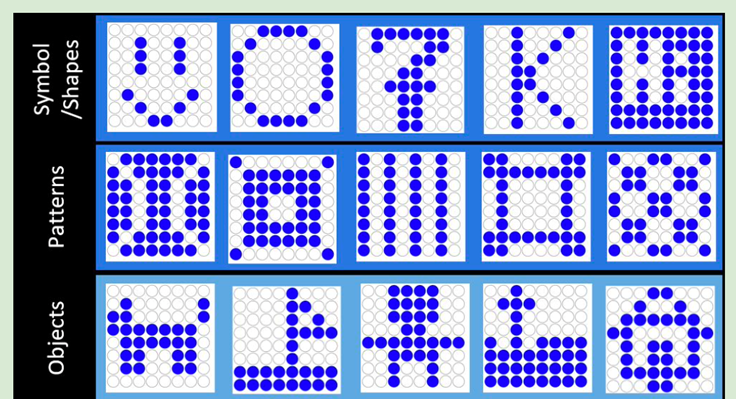
\includegraphics[width=0.7\textwidth]{images/diggs.png}
    \captionsetup{justification=centering}
    \caption[Some creations from the free-play study on humans by \cite{diggs}.]{Some creations from the free-play study on humans by \cite{diggs}.\\(Taken from the original publication.)}
    \label{fig:diggs}
\end{figure}
% \vspace{12pt}

% \todo{Find more references on this bias towards semantics in cognitive science}
% Cedric Collas and Pierre-Yves Oudeyer have some papers on this bias towards semantics in developmental psychology.

In the context of artificial intelligence, self-supervised learning has been a topic of interest for researchers in the fields of robotics and machine learning (ML), and the ability to efficiently and sufficiently explore remains a fundamental challenge.
In recent years, reinforcement learning (RL) has emerged as a powerful framework for training agents to learn complex behaviors through trial and error.
However, most RL algorithms are designed to solve specific tasks and are not well-suited for free-form exploration.
Instead, complementary formulations of novelty-based \cite{burda2018largescale,novel_explore} or uncertainty-based exploration \citep{rnd,plan_explore,disagreement} methods have been proposed to encourage agents to explore their environment in a self-supervised manner \citep{exploration_survey}. 
Yet, these methods are often unable to generate diverse and creative behaviors that are characteristic of human exploration.


% \todo{Play vs exploration}

% \todo{Comments on shaping of clip rewards near and far from the goal states}
% CLIP rewards are well-shaped around the goal state, whereas near the starting state, they are poorly shaped.

% \todo{Better segregate the different exploration methods (maybe in methods)}

% - Vision Language Models
This thesis focuses on the role of visual semantic bias in shaping these choices, proposing that our innate visual preferences act as a compass, directing our attention and interactions during free play.
Our work tries to imbue artificial agents with a visual semantics bias, akin to that in humans.
We do this by leveraging large vision language models (VLMs).
Also termed "foundational models", these deep neural networks are trained on massive generic text and image datasets using the recent advances in self-supervised learning. 
The abstractions of natural language, which reflect the semantics of the world, allow them to learn efficient representations that essentially encapsulate human visual understanding.

% - VLM Applications
VLMs are capable of successfully transferring to a diverse range of downstream applications, such as visual detection, classification, and question-answering.
However, the use of foundation models for control and embodied intelligence is relatively new and under-explored.

Pre-trained vision-language encoders, such as CLIP \citep{clip}, have been used far beyond their original scope such as image generation \citep{imagegeneration}, robot control \citep{cliport,embodied}

% In RL, pretraining has been used to improve the representations of the policy network. 
% Pretrained CLIP features have been used in various recent robotics papers to speed up control and navigation tasks.
% These features can condition the policy network [26] or can be fused throughout the visual encoder to integrate semantic information about the environment [37]. 
% The goal of these works is to improve the perception of the policy.
% Pretrained language models can also provide useful initializations for training policies to imitate offline trajectories [42, 27].
% These successes demonstrate that large pre-trained models contain prior knowledge that can be useful for RL. While the existing literature uses pre-trained embeddings directly in the agent, we instead allow the policy network to learn from scratch and only utilize pre-trained embeddings to guide exploration during training (Figure S2).
% We imagine that future work may benefit from combining both approaches.

% - VLM as Rewards
Recent work \citep{zest,negprompt,vlmrm,lamp} has shown that they can be used as effective abstractions to generate zero-shot rewards for language-guided goal-conditioned tasks.
There are also other studies on using VLMs for exploration \citep{vlmlang,vlmdistill} that use them for refining intrinsic reward signals by abstracting away pseudo-novelty. 

% - Entropy Rewards
Yet this is fundamentally different from our goal as we are specifically interested in creative semantic expression.
Moreover, the existing studies do not consider the free-form exploration paradigm that is of interest to us; they require a specific goal to be achieved, either self-generated or manually defined.
We instead use VLMs to generate exploratory intrinsic rewards that incentivize the agent to play with the environment and build something meaningful.
This reward is based on minimizing the entropy of a VLM's predictions over a set of creative possibilities that the environment offers.
Without any explicit goal specification, our controller exploits this reward to guide the agent to semantically expressive states, i.e. to automatically converge to an emergent state that the VLM finds confidently meaningful.

% - RaIR (Regularity as Intrinsic Reward)
Furthermore, since there is an implicit structure in meaningful creations, and given the compositional strategies for creative expression learned by humans during development \citep{symmetry,compositional} that favor symmetry and uniformity, we hypothesize that a complementary reward for this regularity \citep{rair} could promote semantic expression.

We test our formulations in two rich creative environments: the puzzle Tangram and a pixel grid, where we are able to achieve the desired semantically expressive behavior in our planning agent.
% We show the effect of all the different bells and whistles in an ablation study.

This thesis provides a novel perspective on imbuing free-form creativity in artificial agents and furthers the use of VLMs as a source of rewards in robotics and AI.

% The Methods section should be brief but adequate to allow a qualified investigator to repeat the research. The animals, supplies and equipment used should be described in detail. All companies from which compute resources were obtained should be listed with their location. All methods of analysis and statistical testing must be identified and explained in detail. Studies employing animals have to identify that the experiments being reported were approved by the Institutional Animal Care and Use Committee.
\chapter{Methods}
\label{sec:methods}

We use a family of VLMs called CLIP \citep{clip} for semantic inference and a model-based planning controller using an improved Cross-Entropy Method (iCEM) \citep{icem} as our artificial agent.
This chapter describes the components of our approach, including the mathematical setup, the CLIP model, the intrinsic semantics rewards, and the iCEM controller.

\section{Preliminaries}
\label{sec:preliminaries}
% - Notation
We formulate the problem as a \emph{fully observable} Markov Decision Process (MDP) given by the tuple \((\cS, \cA, \cO, \Theta, \Gamma, R, \bfs_0, \bfo_0)\), with state-space \(\cS \in \nR^{n_s}\), action-space \(\cA \in \nR^{n_a}\), observation-space (image-space) \(\cO \in \nR^{n_o}\), rendering function \(\Theta: \cS \mapsto \cO\), transition kernel (environment model) \(\Gamma: \cS \times \cA \mapsto \cS\), reward function \(R: \cS \times \cO \mapsto \nR\), initial state \(\bfs_0 \in \cS\), and its corresponding initial image observation \(\bfo_0 = \Theta(\bfs_0)\).

A trajectory \(\cT_t = \{(\bfs_t, \bfo_t, r_t, \bfa_t), (\bfs_{t+1}, \bfo_{t+1}, r_{t+1}, \bfa_{t+1}), \ldots \}\) at time \(t\) is a sequence of observation-reward-action tuples starting from the current state \(\bfs_t\), where \(\bfs_k \in \cS\), \(\bfo_k \in \cO\), \(r_k \in \nR\), and \(\bfa_k \in \cA\).
In a typical reinforcement learning (RL) setting, the returns of such a trajectory \(\cT_t\) are the discounted sum of rewards given by,
\begin{equation}
    \label{eq:rl-goal}
    \mathit{\Upsilon}(\cT_t) = \sum_{k=0} \gamma^k r_{t+k},
\end{equation}
where \(r_t\) is the expected reward at time \(t\) and \(\gamma \in [0, 1]\) is the discount factor. The agent's goal is to learn an action policy \(\pi^*: \cS \mapsto \cA\) that maximizes its expected reward;
\begin{equation}
    \label{eq:rl-policy}
    \pi^*_t = \argmax_{\pi} E_{\cT_t \sim \pi} \left[ \mathit{\Upsilon}(\cT_t) \right],
\end{equation}
where the expectation is under trajectories \emph{rolled-out} with \(\bfa_t \sim \pi(\cdot \mid \bfs_t)\), \(\bfs_{t+1} = \Gamma(\bfs_t, \bfa_t)\), \(\bfo_t = \Theta(\bfs_t)\), and \(r_t = R(\bfs_t, \bfo_t)\).

In our formulations, we consider a finite-horizon problem, where the agent is tasked with optimizing the expected return over a limited planning horizon \(\eta\).

\blfootnote{\textbf{Notation}:
We follow the following notation conventions throughout the text, unless explicitly noted otherwise.
Scalars are denoted using lowercase letters, e.g. \(x \in \nR\), and scalar hyperparameters are specially denoted with lowercase Greek letters, eg. \(\chi\).
Vectors are denoted with boldface letters, e.g. \(\bfx \in \nR^n\).
Sets of vectors are denoted italicized boldface letters with a length indicator, e.g. \(\bmx^{(n)} = \{ \bfx_1, \ldots, \bfx_n \}\). The length indicator is omitted for readability at times.
Calligraphic letters are used for higher vector sets, e.g. \(\cX = \{ \bmx^{(n)}_1, \ldots, \bmx^{(n)}_m \}\), and other sets, including spaces (\(\cS, \cA, \cO, \cI, \cL, \cV\)).
Functions are denoted by uppercase letters, e.g. \(\mathrm{X}\), and those with scalar codomains are italicized, eg. \(X\).
This is also true for the reward function denoted by \(R\) whose value is denoted by \(r\). This is not usually the case in RL literature (which denotes them just in the opposite way), but we use this notation to maintain consistency.
However, to avoid radically diverging from the prevalent notations, there are two notable exceptions -- \(\pi\) is used to denote the policy function and \(p\) for probability distributions.
% ``\(r\)'' for denoting reward functions. ``\(R\,\)'' instead denotes a scalar reward value.
}

\newpage    
\section{Vision-Language Models}
\label{sec:vlms}

We define vision-language models (VLMs) as functions capable of processing both language inputs \(\bml \in \cL\) and vision inputs \(\bmi \in \cI\), where \(\cL\) is a set of natural language strings/prompts and \(\cI \subseteq \cO\) is the space of 2D RGB images.

\subsection{CLIP}
\label{sec:clip}
CLIP (Contrastive Language Image Pretraining; \cite{clip}) is a family of vision-language models that have two main components -- an image encoder \(\Psi_I: \cI \mapsto \cV\) and a language encoder \(\Psi_L: \cL \mapsto \cV\), which generate unit magnitude vector embeddings for images and text, respectively, in the same high-dimensional latent space \(\cV \in [0, 1]^{n_v}\), which can thus be compared to each other using a vector similarity metric \(\Lambda: \cI \times \cL \mapsto \nR\), e.g. cosine similarity (\(S_c\), essentially dot product).

For a label \(\bfl \in \cL\) and an image \(\bfi \in \cI\), the similarity is given by,
\begin{equation}
    \label{eq:clip-similarity}
    \Lambda(\bfi, \bfl) := S_c(\Psi_I(\bfi), \Psi_L(\bfl)) = \dfrac{\Psi_I(\bfi) \cdot \Psi_L(\bfl)}{\| \Psi_I(\bfi) \| \| \Psi_L(\bfl) \|} = \Psi_I(\bfi) \cdot \Psi_L(\bfl).
\end{equation}

Eponymously, the CLIP image and text encoders are jointly trained using a contrastive loss which directs the model to semantically align the correct image and text pairs (in the latent space) by increasing their similarity while simultaneously pushing apart the embeddings of the mismatched pairs by decreasing their similarity.

Given a batch of \(n\) image-caption pairs; images \(\bmi^{(n)} = \{ \bfi_1, \dots, \bfi_{n} \}\) and captions \(\bml^{(n)} = \{ \bfl_1, \dots, \bfl_{n} \}\), such that the corresponding entries are paired, CLIP first computes the matrix of cosine similarities, \(\bmLambda^{(n)}(\bmi, \bml) \in \nR^{n \times n}\), where each item \(\bmLambda^{(n)}_{j,k}\) computes the cosine similarity between the image \(\bfi_j\) and caption \(\bfl_k\).
The training batch loss is then computed as the difference between the similarities corresponding to the correct image-caption pairs and the mismatched caption-image pairs, which is then minimized.

There are several variants of CLIP, with different sizes and different architectures for its image encoder (vision transformer \emph{ViT}; \cite{vit}, or residual network \emph{ResNet}; \cite{resnet}).
We used the vision transformer variant (\texttt{ViT-L/14}) for most of our experiments as it gave a good balance of performance and computational efficiency.
It takes image inputs of size \(224 \times 224\) and tokenizes them in patch sizes of \(14 \times 14\) for the vision transformer.
The comparison of the different models from the original paper for our use case is presented in Chapter \ref{sec:clip-comparison} of the appendix.

\subsubsection{CLIP as Zero-Shot Image Classifier}
\label{sec:clip-classifier}
CLIP can be used as a zero-shot classifier by comparing the embeddings of a given image and a set of prompts to predict the likelihood of the image belonging to each of the classes.

Given an image \(\bfi\) and a set of text prompts \(\bml\), the likelihood of the image belonging to the class described by a prompt \(\bfl_k \in \bml\) is given by the softmax function over the similarity scores of the image and the prompt embeddings,
\begin{equation}
    \label{eq:clip-dist}
    P(\bfl_k; \bfi, \bml, \tau) := \dfrac{\exp(\Lambda(\bfi, \bfl_k)/\tau)}{\sum_{\bfl_j \in \bml} \exp(\Lambda(\bfi, \bfl_j)/\tau)},
\end{equation}
where \(\tau \in \nR^+\) is the temperature hyperparameter that controls the flatness of the distribution.
This is an important parameter as it directly controls the quality of our entropy reward \eqref{eq:entropy-reward}.
The original paper suggests a value of \(0.01\) for most purposes, but we usually use values between the range \(0.01 - 0.02\) for our experiments.
See \secref{sec:reg-temperature} for details.

\subsubsection{Prompts for CLIP}
\label{sec:prompt-engineering}
Due to the inherent ambiguity in natural language, the exact phrasing can influence CLIP's inference.
We experiment with this in our investigations.

For objective analysis, we break the structure of a language prompt \(\bfc \in \cL\) representing a creative possibility \(c\) in an environment as ``\(\{\text{prefix}\}\{c\}\{\text{suffix}\}\)'', where ``prefix'' and ``suffix'' are optional context phrases. For example, if \(c =\) ``\texttt{apple}'', then the prompt could be ``\texttt{picture of an apple, on a white background}'', where ``\texttt{picture of an }'' and ``\texttt{, on a white background}'' are the prefix and suffix respectively.

\section{Semantic Rewards for Free Play}
\label{sec:semantics-reward}
This section describes the mathematical formulation of the intrinsic semantic reward that encourages the agent to explore its environment in a semantically expressive manner, akin to free play in humans.
It also gives the necessary background on the additional intrinsic regularity reward that complements it.

\subsection{Semantics Entropy Reward}
\label{sec:entropy-reward}
% - Entropy reward and its regularization hyperparameters derived from the ZEST formulation

Mathematically, in its simplest form, the semantics reward \(R_{\text{semantics-entropy}}: \cO \mapsto \nR\) is formulated as the negative entropy (\(-H\)) of the likelihood of the predictions of the VLM for an image observation \(\bfo \in \cO\) over a set of \(n_c\) creative possibilities \(\bmc = \{ \bfc_1, \bfc_2, \ldots, \bfc_{n_c} \}\);
We call this the \emph{semantics-entropy reward},
\begin{equation}
    \label{eq:entropy-reward}
    R_{\text{semantics-entropy}}(\bfo; \bmc, \tau) := -H(p(\bmc \mid \bfo; \tau)) = \sum_{\bfc_k \in \bmc} P(\bfc_k \mid \bfo; \bmc, \tau) \log P(\bfc_k \mid \bfo; \bmc, \tau).
\end{equation}
% 
\subsubsection{Goal-Baseline Regularization}
\label{sec:goal-baseline}
To improve the reward quality (shape), we further extend this formulation by adopting a combination of suggestions from other studies on VLMs as a source of goal-conditioned rewards.

The most trivial way to use CLIP as a goal-conditioned reward is to directly use the similarity metric from \eqref{eq:clip-similarity} as the reward function.
Given a goal description \(\bfg \in \cL\), the reward for an image observation \(\bfo \in \cO\) is given by,
\begin{equation}
    \label{eq:trivial-reward}
    R_{\text{clip}}(\bfo; \bfg) := S_c(\Psi_I(\bfo), \Psi_L(\bfg)).
\end{equation}
This captures the projection of the image observation embedding \(\bfo\) onto the direction spanned by the goal embedding \(\bfg\).

\cite{zest} developed an alternative method called \emph{ZeST} (zero-shot task specification) which employs \emph{delta embeddings} that use the difference in embeddings between the desired and initial/\emph{baseline} configurations, for both image and text inputs, to directionally remove irrelevant parts of the CLIP representation.
The goal-baseline regularized reward function in this case is the similarity between the delta embeddings,
\begin{equation}
    \label{eq:zest}
    R_{\text{zest}}(\bfo; \bfo_b, \bfg, \bfg_b) := S_c((\Psi_I(\bfo) - \Psi_I(\bfo_b)), (\Psi_L(\bfg) - \Psi_L(\bfg_b))).
\end{equation}
where \(\bfg_b \in \cL\) is a natural language description of the initial/baseline environment image observation \(\bfo_b = \bfo_0\).

Intuitively, providing a baseline sets the context of the setup, and the direction from a baseline \(\bfg_b\) to goal \(\bfg\) captures the desired change from the environment's image baseline \(\bfo_b\) to the target state.
As an example, consider the case where the goal is to draw a circle starting from a blank canvas i.e. the goal \(\bfg\) is something like ``a circle on a white background''.
Then the baseline \(\bfg_b\) could be ``a blank canvas'' and the image observation baseline \(\bfo_b\) would be the starting blank canvas image.

\cite{negprompt} further proposed a negative prompt formulation that used the negations of goal states, instead of descriptions of the initial states, as goal baselines.
In the example, this would be ``not a circle on a white background''.

These delta embeddings considerably improve performance in language-guided goal-conditioned tasks by providing a more focused reward signal.
However, it is not certain that the direction from the baseline to the goal captures all the relevant information.
Therefore, instead of using one or the other, \cite{vlmrm} further made a trade-off between the two projections in their \emph{VLM-RM} method and proposed a goal-baseline regularization technique that considered both -- the similarity of the image observation to the target and also the direction from the baseline towards the goal in the CLIP embedding space.

VLM-RM does not use delta embeddings or baselines for the image input, but only for the text input.
Their formulation is given by,
\begin{equation}
    \label{eq:vlmrm}
    R_{\text{goal-reg}}(\bfo; \bfg, \bfg_b, \gamma) := 1 - \dfrac{1}{2}\ \norm{\gamma\ \text{proj}_{\bfv}\Psi_I(\bfo) + (1 - \gamma)\ \Psi_I(\bfo) - \Psi_L(\bfg)}^2_2,
\end{equation}
where \[\bfv := \frac{\Psi_I(\bfg) - \Psi_L(\bfg_b)}{\norm{\Psi_I(\bfg) - \Psi_L(\bfg_b)}}\] is the direction spanned by the vector between the embeddings of \(\bfg\) and \(\bfg_b\), \[\text{proj}_{\bfv}\Psi_I(\bfo) := (\bfo \cdot \bfv)\,\bfv\] is the projection of the image observation embedding \(\bfo\) onto this direction, and \(\gamma \in [0, 1]\) is a hyperparameter to control the trade-off/regularization strength\footnote{We want to note here that the official implementation of VLM-RM available at \url{https://github.com/AlignmentResearch/vlmrm} is slightly different from the formulation given in the original paper, which is used here. Simplifying the other formulation leads to an additional term in the reduced form, but the overall essence of the reward from a conceptual standpoint still holds.}.
% 
% \begingroup
% \allowdisplaybreaks
\vspace{-1.5pt}
\begin{align}
    % R_{\text{goal-reg}}(\bfo; \bfg, \bfg_b, \gamma) &= 1 - \dfrac{1}{2}\ \norm{\gamma\ \text{proj}_{\bfv}\Psi_I(\bfo) + (1 - \gamma)\ \Psi_I(\bfo) - \Psi_L(\bfg)}^2_2, \label{eq:vlmrm}
    % \intertext{where \(\bfv\) is the direction spanned by \(\Psi_I(\bfg_b) - \Psi_L(\bfg)\), \(\text{proj}_{\bfv}\Psi_I(\bfo)\) is the projection of the image observation embedding \(\bfo\) onto this direction, and \(\gamma \in [0, 1]\) is a hyperparameter to control the regularization/trade-off strength.
    % Note that the magnitude of the projection \(\norm{\text{proj}_{\bfv}\Psi_I(\bfo)}_2\) is equivalent to the cosine similarity \(\cos(\vartheta) := S_c(\Psi_I(\bfo), (\Psi_L(\bfg) - \Psi_L(\bfg_b)))\), and \(\sin(\vartheta)\) is the projection of \(\bfo\) perpendicular to this direction.
    % The authors found this method to be relatively robust to changes in \(\gamma\) with most intermediate values being better than \(0\) or \(1\).}
    \shortintertext{For \(\gamma = 0\), the original CLIP similarity metric from \eqref{eq:clip-similarity} is recovered as an unregularized goal-conditioned reward function after simplification (since all embeddings are unit vectors, i.e. \(\norm{\Psi(\cdot)}_2 = 1\));}
    R_{\text{goal-reg}}(\bfo; \bfg, \bfg_b, 0) &= 1 - \dfrac{1}{2}\ \norm{\Psi_I(\bfo) - \Psi_L(\bfg)}^2_2 = S_c(\Psi_I(\bfo), \Psi_L(\bfg)). \label{eq:vlmrm-0}
    \intertext{For \(\gamma = 1\), there is a trade-off of components of \(\bfo\) orthogonal and parallel to ``\(\bfg - \bfg_b\)''.
    % Thus, it only retains the components that align with the direction from the baseline to the goal.
    % \texttt{-- A claim from the original paper; is incorrect!}
    }
    R_{\text{goal-reg}}(\bfo; \bfg, \bfg_b, 1) &= 1 - \dfrac{1}{2}\ \norm{\text{proj}_{\bfv}\Psi_I(\bfo) - \Psi_L(\bfg)}^2_2\\
    &= 1 - \dfrac{\norm{\text{proj}_{\bfv}\Psi_I(\bfo)}^2_2 + 1 - 2\ \text{proj}_{\bfv}\Psi_I(\bfo) \cdot \Psi_L(\bfg)}{2}\\
    &= \underbrace{\dfrac{1 - \norm{\text{proj}_{\bfv}\Psi_I(\bfo)}^2_2}{2}}_{\propto\ \sin^2(\vartheta)} + \underbrace{\dfrac{\Psi_I(\bfo) \cdot (\Psi_L(\bfg) - \Psi_L(\bfg_b))}{2}}_{\propto\ \cos(\vartheta)}. \label{eq:vlmrm-1}
\end{align}
% (Refer to equations \eqref{eq:vlmrm-equivalence-start} to \eqref{eq:vlmrm-equivalence-end} for more details on the derivation.)\\
% Mathematically, this is not equivalent to \eqref{eq:zest} (with no image baseline), because of the additional term, but it is similar in spirit.
% \endgroup

Note that the magnitude of the projection \(\norm{\text{proj}_{\bfv}\Psi_I(\bfo)}_2\) is equal to the cosine similarity \(\cos(\vartheta) := S_c(\Psi_I(\bfo), (\Psi_L(\bfg) - \Psi_L(\bfg_b)))\), and \(\sin(\vartheta)\) is the projection of \(\Psi_I(\bfo)\) perpendicular to this direction.

The authors found this method to be relatively robust to changes in \(\gamma\) with most intermediate values being better than \(0\) or \(1\).

\newpage
\subsection{Regularized Semantics Entropy Reward}
\label{sec:entropy-reward-reg}
We combine these ideas below to derive a \emph{baseline regularized semantics-entropy reward} from \eqref{eq:entropy-reward}.\\
Let \(\bmp := \text{proj}_{\bfv}\Psi_I(\bfo)\), \(\bmo := \Psi_I(\bfo),\ \bmg := \Psi_L(\bfg),\ \bmg_b := \Psi_L(\bfg_b)\) for brevity, then using the property \(\norm{\bmo}_2 = \norm{\bmg}_2 = \norm{\bmg_b}_2 = 1\) and the results \(\bmp \cdot \bmo = \norm{p}^2_2\) and \(\bmp \cdot \bmg = (\bmg - \bmg_b) \cdot \bmo\ /\ 2\), the VLM-RM reward can be simplified as,
\vspace{-1.5pt}
\begin{align}
    &1 - \dfrac{1}{2} \norm{\gamma\ \bmp + \left(1 - \gamma\right) \bmo - \bmg}^2_2 \tag{\(R_{\text{goal-reg}}\), from \ref{eq:vlmrm}}\\
    \label{eq:vlmrm-equivalence-start}
    &= 1 - \dfrac{1}{2} \Big[\norm{\gamma\ \bmp + \left(1 - \gamma\right) \bmo}^2_2 + \cancelto{1}{\norm{\bmg}^2_2} &&- 2 \left(\gamma\ \bmp + \left(1 - \gamma\right) \bmo\right) \cdot \bmg\Big]\\
    &= \dfrac{1 - \norm{\gamma\ \bmp + \left(1 - \gamma\right) \bmo}^2_2}{2} &&+ \gamma\ \bmp \cdot \bmg + \left(1 - \gamma\right) \bmo \cdot \bmg\\
    &= \dfrac{1 - \norm{\gamma \left(\bmp - \bmo\right) + \bmo}^2_2}{2} &&+ \dfrac{\gamma}{2} \left(\bmg - \bmg_b\right) \cdot \bmo + \left(1 - \gamma\right) \bmg \cdot \bmo\\
    &= \dfrac{1 - \gamma^2\ \norm{\bmp - \bmo}^2_2 - 2 \gamma \left(\bmp - \bmo\right) \cdot \bmo - \cancelto{1}{\norm{\bmo}^2_2}}{2} &&+ \left(\dfrac{\gamma}{2} \left(\bmg - \bmg_b\right) + \left(1 - \gamma\right) \bmg\right) \cdot \bmo\\
    &= \dfrac{-\gamma^2 \left(\norm{\bmp}^2_2 + \norm{\bmo}^2_2 - 2\ \bmp \cdot \bmo\right) - 2 \gamma \left(\bmp \cdot \bmo - \norm{\bmo}^2_2\right)}{2} &&+ \left(\dfrac{\gamma}{2}\ \bmg - \dfrac{\gamma}{2}\ \bmg_b + \bmg - \gamma\ \bmg\right) \cdot \bmo\\
    % &= \dfrac{-\gamma^2 \big(\norm{\bmp}^2_2 + \cancelto{1}{\norm{\bmo}^2_2} - 2\ \bmp \cdot \bmo\big) - 2 \gamma \big(\bmp \cdot \bmo - \cancelto{1}{\norm{\bmo}^2_2}\big)}{2} &&+ \left(\dfrac{\gamma}{2}\ \bmg - \dfrac{\gamma}{2}\ \bmg_b + \bmg - \gamma\ \bmg\right) \cdot \bmo\\ % above with cancellations
    &= \dfrac{-\gamma^2 \left(\norm{\bmp}^2_2 + 1 - 2\ \norm{\bmp}^2_2\right) - 2 \gamma \left(\norm{\bmp}^2_2 - 1\right)}{2} &&+ \left(\bmg - \dfrac{\gamma}{2}\ \bmg - \dfrac{\gamma}{2}\ \bmg_b\right) \cdot \bmo\\
    &= \dfrac{-\gamma^2 + 2\gamma}{2} + \dfrac{\gamma^2\ \norm{\bmp}^2_2 - 2 \gamma\ \norm{\bmp}^2_2}{2} &&+ \left(\left(1 - \dfrac{\gamma}{2}\right) \bmg - \dfrac{\gamma}{2}\ \bmg_b\right) \cdot \bmo\\ % additional step
    %% Option 1 -- p^2 term
    &= \gamma\left(1 - \dfrac{\gamma}{2}\right)\left(1 -\norm{\bmp}^2_2\right) &&+ \left(\left(1 - \dfrac{\gamma}{2}\right) \bmg - \dfrac{\gamma}{2}\ \bmg_b\right) \cdot \bmo\\
    &= \underbrace{\gamma\left(1 - \dfrac{\gamma}{2}\right)\left(\sin\left(\vartheta\right)\right)}_{\text{Term \#1 (\(\perp\))}} &&+ \underbrace{\left(\left(1 - \dfrac{\gamma}{2}\right) \bmg - \dfrac{\gamma}{2}\ \bmg_b\right) \cdot \bmo}_{\text{Term \#2 (\(\parallel\))}}.
    %% Option 2 -- constant term separated
    % &= \gamma\left(1 - \dfrac{\gamma}{2}\right) -\ \gamma \left(1 - \dfrac{\gamma}{2}\right)\norm{\bmp}^2_2 &&+ \left(\left(1 - \dfrac{\gamma}{2}\right) \bmg - \dfrac{\gamma}{2}\ \bmg_b\right) \cdot \bmo\\
    % &= \underbrace{\gamma\left(1 - \dfrac{\gamma}{2}\right)}_{\textstyle\text{constant}} -\ \underbrace{\gamma \left(1 - \dfrac{\gamma}{2}\right)\left(\bmo \cdot \dfrac{\left(\bmg - \bmg_b\right)}{\norm{\bmg - \bmg_b}_2}\right)^2}_{\text{Term \#1 (\(\perp\))}} &&+ \underbrace{\left(\left(1 - \dfrac{\gamma}{2}\right) \bmg - \dfrac{\gamma}{2}\ \bmg_b\right) \cdot \bmo}_{\text{Term \#2 (\(\parallel\))}}.
    \label{eq:vlmrm-equivalence-end}
\end{align}
Term \#1 captures the projection perpendicular to the direction from the baseline to the goal and Term \#2 captures the trade-off of projection along this direction and the goal.
To simplify further, we consider only the latter in our formulation as it contains the desired information about the goal.
We adopt this term as the basis to add baseline regularization to the semantics-entropy reward in \eqref{eq:entropy-reward-reg} and consider similar delta embeddings for the image observation space as well.

First, let us formulate a regularized similarity metric for an image observation \(\bfi \in \cI\) with baseline image \(\bfi_b \in \cI\) and target label \(\bfl \in \cL\) with baseline \(\bfl_b \in \cL\);
\begin{equation}
    \label{eq:clip-similarity-reg}
    \begin{split}
        \hat{\Lambda}(\bfi, \bfl; \bfi_b, \bfl_b, \alpha_{l}, \beta_{i})
        &:= S_c(
            ((1 - \beta_{i})\ \Psi_I(\bfi) - \beta_{i}\ \Psi_I(\bfi_b)),
            ((1 - \alpha_{l})\ \Psi_L(\bfl) - \alpha_{l}\ \Psi_L(\bfl_b))
        ),
    \end{split}
\end{equation}
where \(\alpha_{l}, \beta_{i} \in [0, 0.5]\) are the regularization hyperparameters homologous to \(\gamma / 2\) in \eqref{eq:vlmrm-equivalence-end}, for text and image inputs respectively, and \(\tau \in \nR^+\) is the temperature hyperparameter.

The updated likelihood distribution \(\hat{p}\) of the predictions of the VLM for the image observation \(\bfo \in \cO\) over the creative possibilities \(\bmc \subset \cC\) using this regularized similarity metric is then given by,
\begin{equation}
    \label{eq:clip-dist-reg}
    \hat{P}(\bfc_k \mid \bfo; \bfo_b, \bmc, \bfc_b, \alpha_{l}, \beta_{i}, \tau) := \dfrac{\exp(\hat{\Lambda}(\bfo, \bfc_k; \bfo_b, \bfc_b, \alpha_{l}, \beta_{i})/\tau)}{\sum_{\bfc_j \in \bmc} \exp(\hat{\Lambda}(\bfo, \bfc_k; \bfo_b, \bfc_b, \alpha_{l}, \beta_{i})/\tau)},
\end{equation}
where \(\bfc_k \in \bmc\). Using these definitions, the regularized semantics-entropy reward is given as,
\begin{align}
    R_{\text{sem-entropy-reg}}(\bfo; \bfo_b, \bmc, \bfc_b, \alpha_{l}, \beta_{i}, \tau)
    &:= -H(\hat{p}(\bmc \mid \bfo; \bfo_b, \bfc_b, \alpha_{l}, \beta_{i}, \tau)) \label{eq:entropy-reward-reg}\\
    &\ = \sum_{\bfc_k \in \bmc} \hat{P}(\bfc_k \mid \bfo; \bfo_b, \bmc, \bfc_b, \alpha_{l}, \beta_{i}, \tau) \log \hat{P}(\bfc_k \mid \bfo; \bfo_b, \bmc, \bfc_b, \alpha_{l}, \beta_{i}, \tau), \nonumber
\end{align}
where \(\bfc_b\) is the text baseline, which could either be the initial state description or the negation of the goal.

\newpage
\subsection{Regularity Reward}
\label{sec:regularity-reward}
We complement the semantic reward with regularity as an intrinsic reward (\emph{RaIR}) \citep{rair}, which encourages the agent to create regular and symmetric patterns in its creations.
The authors described the regularity reward RaIR as ``(the) redundancy in the description of the situation, to measure the degree of sub-structure recurrence''.

Mathematically, we consider that the state space can be factorized into a composition of the different (\(n_e\)) entities in the environment and the configuration of the agent, \(\cS = (\cS_{\text{obj}})^{n_e} \times \cS_{\text{agent}}\), where \(\cS_{\text{obj}} \in \nR^d\); \(d = 2\) in our environments. %, such that \(n_s = n_e \cdot d\).
This allows the RaIR reward \(R_{\text{RaIR}}: \cS \mapsto \nR\) to be formulated in terms of multiplicities \(M: \cX \mapsto \nN\) (counts of occurrence) of the sub-structures \(\cX\) in the arrangement of the different entities of the environment in the state \(\bfs\),
\begin{equation}
    \label{eq:rair}
    R_{\text{RaIR}}(\bfs; \omega) := -H(\mathrm{\Omega}(\bfs; \omega)) = \sum_{\cX \in \mathrm{\Omega}(\bfs)} P(\cX; \omega) \log P(\cX; \omega),
\end{equation}
where \(\mathrm{\Omega}\) is a factorization function that decomposes a state \(\bfs\) into a multiset of its unique sub-structures given the hyperparameters \(\omega\) (resolution, bidirectionality),
\begin{equation}
    \label{eq:rair-factorization}
    \mathrm{\Omega} : (\cS_{obj})^{n_e} \mapsto \{ \cX_1^{M(\cX_1)}, \cX_2^{M(\cX_2)}, \ldots \},
\end{equation}
and \(P(\cX; \omega)\) is the probability of a sub-structure \(\cX \in \mathrm{\Omega}(\bfs; \omega)\) in the state \(\bfs\) calculated as,
\begin{equation}
    \label{eq:rair-probability}
    P(\cX; \omega) = \dfrac{M(\cX)}{\sum_{\cX' \in \mathrm{\Omega}(\bfs; \omega)} M(\cX')}.
\end{equation}
% 
For our purposes, following insights from \cite{symmetry} and \cite{compositional}, we use the relational formulation of RaIR which captures the pairwise relationships between the entities of the environment in the state \(\bfs\) by calculating the distances between them in the discretized coordinate space;
\begin{equation}
    \label{eq:rair-relational}
    \mathrm{\Omega}(\bfs) = \{ \cX^{M(\cX)} : \cX = \lfloor s^{(j)} - s^{(k)} \rceil \mid s^{(j)}, s^{(k)} \in \bfs \},
\end{equation}
where the \(\lfloor \cdot \rceil\) operator groups the distances into discrete bins based on the configured resolution.
For more details on the parameters and formulation, please refer to \secref{sec:regularity-reward-details} of the appendix.

\subsection{Complete Intrinsic Semantics Reward}
\label{sec:complete-semantics-reward}
The complete intrinsic semantics reward \(R_{\text{semantics}}\) is then given as the weighted sum of the regularity reward \(R_{\text{RaIR}}\) and the regularized semantics-entropy reward \(R_{\text{semantics-entropy-reg}}\);
\begin{equation}
    \label{eq:semantics-reward}
    R_{\text{semantics}}(\bfs, \bfo; \bfo_b, \bmc, \bfc_b, \alpha_{l}, \beta_{i}, \tau) =R_{\text{semantics-entropy-reg}}(\bfo; \bfo_b, \bmc, \bfc_b, \alpha_{l}, \beta_{i}, \tau) + \lambda\ R_{\text{RaIR}}(\bfs),
\end{equation}
where \(\lambda\) is a hyperparameter that controls the trade-off between the two rewards.

To be able to properly compare the two rewards, we constrain them to the same range \([0, 1]\) by normalizing them with their maximum possible entropy.
The regularity reward is normalized by the maximum possible entropy of the multiset -- \(\log\left(\binom{n_e}{2}\right)\), which is equal to the entropy of a uniform distribution over the \(\binom{n_e}{2}\) possible pairwise object distances of the \(n_e\) entities/objects in the state space, and
the semantics-entropy reward is normalized by the maximum possible entropy of the likelihood distribution over the creative possibilities, which is \(\log(n_c)\), where \(n_c\) is the number of creative possibilities.

\newpage
\section{iCEM}
\label{sec:icem}
% The Cross-Entropy Method (CEM) is an adaptive importance sampling procedure.

In the Model-Based Reinforcement Learning (MBRL) paradigm, the agent learns a model \(\Gamma\) of the MDP dynamics from interactions with the environment and uses it to predict the consequences of its actions which enables it to plan for the best policies.
Such policies can be learned with universal function approximators such as neural networks using RL algorithms or planning methods.

The improved Cross-Entropy Method (iCEM) is one such planning method.
It is a zeroth-order Monte-Carlo trajectory optimizer that works in a Model Predictive Control (MPC) loop to solve finite-horizon planning problems online, i.e. it iteratively re-plans after every step in the environment by (1) coming up with several action sequences (by sampling a multi-variate distribution) to \emph{think} a few steps ahead, (2) imagining/predicting the future states resulting from these actions (using the model of the environment) and assessing their expected returns (using the reward function), (3) picking out the best action sequences, (4) improving the \emph{thinking} method based on these elite sequences, and (5) taking the first step of the best action sequence.

Precisely, given a finite planning horizon \(\eta\), iCEM uses a clipped colored-noise Gaussian distribution of dimension \(n_a \times \eta\) over action sequences (\(\bma^{(\eta)} = \{ \bfa_0, \bfa_1, \ldots, \bfa_{\eta-1} \}\)), given by,
\begin{equation}
    \label{eq:icem-distribution}
    p(\bma^{(\eta)}) = \text{clip}(\bmmu_t + \cC^\beta(n_a, \eta) \odot \bmsigma_t^2),
\end{equation}
where \(\bmmu_{t}, \bmsigma_{t} \in \nR^{n_a \times \eta}\) are the mean and standard deviation of the sampling distribution at time \(t\) respectively, and \(\cC^\beta(n_a, \eta)\) is a sampling function that returns \(n_a\) (one for each action dimension) sequences of length \(\eta\) sampled from colored noise normal distribution with exponent \(\beta\) (\(= 1\) in our experiments; pink noise), zero mean, and unit variance.

At every timestep \(t\), there are multiple \emph{inner} iterations of the following calculations.
At inner iteration \(i\),\\
(1) starting with a sampling distribution \( p(\bmmu_{t}^{i - 1},\bmsigma_{t}^{i - 1})\), a fixed-length (\(\nu\)) set of action sequences (\(\cA_t = \{ \bma^{(\eta)}_1, \bma^{(\eta)}_2, \ldots, \bma^{(\eta)}_{\nu} \}\)) is sampled from this distribution.
These samples are augmented with a fraction \(\zeta\) of the best action sequences (called the \emph{elite-set} \(\cE_t^{i - 1}\)) from the previous inner iteration (called \emph{keep-elites}) or the previous timestep (called \emph{shift-elites}) if \(i = 0\); this is denoted by \(\zeta \cdot \cE_t^{i - 1}\) in \eqref{eq:icem-augment}. 
Additionally, to ensure that the mean action of the distribution is accessible to the controller, in the last inner iteration \(\iota\), the mean of the distribution \(\bmmu_t\) is added to the elite-set \(\cA^+\);
\begin{equation}
    \label{eq:icem-augment}
    \cA^+_t = \cA_t \cup \begin{cases}
            \zeta \cdot \cE_{t - 1}^\iota & \text{if } i = 0,\\
            \zeta \cdot \cE_t^{\iota - 1} \cup \{ \bmmu_t^\iota \} & \text{if } i = \iota,\\
            \zeta \cdot \cE_t^{i - 1} & \text{otherwise}.
    \end{cases}
\end{equation}

(2) Every action sequence in this augmented set \(\cA^+_t\) is then rolled out (\emph{in imagination}) using the environment model \(\Gamma\) and rendering function \(\Theta\) from the current state \(\bfs_t\) to predict their corresponding expected states and image observations respectively,
\vspace{-1.5pt}
\begin{align}
    \cS_t &= \{ \{ \bfs_{t+1}, \bfs_{t+2}, \ldots, \bfs_{t+\eta} \} \}_{j=1}^{\nu}, \label{eq:icem-rollout}\\
    \cO_t &= \{ \{ \bfo_{t+1}, \bfo_{t+2}, \ldots, \bfo_{t+\eta} \} \}_{j=1}^{\nu}, \label{eq:icem-observations}
    \intertext{where \(\bfs_t = \Gamma(\bfs_{t-1}, \bfa_{t-1})\) and \(\bfo_t = \Theta(\bfs_t)\). The predicted states are evaluated according to the reward function \(r\) to get their corresponding rewards,}
    \cR_t &= \{ \{ r_{t+1}, r_{t+2}, \ldots, r_{t+\eta} \} \}_{j=1}^{\nu}, \label{eq:icem-rewards}
\end{align}
where \(r_{t} = R(\bfs_t, \bfo_t) = \sum_k \lambda_k r_k(\bfs_t, \bfo_t)\) is the weighted sum of all the intrinsic rewards.
The corresponding trajectories are,
\begin{equation}
    \label{eq:icem-trajectories}
    \cT^{(\nu \times \eta)}_t = \{\{(\bfs_t, \bfo_t, r_t, \bfa_t), \ldots, (\bfs_{t+\eta-1}, \bfo_{t+\eta-1}, r_{t+\eta-1}, \bfa_{t+\eta-1}), (\bfs_{t+\eta}, \bfo_{t+\eta}, r_{t+\eta}, \varnothing) \}\}_{j=1}^{\nu}.
\end{equation}
% 
(3) Subsequently, a new elite-set of actions \(\cE_t^i\) of given size \(\kappa\) is determined; it consists of the best \(\kappa\) action sequence samples that maximize an aggregation of the returns from their expected states according to a reward aggregation function \(\mathit{\Upsilon}\);
\begin{equation}
    \label{eq:icem-filter}
    \cE_t^i = \kappa \cdot \cA^+_t = \underset{\text{Best \(\kappa\) action sequences in the augmented set of samples \(\cA^+_t\)}}{\{ \bma^{(\eta)}_k \in \cA^+_t :\ \mid \bma^{(\eta)}_j \in \cA^+_t : \mathit{\Upsilon}(\cT^{(\eta)}_k) \leq \mathit{\Upsilon}(\cT^{(\eta)}_j) \mid\ \leq \kappa \}}.
\end{equation}
More information about the reward aggregation strategies used in our experiments is provided in \autoref{sec:reward-aggregation}.

(4) These new elite action sequences are finally used to refine the distribution to maximize the expected return of its samples.
\vspace{-1.5pt}
\begin{align}
    \label{eq:icem-update}
    \bmmu_{t}^i &= \alpha\ \bmmu_t^{i - 1} + (1-\alpha)\bmmu^{\cE_t^i},\\
    (\bmsigma_{t}^i)^2 &= \alpha(\bmsigma_t^{i - 1})^2 + (1-\alpha)(\bmsigma^{\cE_t^i})^2,
\end{align}
where \(\alpha \in [0, 1]\) is a \emph{momentum} factor.

The above steps are repeated for \(\iota\) inner iterations at every timestep.
At the end of this process, the distribution concentrates on action sequences with high returns, and the best action sequence converges to an optimum;
\begin{equation}
    \label{eq:planning-goal}
    \bma^{(\eta)*} = \argmax_{\bma^{(\eta)}_k \in \cA^+} \mathit{\Upsilon}(\cT^{(\eta)}_k).
\end{equation}
(5) Finally, the first action of the best elite sequence of actions \(\bma^{(\eta)*}_t\) is executed in the environment.
The process is repeated for a specified number of rollout steps or until a terminal state or reward threshold is reached.

% There are additional features that the original iCEM implementation provides, such as decaying population size over time. 
Since the standard deviation in iCEM adapts according to the elite-set statistics, when the controller is close to an optimum, the standard deviation automatically decreases, narrowing down the search and fine-tuning the solution.
Therefore it is sufficient to sample fewer action sequences as the CEM iterations proceed.
Thus, the population size is exponentially decayed over time with factor \(\delta\). 
At timestep \(t\), it is equal to \(max(\nu \delta^{-t}, 2\kappa)\), where the max ensures that the population size is at least double the size of the elite-set.

Since iCEM is a zero-order trajectory optimizer with a limited sample budget and finite-horizon planning, we do not necessarily converge to the global optima.
Although this does not solve the full reinforcement learning problem (infinite horizon and stochastic environments), it is very powerful in optimizing for tasks ad-lib without further adaptation, which makes it suitable for optimizing changing exploration targets in sparse reward scenarios, as in our case (because of noisy CLIP rewards; discussed later in \secref{sec:inference-noise}).

The colored noise of the iCEM distribution leads to temporally correlated action sequences over the horizon for smoother trajectories, which helps mitigate the problems due to the noisy nature of our semantics entropy reward by effectively regularizing the reward landscape.
Furthermore, the addition of memory gives it good sample efficiency, which is essential for our case due to the computational bottleneck because of the long inference times for CLIP.
These reasons made iCEM a suitable choice for our experiments.

For this to be successful, a good transition model \(\Gamma\) needs to be learned, and the reward function needs to be known or discovered.
In our case, the reward function is well-defined, and to evaluate the efficacy of our entropy minimization objective in achieving good semantic expression,
we run simulations using ground truth (GT) models, i.e. with access to the true simulator of the environment itself.
Thus, we can perform multi-horizon planning without accumulating any model errors, which allows us to better investigate the shape and global/local optima of our semantics reward landscape. 

\subsection{Reward Aggregation Strategies}
\label{sec:reward-aggregation}
There are many different ways to aggregate the rewards of the trajectory samples over the horizon.
This is treated as one of the hyperparameters in our experiments.
\vspace{-13.5pt}
\begin{align}
\intertext{A trivial reward aggregation function is the sum of the rewards over the horizon (\texttt{sum}),}
\texttt{sum}(\cT^{(\eta)}) &= \sum_{k=1}^{\eta} r_k. \label{eq:reward-aggregation-sum}
\intertext{We further experimented with a discount factor \(\gamma \in \nR^+\) over the horizon, but usually set it to \(1.0\);}
\texttt{sum-\emph{\(\gamma\)}}(\cT^{(\eta)}) &= \sum_{k=1}^{\eta} \gamma^{k-1} r_k. \label{eq:reward-aggregation-sum-discount}
\intertext{However, this type of consolidating aggregation strategy is not suitable for cases where an increase in return can be preceded by an initial decrease (as a consequence of leaving local optima). So we also considered the \texttt{best} method, which uses the best return over the planning horizon;}
\texttt{best}(\cT^{(\eta)}) &= \max_{k=1}^{\eta} r_k. \label{eq:reward-aggregation-best}
\intertext{Additionally, to combine the better qualities of both the \texttt{sum} and \texttt{best} methods; we formulated a dynamic reward aggregation method that ranks trajectories based on the highest sum of consecutive rewards in a window of a predefined hyperparamterized length \(l\), \texttt{best-\emph{l}};}
\texttt{best-\emph{l}}(\cT^{(\eta)}) &= \max_{k=1}^{\eta-l+1} \sum_{j=k}^{k+l-1} r_{k+j}. \label{eq:reward-aggregation-best-dynamic}
\intertext{Another strategy is to assess the trajectories based on their last states (\texttt{last}), i.e. to simply consider only what the agent could potentially achieve at the end of the horizon.
This is particularly useful when inferring the reward is expensive, as in our case, because only one final state needs to be evaluated;}
\texttt{last}(\cT^{(\eta)}) &= r_h. \label{eq:reward-aggregation-last}
\intertext{Finally, we also experimented with a combination of the \texttt{sum} and \texttt{last} methods with \texttt{last-\emph{l}}, which is the sum of the returns of the last \(l\) steps of the trajectory;}
\texttt{last-\emph{l}}(\cT^{(\eta)}) &= \sum_{k=\eta-l+1}^{\eta} r_k. \label{eq:reward-aggregation-sum-last}
\end{align}

Note that we often use the term \emph{cost} (\(-1 \times r\)) instead of reward in our results and discussions. This is because the iCEM controller implementation we use minimizes costs instead of maximizing rewards, which are essentially equivalent, and only differ in their signs.

\section{Experiment Setup}
\label{sec:experiment-setup}

The simulations are run concurrently on multiple NVIDIA V100 and A100 GPUs, depending on the size of the simulations, which is determined by the size of the CLIP model used, the number of trajectory samples in iCEM, and the number of planning horizons.
To minimize the time of a rollout, all \(\eta \times \nu\) CLIP inferences for planning at an inner iCEM iteration are performed in a single batch in parallel.
Environment rendering and simulations are multi-processed on CPU in parallel.

Several optimizations were put into place to improve the simulation time, particularly in environment rendering and CLIP preprocessing.
Please refer to Chapter \ref{sec:efficiency} of the appendix for more details.

\section{Environments}
\label{sec:environments}
We use two custom environments in our experiments which allow for rich creative expression.

\begin{figure}[H]
    \centering
    \subfloat[\centering ShapeGridWorld]{\fbox{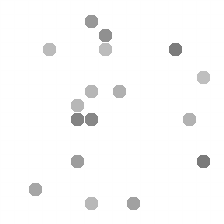
\includegraphics[width=0.4\textwidth]{images/sgw_random.png}}}
    \qquad
    \subfloat[\centering Tangram]{\fbox{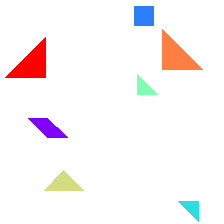
\includegraphics[width=0.4\textwidth]{images/tangram_random.png}}}
    \caption{The environments.}
    \label{fig:environments}
\end{figure}

\subsection{ShapeGridWorld}
\label{sec:sgw}
ShapeGridWorld (SGW) is a pixel grid environment where the agent can draw on the grid by moving pixels around, either one or all of them at the same time.
This is reminiscent of the pin-board platform used in the free play study conducted by \citet{diggs} (\figref{fig:diggs}).
By setting the pixels in a specific layout, the agent can draw a variety of shapes on the grid.
This environment is adapted from the pixel grid environment used in the work by \citet{rair} with some modifications summarised in \ref{sec:sgw-details} of the appendix.

ShapeGridWorld was mostly used in the initial experiments but it eventually proved to promote noise in CLIP inferences which led to underwhelming results.
To work around the problems, the Tangram environment was developed.

\subsection{Tangram}
\label{sec:tangram}
Tangram is a traditional puzzle game consisting of a canvas and seven geometric shapes -- five right isosceles triangles (two large, one medium, and two small), one square, and one parallelogram, which conventionally have distinct colors.
These shapes can be rotated, flipped, and translated on the canvas, without overlapping.
Even though this is a very simple setup, these pieces can be arranged in very different configurations to create expressive abstract patterns.

The Tangram virtual environment was developed specifically for our experiments.
Because of its reduced degrees of freedom compared to ShapeGridWorld, it mitigates the problems discussed in sections \secref{sec:noisy-rewards} and \secref{sec:inference-noise}.
It is a major contribution of our work.

We mostly configured the environment to correspond with the traditional Tangram game.
The shapes involved are the same, no overlap is allowed, and the shapes could be rotated, flipped, and translated.
Yet, we conducted experiments with colors to improve the performance of CLIP and also tested giving the agent the freedom to use a subset of the shapes to make its creations.

Please refer to \secref{sec:tangram-details} of the appendix for more technical details about this environment.

% The Experiments of the study should be laid out in a series of declarative paragraphs. Only results essential to establish the main points of the work should be included. Often the reporting of the results can be clearer if broken down into subsections. All figures and tables must be cited in the text and must be numbered in the order of their text citation. Figure legends should be self-explanatory, without referring to the text. They should identify the material that is being illustrated, what is shown, and its significance. Each table should be identified by number and should have a title. This section should not include long passages about the rationale of the experiments (which belong in the Introduction), or the methods used (which belong in the Material and Methods), nor should it include justification or discussion of the results (which belong in the Discussion section).
\chapter{Experiments}
\label{sec:experiments}

We perform these experiments to showcase that we can indeed get semantically expressive creations with our proposed formulation.

\section{Environments}
\label{sec:environments}
We use two custom environments in our experiments which allow for rich creative expression.

\begin{figure}[H]
    \centering
    \subfloat[\centering ShapeGridWorld]{\fbox{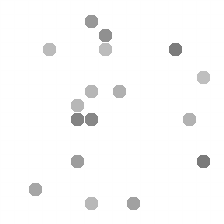
\includegraphics[width=0.4\textwidth]{images/sgw_random.png}}}
    \qquad
    \subfloat[\centering Tangram]{\fbox{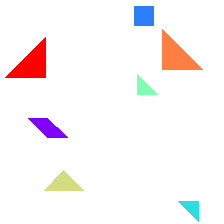
\includegraphics[width=0.4\textwidth]{images/tangram_random.png}}}
    \caption{The environments.}
    \label{fig:environments}
\end{figure}

\subsection{ShapeGridWorld}
\label{sec:sgw}
ShapeGridWorld is a pixel grid environment where the agent can draw on the grid by moving pixels around, either one or all of them at the same time.
This is reminiscent of the pin-board platform used in the free play study conducted by \citet{diggs} (\figref{fig:diggs}).
By setting the pixels in a specific layout, the agent can draw a variety of shapes on the grid.
This environment was adapted from the pixel grid environment used in the work by \citet{rair} with some modifications summarised in appendix \ref{sec:sgw-details}.

ShapeGridWorld was mostly used in the initial experiments but it later proved to promote noise in CLIP inferences which led to underwhelming results.
To work around the problems, the Tangram environment was developed.

\subsection{Tangram}
\label{sec:tangram}
Tangram is a traditional puzzle game consisting of a canvas and seven geometric shapes -- five right isosceles triangles (two large, one medium, and two small), one square, and one parallelogram, which conventionally have distinct colors.
These shapes can be rotated, flipped, and translated on the canvas, without overlapping.
Even though this is a very simple setup, these pieces can be arranged in very different configurations to create expressive abstract patterns.

The Tangram virtual environment was developed specifically for our experiments as it mitigated the problems discussed in sections \secref{sec:sparse-rewards} and \secref{sec:inference-noise}, and is a major contribution of our work.

We mostly configured the environment to correspond with the traditional Tangram game.
The shapes involved were the same, no overlap was allowed, and the shapes could be rotated, flipped, and translated.
Yet, we did experiments with colors to improve the performance of CLIP and also gave the agent the freedom to use a subset of the shapes to make its creations.
Please refer to appendix \ref{sec:tangram-details} for more technical details about this environment.

\section{Initial Tests with CLIP}
\label{sec:clip-custom}

% Talk about the initial tests with CLIP that were motivated by the poor performance of CLIP on abstract images and sketches.
CLIP was trained on a large dataset of captioned natural images foraged from the internet.
While it generalizes well to many natural-image distributions and has proved to be a powerful zero-shot model for various tasks, it was not clear how well it would perform on sketches and abstract images. 

CLIP has been shown to not perform much better than chance on some tasks as they were not well represented in its pre-training dataset.
% For example, it only achieved 88\% accuracy on the handwritten digits of MNIST.
The authors of CLIP also noted that it is particularly poor on tasks for fine-grained classification such as differentiating models of cars, species of flowers, and variants of aircraft.
It also struggles with more abstract and systematic tasks such as counting the number of objects in an image.

Moreover, \cite{vlmrm}, from their experiments with CLIP as a source of goal-conditioned rewards, reported that CLIP rewards are only meaningful and well-shaped for environments that are photorealistic enough for the CLIP visual encoder to interpret correctly.
They found that it is crucial to add textures and shading to the images to make them more realistic for CLIP to perform well.

Influenced by these observations and caveats, we suspected that our environments, since they are not photorealistic, might also be out-of-distribution. 
Yet, we expected them to be simple enough for CLIP to interpret correctly.

Thus, before testing our reward function, we conducted a series of simple experiments on the inference capabilities of CLIP on ShapeGridWorld and Tangram.
At the same time, there were several hyperparameters in the environments and CLIP into which we took insights with these initial tests.


\subsection{CLIP on Sketches and ShapeGridWorld}
\label{sec:clip-sketches}

We first tested CLIP on sketches of simple shapes from the ImageNet-Sketch dataset \citep{imagenet}.

We also compared these results with renderings of these sketches on ShapeGridWorld grids of different resolutions by registering them (see \secref{sec:sgw-registration} for more details).

\begin{figure}[H]
    \centering
    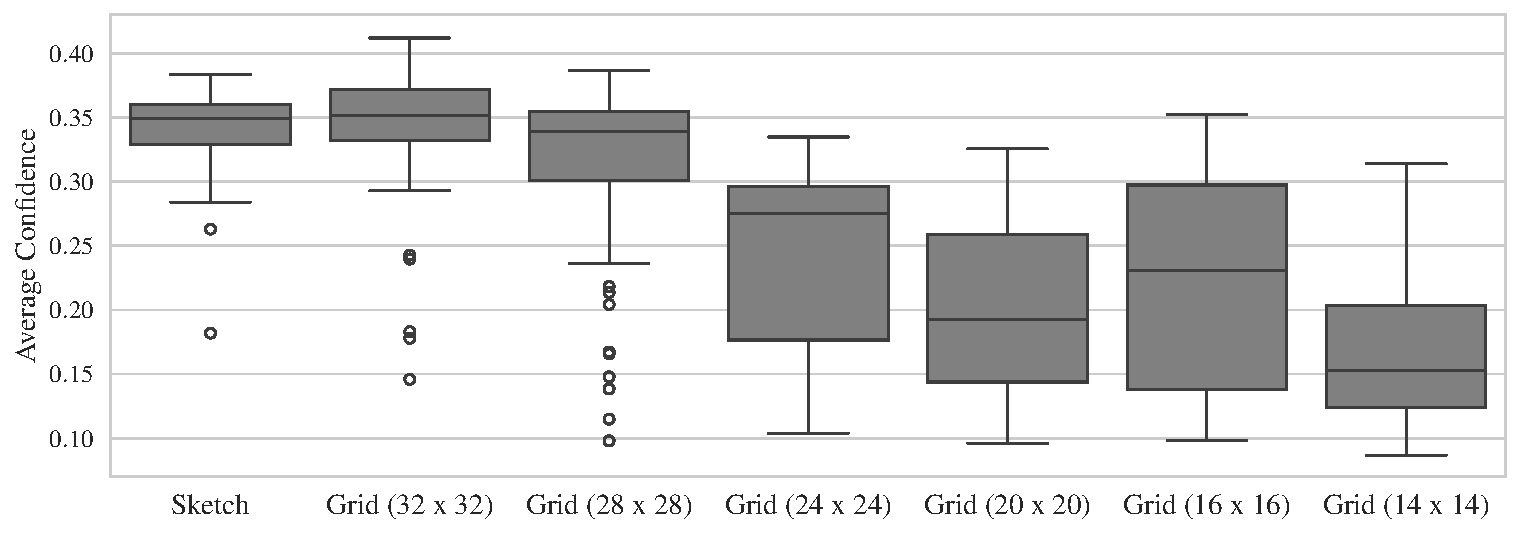
\includegraphics[width=\textwidth]{images/grid_comparison.pdf}
    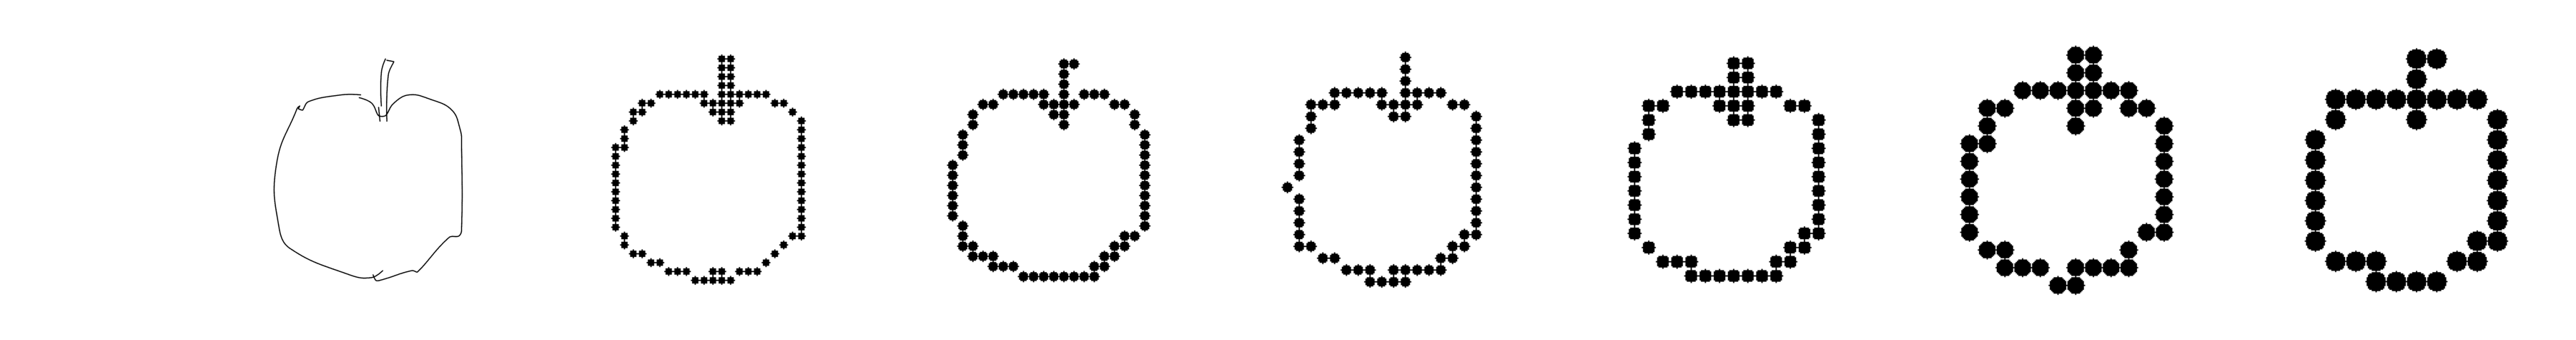
\includegraphics[width=\textwidth]{images/grid_comparison_images.png}
    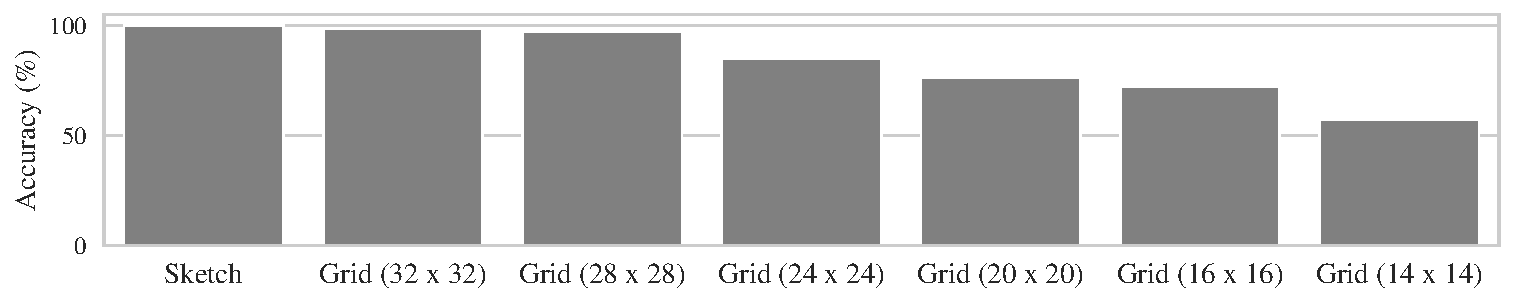
\includegraphics[width=\textwidth]{images/grid_comparison_accuracy.pdf}
    \caption{CLIP on sketches and ShapeGridWorld grids of different resolutions.}
    \label{fig:clip-sketches}
    % 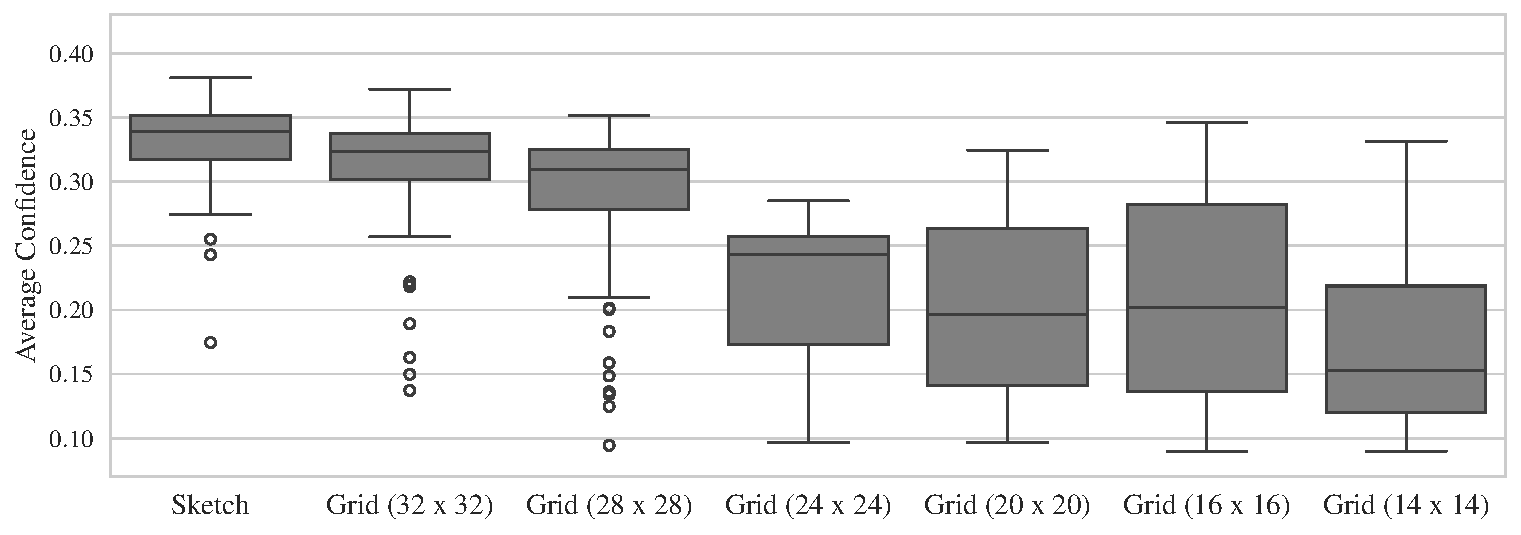
\includegraphics[width=\textwidth]{images/grid_comparison_inverted.pdf}
    % 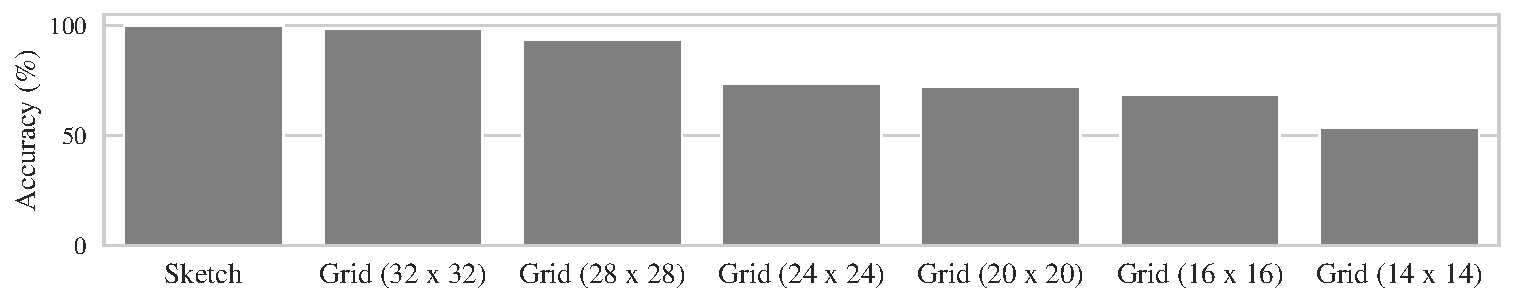
\includegraphics[width=\textwidth]{images/grid_comparison_accuracy_inverted.pdf}
    % \caption{CLIP on \emph{inverted} sketches and ShapeGridWorld grids of different resolutions.}
    % \label{fig:clip-sketches-inv}
\end{figure}

As an example, \figref{fig:clip-sketches} shows the comparative similarity of the embeddings of \(80\) sketches of apples (and their grid counterparts) to the label ``sketch of an apple'' using the CLIP variant \texttt{ViT-L/14}, as a probability.
The probabilities are calculated using the equation \eqref{eq:clip-dist}, with temperature \(T = 1\), to show the trend.
The categories for this example are ``apple'', ``chair'', ``car'', ``flower'', ``pencil'', ``house'', ``tree'', ``fish'', ``star'', and ``bird''.
The middle row shows a sample of the images for each of the cases.
The bottom row shows the accuracy (percentage of correct predictions) for each of the cases.

\begin{wrapfigure}{r}{0.4\textwidth}
    \centering
    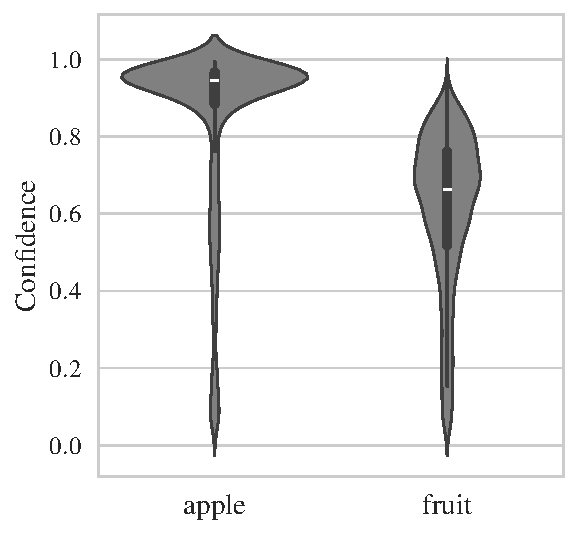
\includegraphics[width=0.36\textwidth]{images/hypercategory_comparison_2.pdf}
    \caption{CLIP on different specificity of labels.}
    \label{fig:clip-hypercategory}
\end{wrapfigure}

We found that CLIP can recognize these sketches quite well.
As the grid became coarser, the confidence and accuracy of CLIP decreased significantly.
For very coarse grids, the accuracy is almost as bad as random guessing.
We also experimented with inverting the images and found that results were consistently slightly better with black-on-white sketches (shown here) than with white-on-black sketches.
Yet, we did not notice any difference in performance with the addition of grayscale values in the pixel blocks.
In most cases, we also noticed that using specific labels like ``apple'' for a picture of an apple had better accuracy than using hypernyms like ``fruit'' (\figref{fig:clip-hypercategory}).

Additionally, we found that the bigger CLIP models performed significantly better on these tasks than the smaller ones which is in line with observations from other studies on VLMs as a source of rewards.
Furthermore, we tried the same experiments with different sets of categories, prefixes, and suffixes, but the results followed similar trends.
The later sections give more results for experiments on these hyperparameters.


\subsection{CLIP on Tangram}
\label{sec:clip-tangram}

Tangram has lesser degrees of freedom than ShapeGridWorld and it is more abstract but it still allows for rich creative expression.
To test if it would be a feasible environment for our study, we used some images of creations on Tangram from the internet and used CLIP as a zero-shot classifier as above to test its performance.
We again found it to be quite good at recognizing these creations with very high confidence.
\figref{fig:clip-tangram} shows a few examples.
\begin{figure}[h]
    \centering
    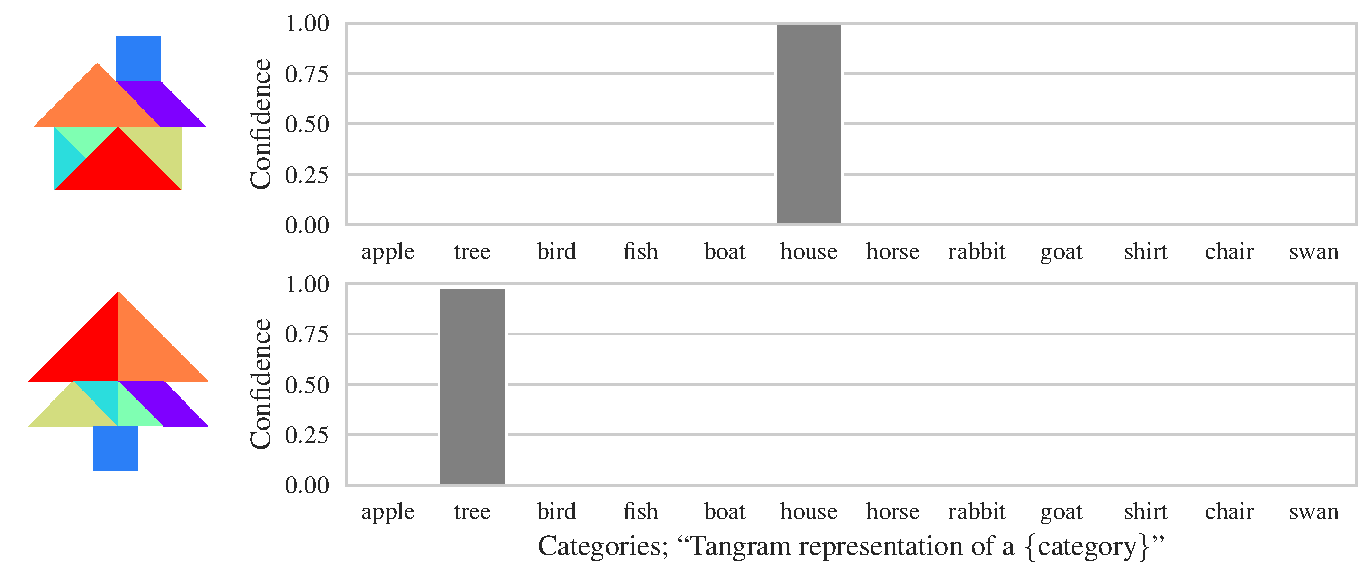
\includegraphics[width=\textwidth]{images/tangram_comparison_10.pdf}
    \caption{CLIP on a few simple Tangram creations.}
    \label{fig:clip-tangram}
\end{figure}

We did not find a significant trend in the effect of colors on the performance of CLIP, but inversions seemed to slightly affect the distribution of inferences in certain cases
(one such example is given in the appendix \figref{fig:clip-tangram-inversions}, where the distribution of CLIP was skewed in grayscale and white-on-black cases).
Consequently, we used colored or black-on-white binary renderings for our experiments.

More experiments on these hyperparameters are discussed in the later sections.


\section{Trajectory Analysis with Random Rollouts}
\label{sec:clip-problems}
% Problems with CLIP
Although we found that CLIP is quite good at recognizing these creations, we had to ensure that it would be a good source of rewards for our environments, or that the controller would be able to exploit it well to reach a sufficiently good local optimum.
To study the semantics entropy reward landscape, we conducted a series of experiments with random rollouts in the environments, i.e. starting from a meaningful creation, we perturbed the creation with randomly sampled actions and observed the effects on the reward.

These experiments showed that CLIP is quite susceptible to noise in its inferences, i.e. its probability distribution is very sensitive to small adjustments in the input image.
As a consequence of this, the reward is quite sparse, and more critically, there is a large semantic bias in not-so-meaningful images.
The sections below discuss these problems in detail.

\subsection{Sparse Rewards} % Sudden changes in rewards
\label{sec:sparse-rewards}

We observed that the inference of CLIP breaks suddenly with small changes in the image, i.e. its confidence in its classification changes very abruptly.
This results in a sparse semantics entropy reward landscape.
\figref{fig:sparse-rewards} illustrates this problem.
We destroy the image pixel by pixel using random actions left to right and see how CLIP's output changes.

\begin{figure}[h]
    \centering
    \missingfigure{Random rollouts in ShapeGridWorld.}
    \caption{Random rollouts in ShapeGridWorld.}
    \label{fig:sparse-rewards}
\end{figure}

Sparse rewards are a problem in reinforcement learning in general because underly a lack of continuous feedback. 
With only sporadic rewards, it becomes exceedingly difficult for an agent to gauge the values of actions to lead it to eventual rewards, i.e. credit assignment becomes difficult, which in turn leads to difficult and inefficient learning of action policies.

% If we imagine this scenario in reverse with an active controller, i.e. if the agent starts from the random image and tries to converge to a meaningful image by relying on the semantics entropy reward, it will have to take a series of actions that would sometimes lead to a reward and other times not.

Thus, a smooth and continuous reward is essential for effective learning.
Since we used the iCEM controller which is a gradient-free optimization algorithm and has proved to work well in sparse reward settings, we were able to circumvent this problem.

\subsection{Semantic Bias in Random Images} % Confidence in random images
\label{sec:inference-noise}
The other consequence of the noise in CLIP inference is that can sometimes confidently classify random images to a class, i.e. false positives, instead of having a flat distribution.
\figref{fig:semantic-bias-random} shows some instances of this problem where CLIP displayed high confidence in random images.

\begin{figure}[h]
    \centering
    % \includegraphics[width=0.6\textwidth]{images/p_random_semantic_bias.png}
    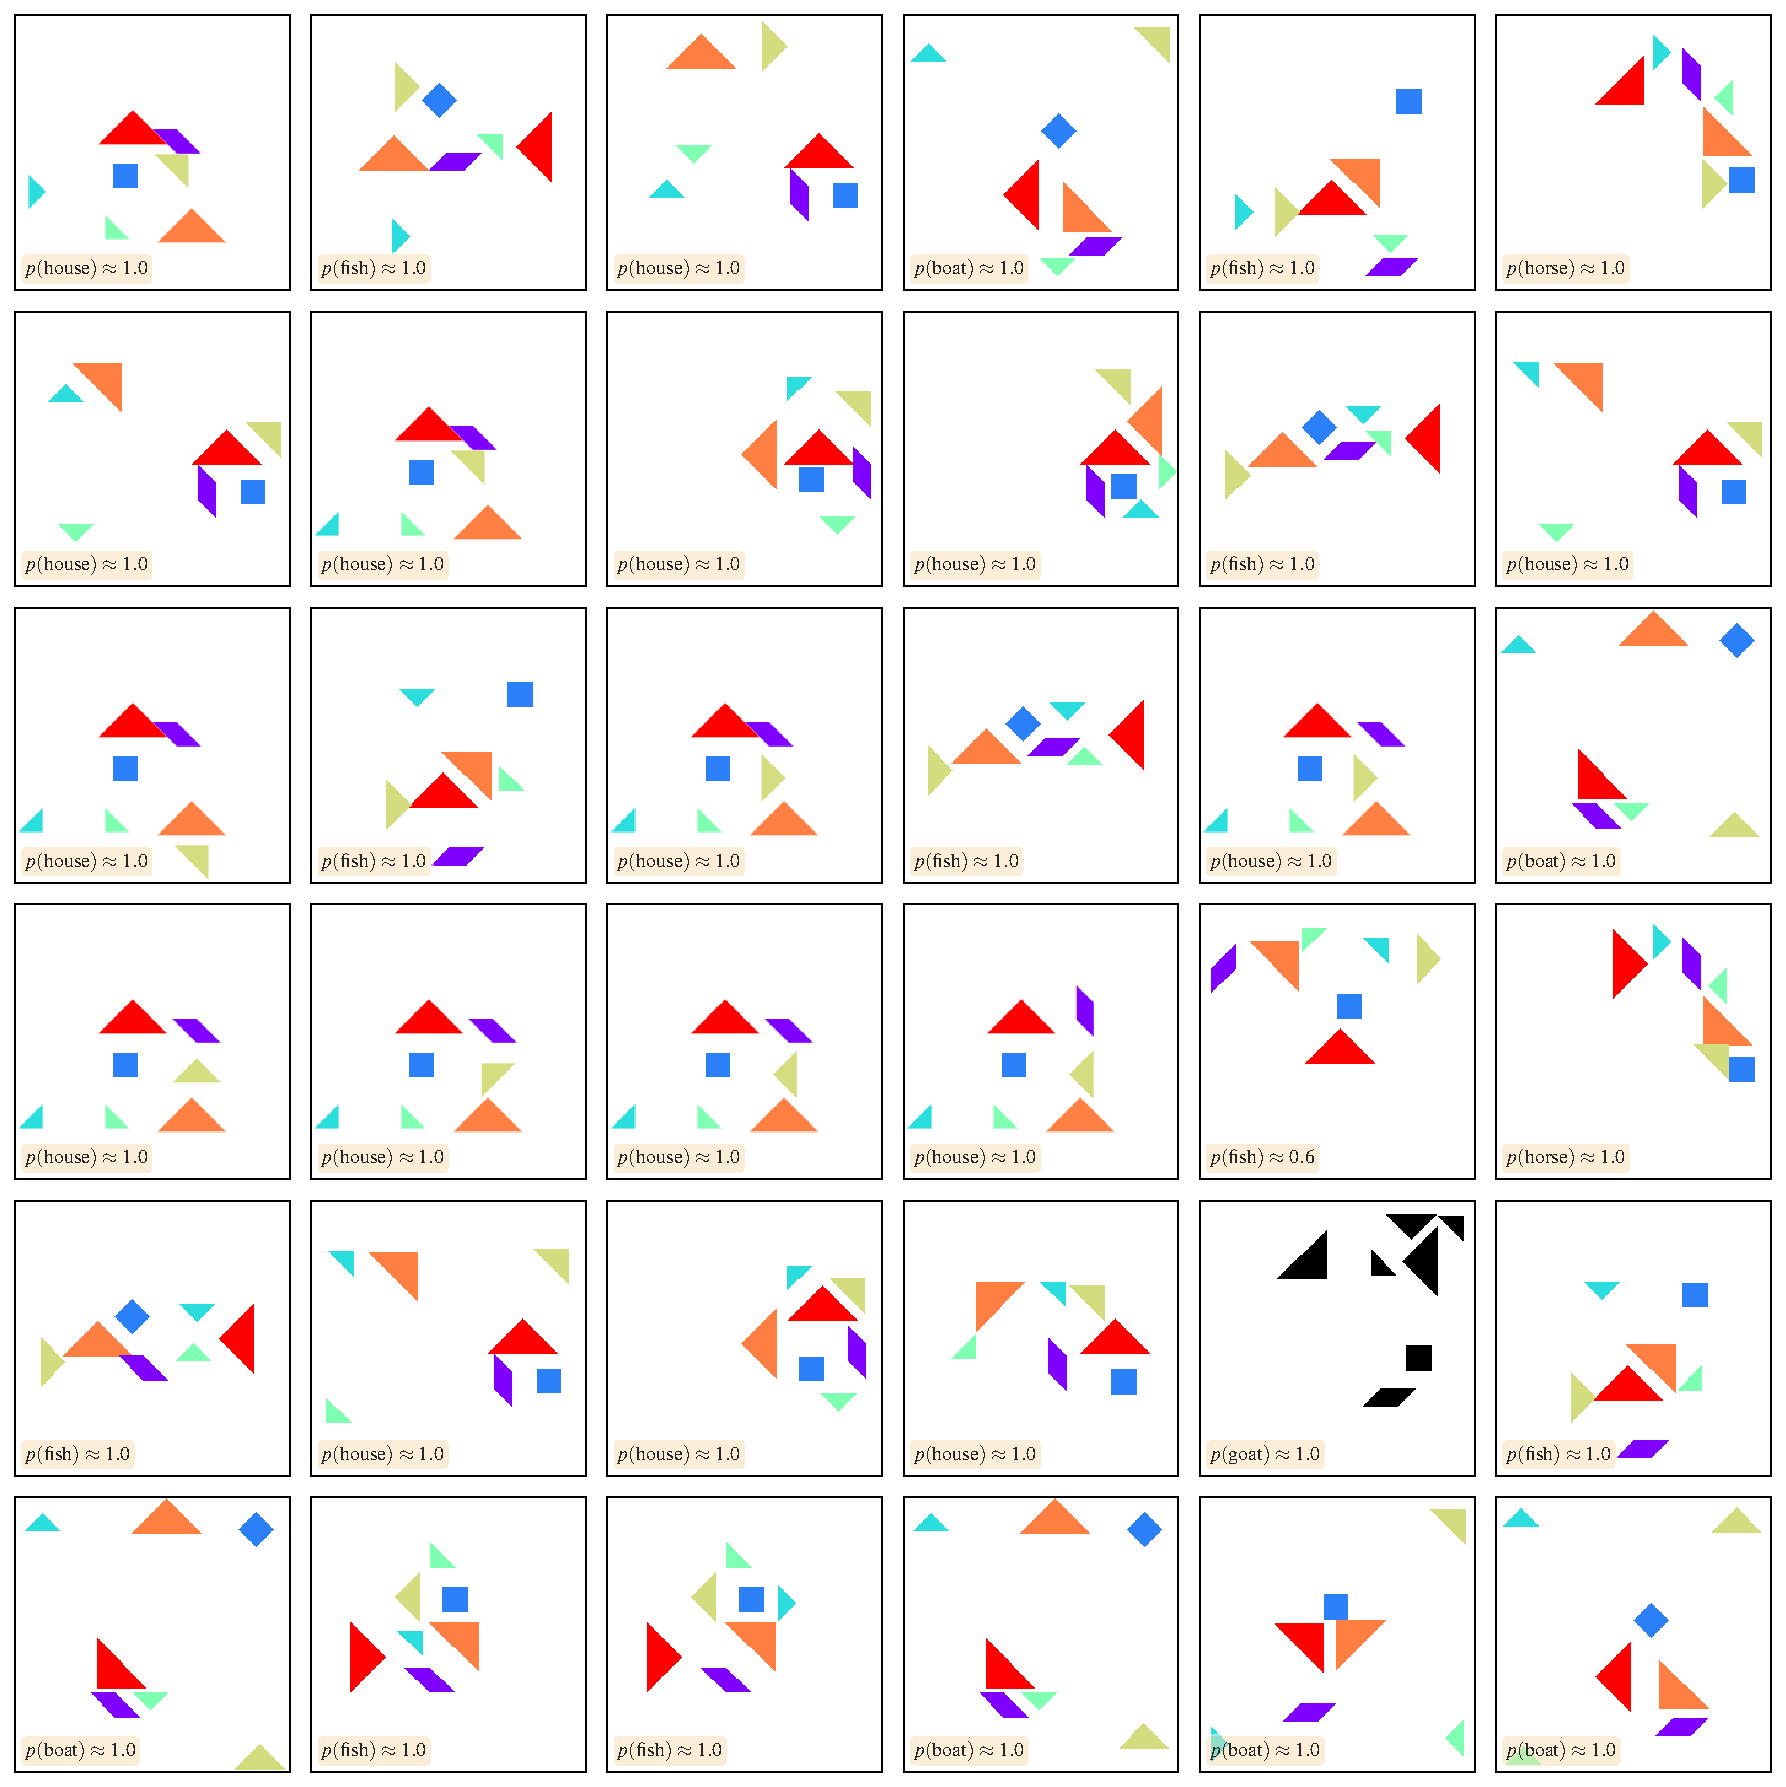
\includegraphics[width=\textwidth]{images/adversarial_samples.pdf}
    \caption{Large semantic bias in random images.}
    \label{fig:semantic-bias-random}
\end{figure}

This can also be interpreted as a jagged reward landscape with many local optima.
This noisy reward signal can lead the agent to be stuck in local optima (with a rather meaningless creation that it erroneously finds confident), or inhibit it from reaching a good optimum.

The two problems, sparse rewards and semantic bias in random images are not independent.
They have the same underlying cause -- noisy CLIP inference, yet there's a non-trivial anticorrelation between reward sparseness and noise.
That is, increasing reward density involves increasing confidence in imperfect/partial creations which also increases noise.


\subsubsection{Class Preference in CLIP}
\label{sec:class-preference}
Another complementary problem we faced related to the problem of semantic bias in random images was that of class imbalance.
Simply put, there were some classes in which CLIP was consistently more confident than others and leaned towards them over others when unsure.
This included classes that signified broad concepts like ``animal'', ``fruit'', ``number'', ``letter'', or ``object''.

% \begin{figure}[H]
%     \centering
%     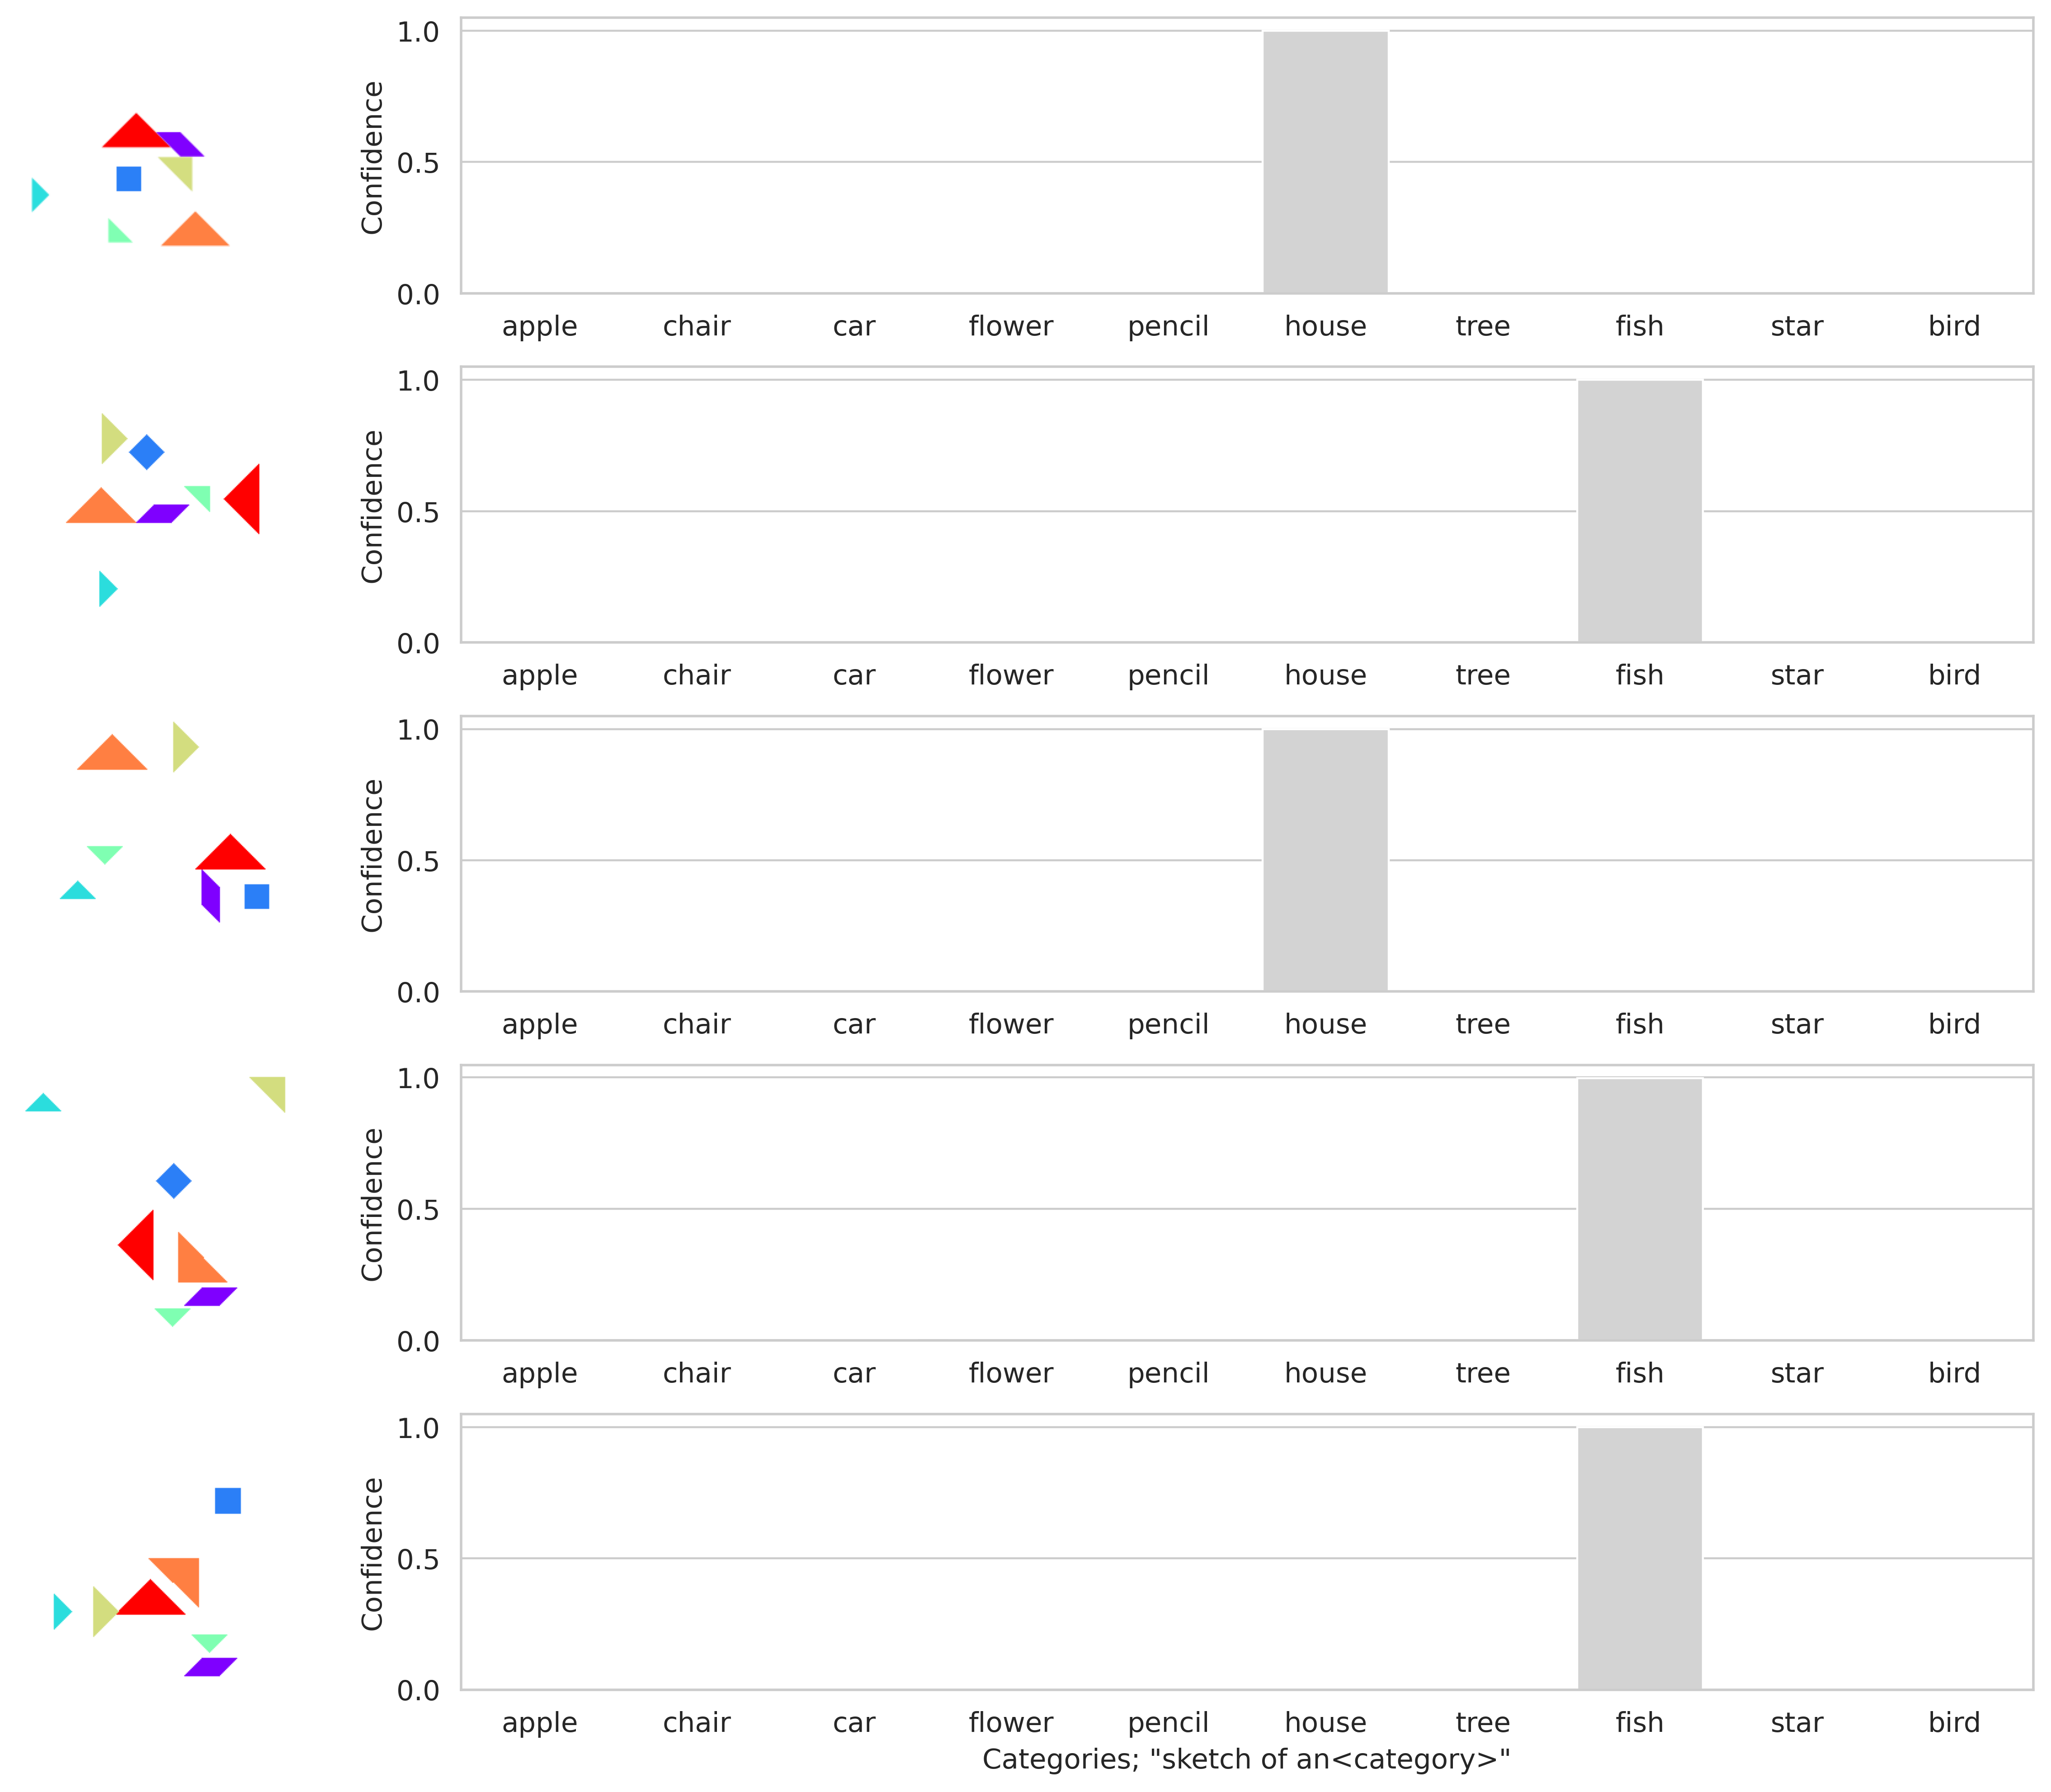
\includegraphics[width=\textwidth]{images/inference_noise.png}
%     \caption{Class preference in CLIP.}
%     \label{fig:class-preference}
% \end{figure}

This made choosing the right categories for the semantics entropy reward such that CLIP did not have a strong preference for any of them quite important.
More discussion on tackling this problem in particular is given in section \secref{sec:clip-categories}.


\section{Trajectory Analysis with Closeness Costs}
\label{sec:closeness-rollouts}
% closeness_reward_scale
% closeness_reward_threshold
Before we started improving and running simulations using inferences from CLIP, we needed to ensure that the controller was able to reach a reward-conditioned goal in our environments, i.e. it was \emph{solvable}.
Especially, it was crucial to establish this solvability under sparse rewards.

To ensure that our controller solved the environment efficiently and robustly, a good choice of the iCEM controller hyperparameters and the environment configuration was essential.
These hyperparameters and configurations were dependent on each other so we needed to optimize them together.

For example, for both environments, the size of the grid together with the step size affects the minimum required planning horizon for the controller.
For a small discrete grid or a large enough step size, the planning horizon does not need to be very high, because the controller can potentially reach the goal in a few steps and does not need to plan far ahead.
If the step size is too small for the grid size, a longer planning horizon is required so that the agent can discover the reward by random sampling.

In a similar vein, the step size is also related to the \emph{object persistency} used in the environments.
This parameter governs how many steps a single object (pixel block in ShapeGridWorld and a polygon in Tangram) is in focus for the actions of the controller before it cycles to the next object in the sequence.
For a high object persistency, the step size could be lower, but for a low object persistency, the step size needs to be higher.
(Please refer to appendix \ref{sec:icem-hyperparameters} and \ref{sec:env-hyperparameters} for more details about the hyperparameters of the iCEM controller and the environments.)

These interdependencies made the hyperparameter optimization problem quite complex and the sheer number of these parameters made this task very expensive.
Given the high computation resources and time required to run simulations with the semantics entropy reward using CLIP, it was infeasible to do a proper search over all the hyperparameters.
Thus, we instead used an alternative reward function to analyze the effect of the hyperparameters.
We called this ersatz reward function the \emph{closeness reward}.

A closeness reward is defined in the context of a fixed target creation in the environment, and its function is given as the negative of a distance function between the current creation and the target creation in the state space of the environment.

We used two different formulations of the distance function, which we called the \emph{dense closeness cost} and \emph{sparse incremental closeness cost}.
The dense closeness cost is formulated as the \(L^2\) distance between the current and target creations and the sparse incremental closeness cost is formulated as the dimension-wise thresholded \(L^1\) distance between the current and target creations, given by,
\begin{equation}
    \label{eq:closeness-reward-sparse}
    d(\bfi, \bft) = \sum_{k \in n_s} \bm{1}_\varepsilon(\bfi_k - \bft_k),
\end{equation}
where \(\bfi, \bft \in \cS\) are the current and target creations respectively, \(\varepsilon\) is a small threshold, and \(\bm{1}_\varepsilon\) is the indicator function such that \(\bm{1}_\varepsilon(x) = 1\) if \(|x| > \varepsilon\) and \(0\) otherwise.

Using the closeness reward/cost formulations, we performed an exhaustive grid search over the many hyperparameters of the iCEM controller and the environment together to find the best combinations.
The controller was able to achieve the goal under dense closeness rewards for a wide range of hyperparameters, but the tuning was more difficult under sparse incremental rewards.
Yet, we were able to find the minimal set of hyperparameters that allowed the controller to solve the environment under sparse rewards.

\begin{figure}[H]
    \centering
    \missingfigure{Closeness rollouts in Tangram.}
    \caption{Closeness rollouts in Tangram.}
    \label{fig:closeness-rollouts}
\end{figure}

To assess and compare the results of different parameters in these experiments we compared their cumulative rewards over the rollouts.

The results for the sparse incremental closeness cost on the Tangram environment are shown in \figref{fig:closeness-rollouts}.

\subsubsection{Tuning Environment Parameters}
\label{sec:env-hyperparameters}
% render_kwargs.invert
% render_kwargs.color

\label{sec:sgw-hyperparameters}
% width
% x_step
% render_delta
% object_persistency
% max_dist
% control
% control_boundaries


\label{sec:tangram-hyperparameters}
% flip
% rotate
% x_size
% r_size
% x_step
% object_persistency
% max_dist
% control
% control_boundaries
% staging_boundaries


\subsubsection{Tuning Controller Hyperparameters}
\label{sec:icem-hyperparameters}
% action_sampler_params.opt_iterations
% action_sampler_params.init_std
% action_sampler_params.elites_size
% num_simulated_trajectories
% horizon
% cost_along_trajectory
% discount_along_trajectory

\todo{Talk about the different hyperparameters that were considered. Show histograms of only the significant parameters.}


\section{Improving CLIP Rewards}
\label{sec:improving-rewards}

We experimented with several methods to reduce the noise from CLIP.
The regularized semantics reward also has many hyperparameters that can be tuned to make the reward landscape smoother.
Namely, the choice of categories/creative possibilities (\(c\)), the prefix and suffix to these categories, the temperature of the softmax function (\(T\)), the target baseline regularization strength (\(\alpha\)), the image baseline regularization strength (\(\beta\)), use of negative embeddings, and tweaking the rendering function (adding texturing or modifying the images with other operations).

The complex nature of the reward landscape and the high dimensionality of the state space made it difficult to analyze the effects of these hyperparameters.
To gain an intuition over these parameters and reduce the search space before we ran simulations using them in the full semantics reward, we instead used the best of the previously rolled-out trajectories with the closeness reward from \secref{sec:closeness-rollouts} and ran post hoc inference on the resulting sequence of image observations using CLIP and calculated the trajectories of the resulting semantics reward.
Subsequently, we performed an ablation study on these hyperparameters to gain insights into their effects \footnote{The myriad of combinations due to the high dimensional space makes it infeasible to show all the subtleties of the interplay between these hyperparameters in a few figures.
Thus, we have additionally made the analysis available for the reader as an interactive notebook at \url{https://colab.research.google.com/drive/1UzKb5t5PDRO05GbSKpgzWd3DELfAzDxJ} or \url{https://t.ly/j84on}, where one can pick a combination of different hyperparameters to see their effects}.

The following sections discuss the results of these analyses.

\subsection{Effect of the Number of Creative Possibilities}
\label{sec:clip-categories}
We found that the number of creative possibilities in the environment can also affect the performance of CLIP.
Too few categories can promote semantic bias and class preference in random images, but too many categories can exacerbate the problem of sparse rewards.
We found that the best results were obtained with a moderate number of categories (\(\sim 10\)).
This helped in mitigating the class preference in CLIP.

\begin{figure}[H]
    \centering
    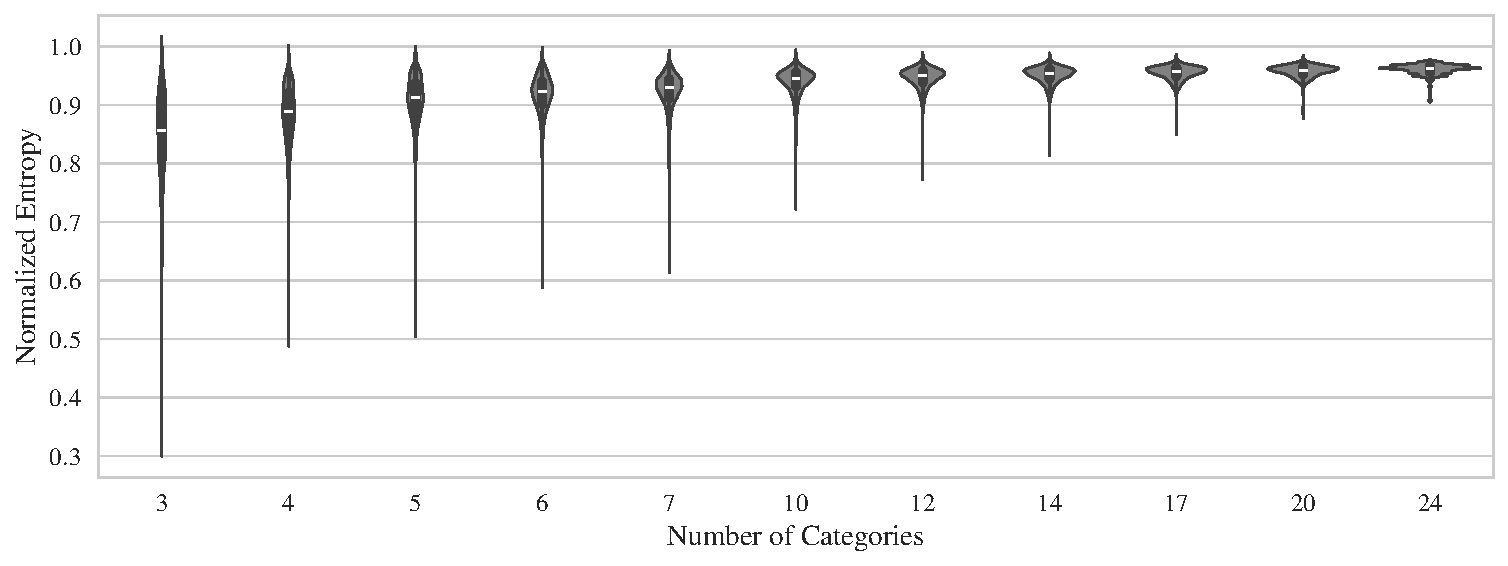
\includegraphics[width=\textwidth]{images/category_comparison_tangram.pdf}
    \caption{Effect of the number of categories on CLIP inference distribution over a random image.}
    \label{fig:clip-categories}
\end{figure}

\subsection{Effect of Temperature}
\label{sec:reg-temperature}
% semantics_model_temperature
\begin{figure}[H]
    \centering
    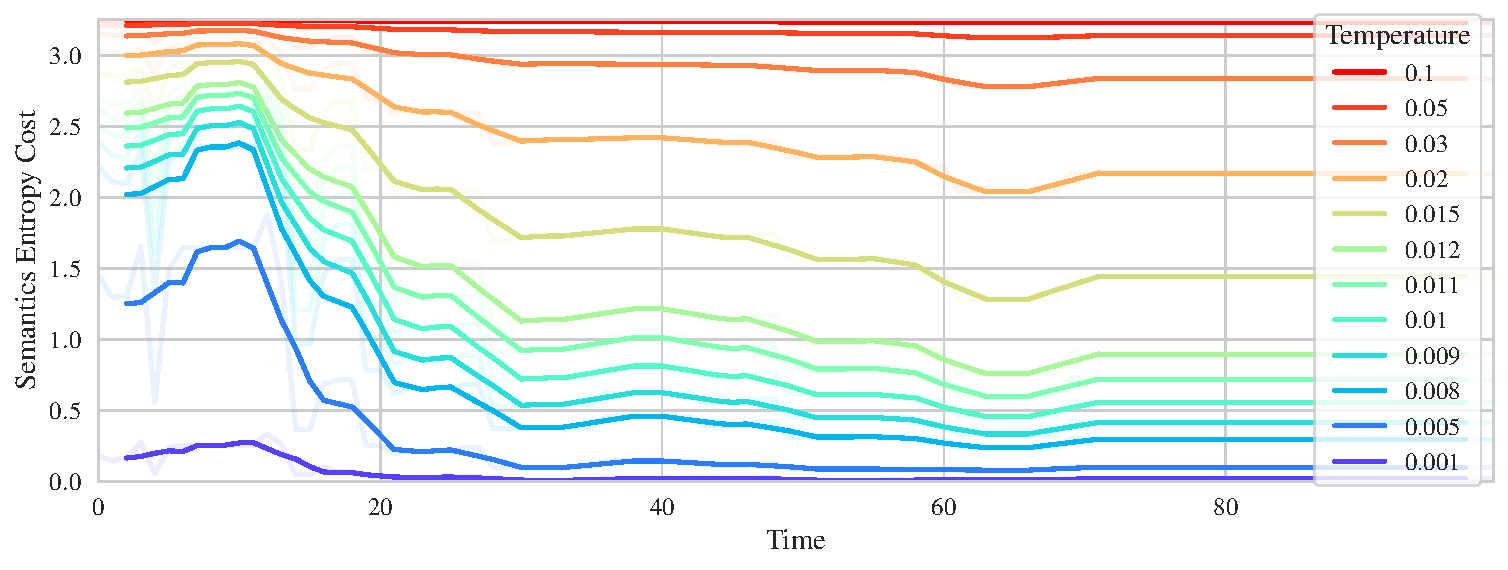
\includegraphics[width=\textwidth]{images/temperature_comparison.pdf}
    \caption{Effect of temperature on semantics entropy reward trajectories.}
    \label{fig:clip-temperature}    
\end{figure}

\subsection{Effect of Target Baseline Regularization}
\label{sec:reg-alpha}
% semantics_alpha_target


\subsection{Effect of Image Baseline Regularization}
\label{sec:reg-beta}
% semantics_beta_image

\begin{figure}[H]
    \centering
    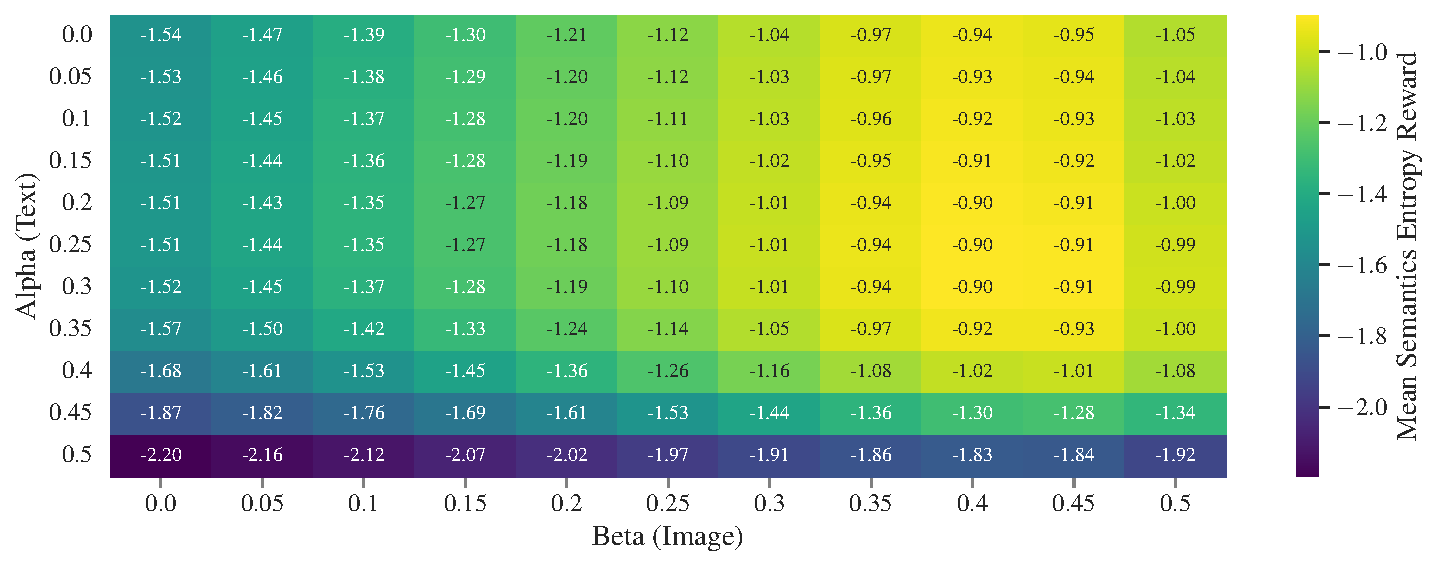
\includegraphics[width=\textwidth]{images/alpha_beta_temp12avg_noneg.pdf}
    \caption{Effect of regularization strength on semantics entropy reward trajectories.}
    \label{fig:clip-alpha-beta}
\end{figure}


% \subsection{Effect of Changing Prefix and Suffix}
% \label{sec:prefix-suffix}
% % label_prefix
% % label_suffix
% Different prefixes/suffixes and combinations of them also affected the performance of CLIP.

% \begin{figure}[H]
%     \centering
%     \missingfigure{Effect of changing the prefix suffix.}
%     \caption{Effect of different prefixes and suffixes.}
%     \label{fig:prefix-suffix}
% \end{figure}

\subsection{Effect of Adding Post-Suffix}
\label{sec:post-suffix}
Following the insights from \cite{waffleclip}, we also experimented with adding concepts and/or a random string of jibberish to the end of the label as a \emph{post-}suffix to see if it affected the reward. 

While it did affect the reward, the effect was not significant, and we could not realize the exact mechanism for choosing a post-suffix that would work well in general.

\begin{figure}[H]
    \centering
    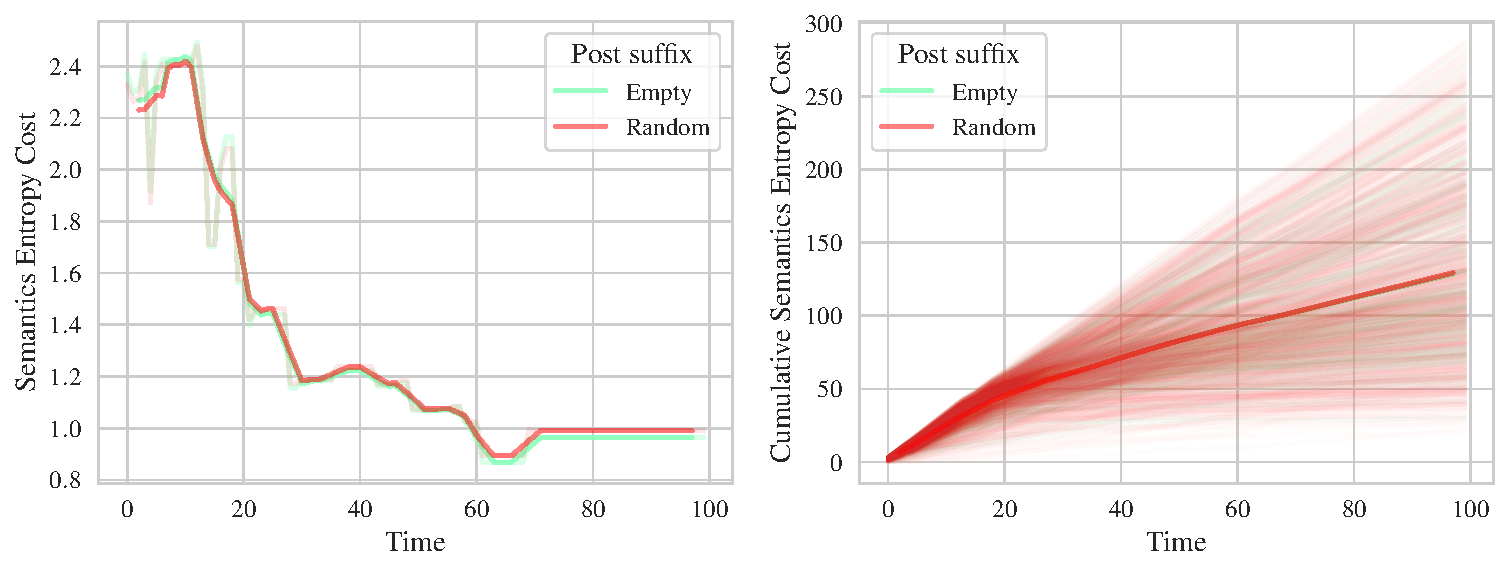
\includegraphics[width=\textwidth]{images/post_suffix_comparison.pdf}
    \caption{Effect of different post-suffixes on semantics entropy reward trajectories.}
    \label{fig:post-suffix}
\end{figure}


\subsection{Effect of Negative Embeddings}
\label{sec:negative-embeddings}
\cite{negprompt} used negative embeddings in their goal-conditioned CLIP reward function to make the reward landscape smoother.
We experimented with this as well, and instead of using the initial description of the environment as the text baseline, we used a negative embedding of the target creation.

We did not find this to be helpful in our experiments, instead it seemed to flatten the reward landscape.
We think this is a consequence of CLIP's language encoder being a bag-of-words model, and the negative embeddings being essentially close to the target embeddings, which effectively zeros out the target embeddings.

\begin{figure}[H]
    \centering
    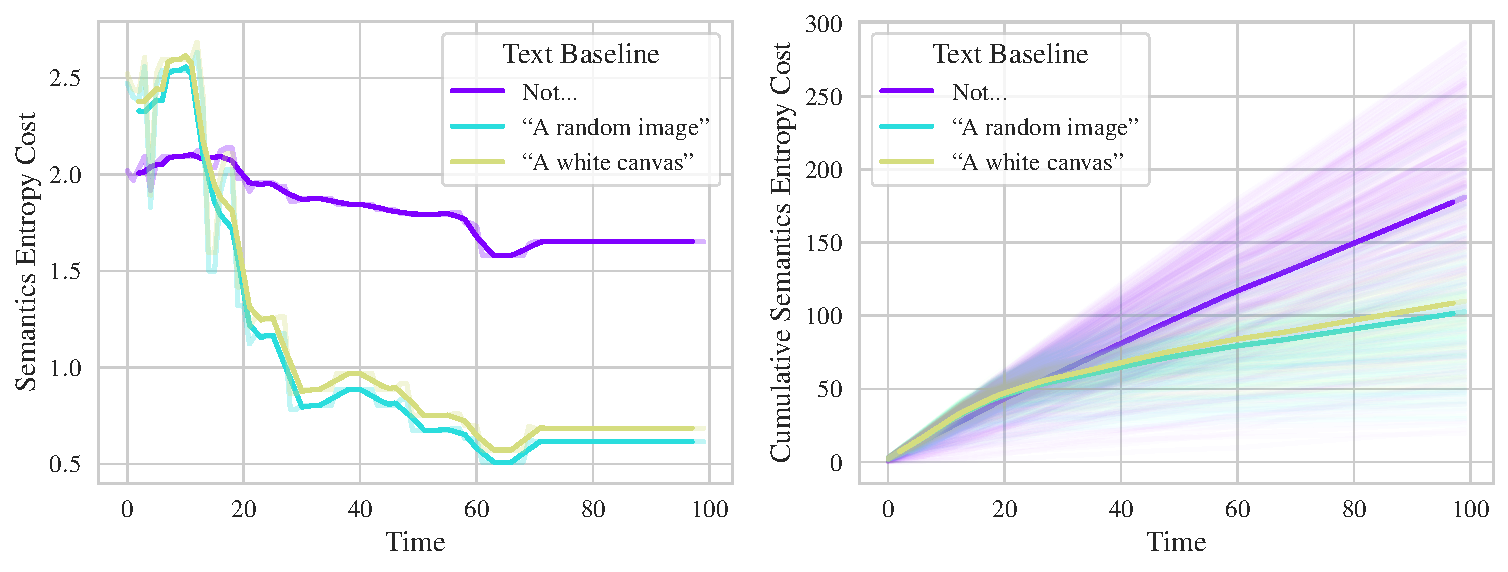
\includegraphics[width=\textwidth]{images/baseline_comparison.pdf}
    \caption{Effect of different text baselines on semantics entropy reward trajectories.}
    \label{fig:baseline}
\end{figure}

\subsection{Effect of Image Texturing}
\label{sec:image-texturing}
Following the observations from \cite{vlmrm}, we also experimented with adding textures to the images to make them more realistic for CLIP in hopes of improving its quality.


\subsection{Effect of Image Operations}
\label{sec:image-operations}
% Shearing and Hatching
We also had the idea to use image operations like shearing and rotation before inference.
We expected the true positive semantic inferences to be invariant to these operations, but the false positives to be reduced.

While rotating did not have a significant effect, we found that shearing the images before inference did improve the quality of the inferences slightly.

\begin{figure}[H]
    \centering
    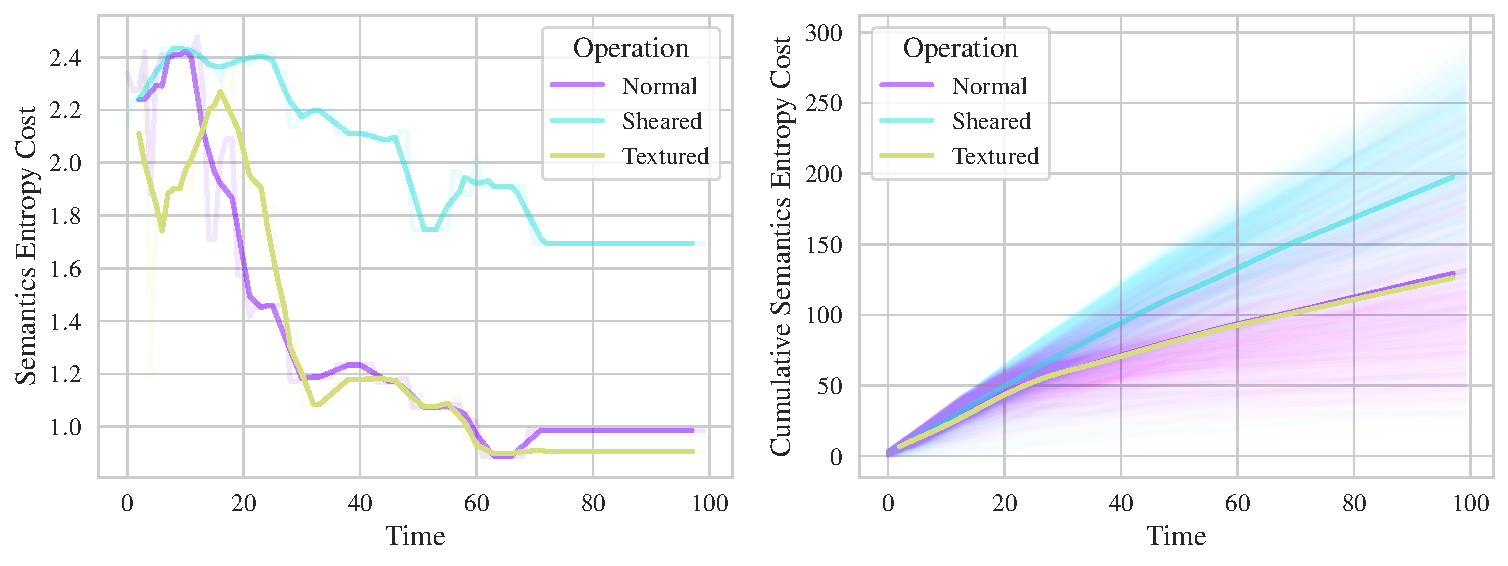
\includegraphics[width=\textwidth]{images/texturing_operations_comparison.pdf}
    \caption{Effect of texturing and image operations on semantics entropy reward trajectories.}
    \label{fig:texturing-operations}
\end{figure}

% \begin{figure}[H]
%     \centering
%     \missingfigure{As a consolidation of everything before, a bar plot with ablations.}
%     \caption{Ablations of the different methods to improve semantics entropy reward.}
%     \label{fig:clip-ablation}
% \end{figure}


\subsection{Entropy Regularization}
\label{sec:entropy-regularization}
Another promising way to make the reward landscape of CLIP smoother is to fine-tune it with an additional entropy regularization loss over its output.
This is given by,
\begin{equation}
    \label{eq:entropy-regularization}
    L(\bmi, \bml) = L_{\iota}(\bmi, \bml) \underbrace{- \sum_{\bfi_k \in \bmi}\sum_{\bfl_j \in \bml} p(\bfl_j; \bfi_k, \bml) \log p(\bfl_j; \bfi_k, \bml)}_{\text{Entropy Regularization}},\\
\end{equation}
where \(L_{\iota}\) is the contrastive cosine-similarity loss used to train CLIP and \(p(\bfi_k, \bml)\) is the classification probability distribution of image \(\bfi_k\) over the labels \(\bml\) predicted by CLIP.

We experimented with this regularization method on a toy convolutional neural network (CNN) for classifying handwritten digits, which we called \emph{Flatnet}.
We found it to be quite effective in smoothing the reward landscape.
Both our problems from \secref{sec:clip-problems} were relieved -- the reward trajectory was smoother and we observed less semantic bias in random images.

Yet, we did not use it to fine-tune CLIP to limit the scope of the project given the limited time.
The results of this analysis can be found in appendix \ref{sec:flatnet}.

\subsection{Adversarial Performance}
\label{sec:adversarial-performance}
To tackle the problem of semantic bias in random images, we collected samples of the false positive image observations from our rollouts, called \emph{adversarial observations}, by filtering out the image observations with low entropy from all our runs and then manually removing the ones that were true positives.
Then, we searched for the semantics reward regularization hyperparameters that would decrease its specificity while maintaining its sensitivity, i.e. make CLIP less confident in the adversarial images while maintaining its inference for the truly semantically expressive images.

\begin{figure}[H]
    \centering
    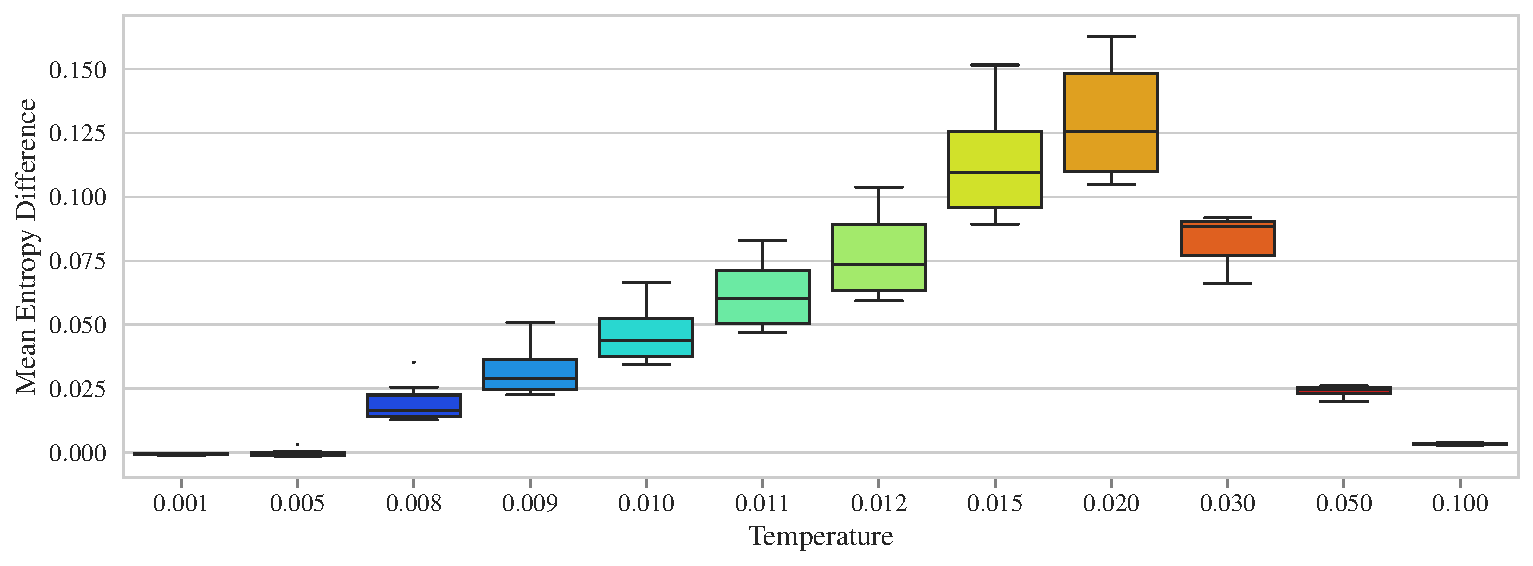
\includegraphics[width=\textwidth]{images/temperature_adversarial.pdf}
    \caption{Effect of temperature on discerning true positives from false positives.}
    \label{fig:clip-temperature-adversarial}
\end{figure}

\begin{figure}[H]
    \centering
    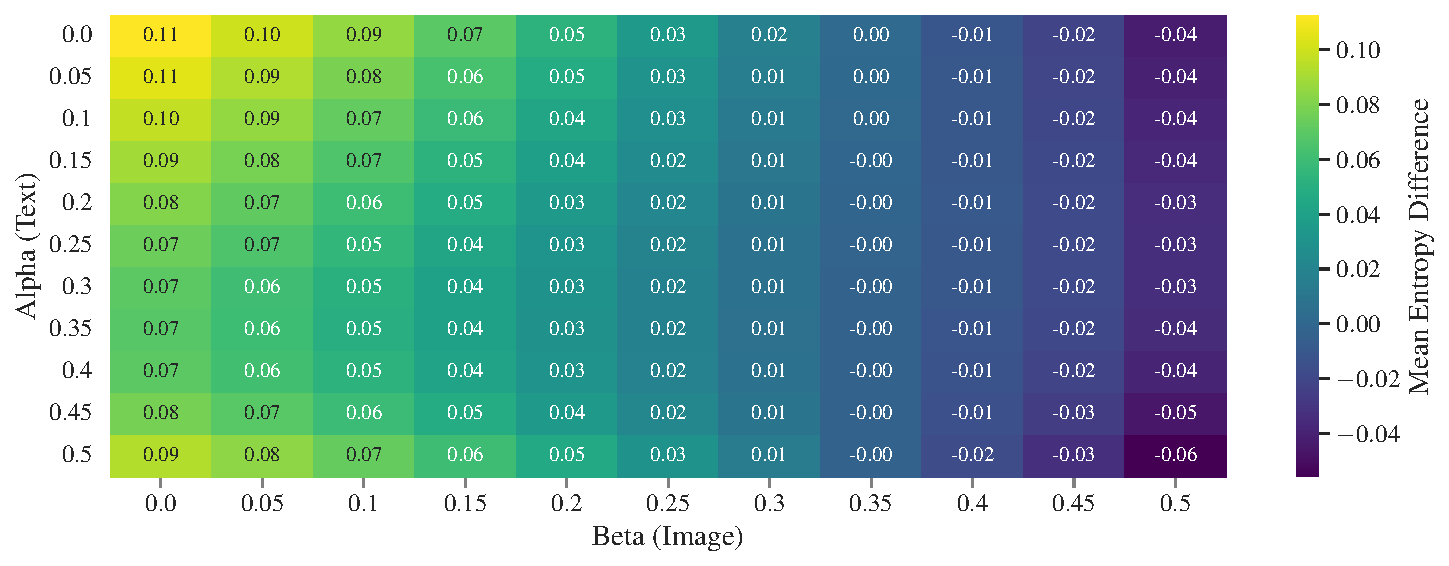
\includegraphics[width=\textwidth]{images/alpha_beta_adversarial.pdf}
    \caption{Effect of regularization strength on discerning true positives from false positives.}
    \label{fig:clip-alpha-beta-adversarial}
\end{figure}

\begin{figure}[H]
    \centering
    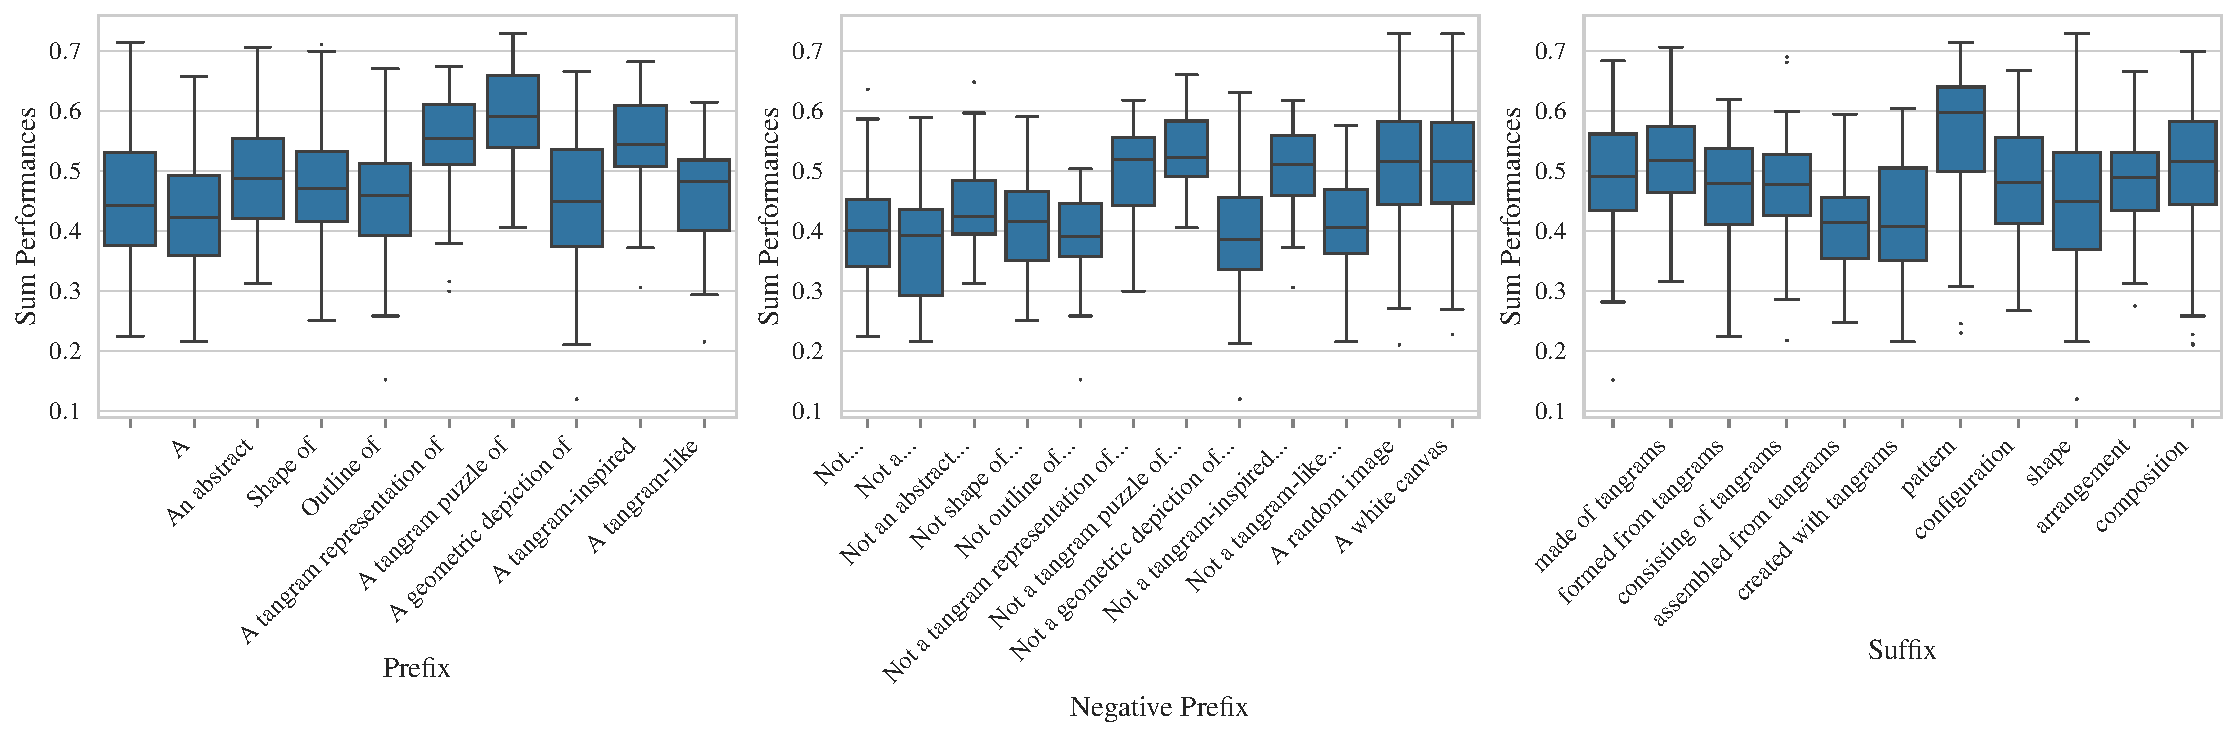
\includegraphics[width=\textwidth]{images/post-suffix_adversarial.pdf}
    \caption{Effect of different post-suffixes on discerning true positives from false positives.}
    \label{fig:post-suffix-adversarial}
\end{figure}

\begin{figure}[H]
    \centering
    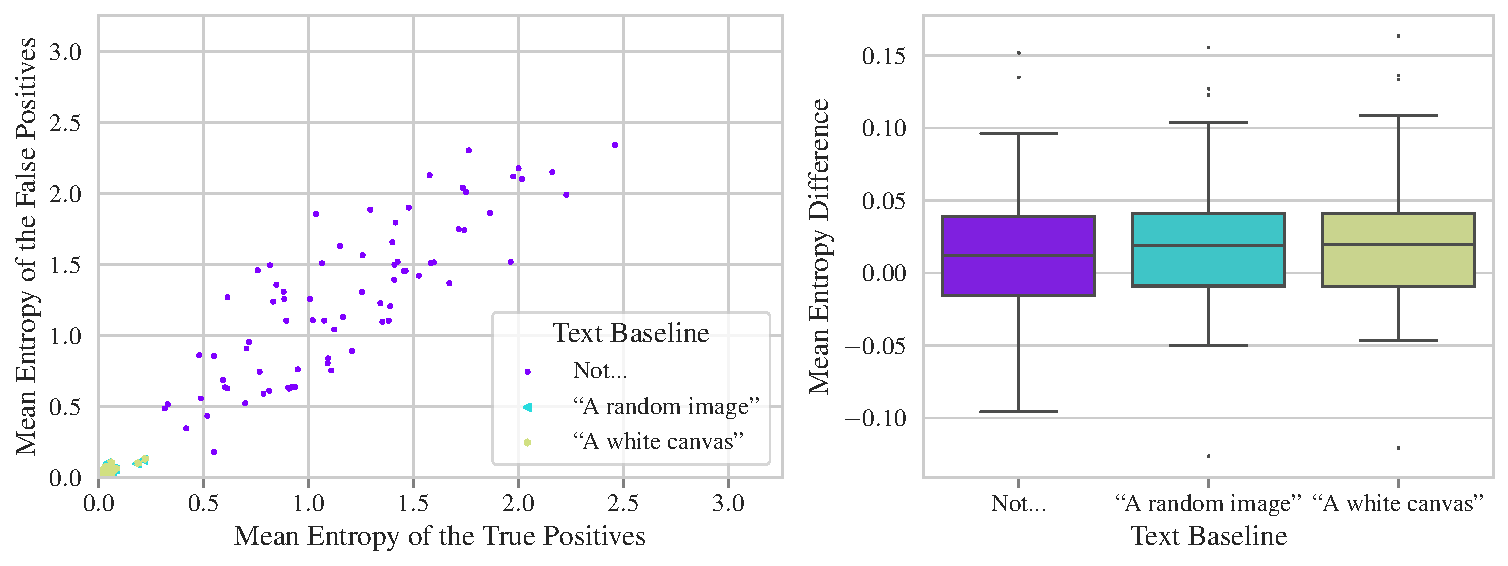
\includegraphics[width=\textwidth]{images/baseline_adversarial.pdf}
    \caption{Effect of different text baselines on discerning true positives from false positives.}
    \label{fig:baseline-adversarial}
\end{figure}

\begin{figure}[H]
    \centering
    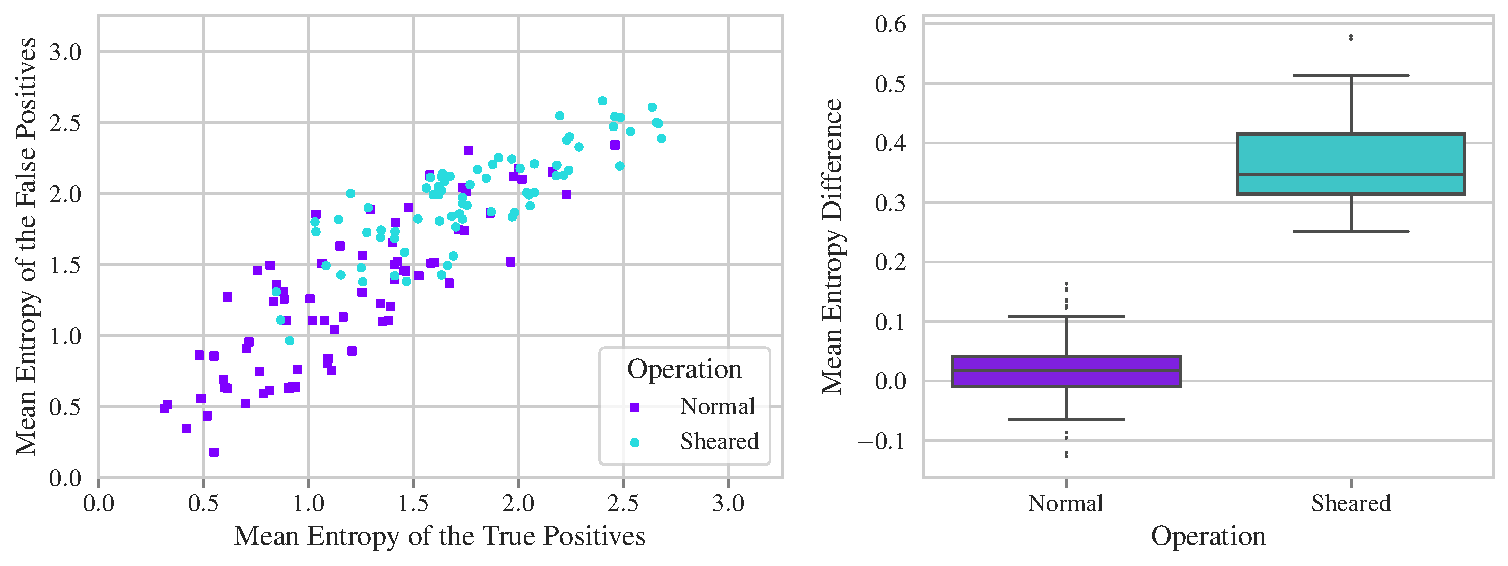
\includegraphics[width=\textwidth]{images/texturing-operations_adversarial.pdf}
    \caption{Effect of image operations on discerning true positives from false positives.}
    \label{fig:texturing-operations-adversarial}
\end{figure}

% \figref{fig:adversarial-images} shows the results of our analysis.
% \begin{figure}[H]
%     \centering
%     \includegraphics[width=\textwidth]{images/p_adversarial_histogram.png}
%     \caption{Effect of different prefixes and suffixes.}
%     \label{fig:prefix-suffix-adversarial}
% \end{figure}

By choosing the right hyperparameters for the semantics reward, we were able to improve the predictive value of CLIP for our environments.

\newpage
\section{Simulations}
\label{sec:simulations}
% Manual ranking and entropy ranking

Once we had found suitable combinations of the controller and environment hyperparameters, and had developed an intuition of the semantics entropy reward hyperparameters, we finally ran simulations with the semantics reward to generate creations in the environments.

To evaluate these creations, in addition to the cumulative reward, we also asked two human evaluators to manually rank the final creations on a scale of \(1\) to \(5\) based on their apparent semantic expressiveness.

% \subsection{Evaluating Regularized Entropy Reward Formulation in Goal-Conditioned Tasks}
% \label{sec:evaluating-regularized-entropy}
% % alpha_target
% % beta_image


% What makes CLIP think that the creation is a certain class?
% - Apple with the red and the green/yellow triangle
% - Hammer with the parallelogram and the square
% - Heart with the red triangle pointing down
% - House with a triangle and the square



\subsection{Effect of RaIR}
\label{sec:effect-rair}
% compression_precision
% 1 / semantics_reward_scale

The additional structural bias helped with grounding and coalescing the creations in more human-recognizable forms and patterns.


\subsection{Partial Completions on ShapeGridWorld}
\label{sec:partial-completion}

% The Discussion should begin with a statement of the important findings of the study. Subsequent sections can address technical issues, analysis of the results, and the implications of the work. Again, it is often helpful to break down the Discussion into subsections that focus on particular topics. It is proper to include a section that summarizes and expands upon conclusions that may be drawn from the work (raises open questions, proposes future studies).
\chapter{Discussion}
\label{sec:discussion}

% Summary of CLIP reward analysis

% Limitations
% - CLIP is noisy
% - Should/Could improve with better models
We did not get major performance improvements with additional prompt engineering and hyperparameter tuning.
We think that these failures are related to capability limitations in the CLIP model we use.
This is similar to the findings observed by \cite{vlmrm} in their use of CLIP as a source of goal-conditioned rewards.

\todo{Summary of things. Things that could be helpful.}

% Comments on regularization

% RaIR was very helpful
We observed that the complementary RaIR reward was very helpful in improving the quality of the semantics reward.
It helped with grounding and coalescing the structures in more human-recognizable forms and patterns.

% Comments on the environments

% Future work
Perhaps using bigger models from OpenCLIP such as \texttt{ViT-bigG-14} \citep{openclip} which are trained on the LAION-5B dataset \citep{laion5b} might lead to some performance improvements.

% Comments on creativity

% Comments on exploration
When used as an additional reward to augment traditional novelty-seeking intrinsic rewards \(r_{\text{intrinsic}} = r_{\text{semantics}} + r_{\text{novelty}}\), it can lead to more human-like exploration i.e. curious behaviors with semantically-sound creative expression.

\pagestyle{plain}
% These may include thanks to technicians or colleagues who have helped with the work or provided materials.
\section{Acknowledgements}

I would like to express my deepest gratitude to my supervisor Cansu Sancaktar for her patience, guidance, and motivation throughout the project.\\\vspace{-12pt}

I would also like to thank Georg Martius for giving me this opportunity. And to the Graduate Training Center for Neuroscience for their support.\\\vspace{-12pt}

Lastly, I thank my family, especially my parents, and my friends and classmates, for their intellectual and moral inspiration.

% All references cited in the text (and only those cited in the text) should be included. References in the text should be cited by author’s name and year of publication (Kandel, 2002, Hodgkin and Huxley, 1952, Zigmond et al., 2000a, b). Only published and “in press” (i.e., accepted for publication) references should appear in the reference list (in alphabetical order by author, then chronological order by year). A standard format of listing references looks like this: Hodgkin AL, Huxley AF (1952) The components of membrane conductance in the giant axon of Loligo. J Physiol (Lond) 116:473-496. 
% \markboth{}{}
\renewcommand{\bibname}{References}
\bibliographystyle{apalike}
\bibliography{ref_strings.bib, ref.bib}

\begin{appendices}    
\makeatletter
\addtocontents{toc}{\let\protect\l@chapter\protect\l@section}
\addtocontents{toc}{\let\protect\l@section\protect\l@subsection}
\makeatother
\addtocontents{toc}{\protect\setcounter{tocdepth}{1}}
\addtocontents{lof}{\protect\pagebreak}

\chapter{Environments' Details}
\label{sec:environments-details}
The sections of this chapter provide additional details about the custom environments used in our experiments.
Both of these environments are developed in Python.

\section{ShapeGridWorld}
\label{sec:sgw-details}
% Added color
% Added object_persistency 0
% Added step_size > 1
% Improved rendering
% Added partial reset with control and control boundaries
% Added controlled reset with max_dist
% Added partial control with control and control boundaries
\tabref{tab:original-sgw-params} lists the parameters of the original ShapeGridWorld environment developed by \cite{rair}, along with the best values we found for our experiments.
\begin{table}[H]
    \centering
    \caption{Original ShapeGridWorld parameters.}
    \begin{tabularx}{\textwidth}{C{3.9cm} L C{2cm}}
        \hline
        Property & Description & Best/(Default)\\
        \hline
        \texttt{width} & Width of the discrete grid. & \(28\)\\
        \texttt{height} & Height of the discrete grid. Kept same as \texttt{width}. & \(28\)\\
        \texttt{n\_pixels} & Number of ``On'' pixels, \(n_e\). & \(\sim 20\)\\
        \texttt{shape} & Shape of a pixel block. & (``circle'')\\
        \texttt{size} & Size of a pixel block. & \(7\)\\
        \texttt{persistency} & Number of time steps an object (pixel block) is moved. & \(1\)\\
        \hline
    \end{tabularx}
    \label{tab:original-sgw-params}
\end{table}
The state space of this environment is composed of the \(x\) and \(y\) coordinates of the \(n_e\) block pixels, with the addition of two dimensions for the state space of the agent -- one that specifies which object is currently in focus and another that specifies how many times it has already moved, i.e. \(\cS \in \nN^{2 n_e + 2}\).
The observation space is a rendering of the grid as an image of shape \(\texttt{width} * \texttt{size} \times \texttt{height} * \texttt{size}\).

The action space comprises the action value for each of the directions (x and y) for an object; \(\cA \in [-1, 1]^{2 n_e}\).
For each dimension, the controller samples from a continuous distribution in \([-1, 1]\), which is uniformly mapped to \(\{-1, 0, 1\}\) (\([-1, -1/3) \mapsto -1, [-1/3, 1/3] \mapsto 0, (1/3, 1] \mapsto 1\)).

We further added more features to this environment for our experiments, which are listed in \tabref{tab:additional-sgw-params}.
In particular, the ability to move all objects at once and more than one step in an action step was added.
We also developed a controlled reset method with the added feature to freeze sections of the grid, with \texttt{control} and \texttt{control\_boundaries}.
This additionally enabled us to allow the controller only partial access to the environment.
Furthermore, the rendering function was reimplemented using faster methods from \emph{OpenCV}; see \secref{sec:improving-render} for more details.

\begin{table}[H]
    \centering
    \caption{Additional ShapeGridWorld parameters.}
    \begin{tabularx}{\textwidth}{C{3.9cm} L C{2cm}}
        \hline
        Property & Description & Best/(Default)\\
        \hline
        \texttt{step\_x} & Maximum number of steps an object can be translated in the x-direction in one action. & \(7\)\\
        \texttt{step\_y} & Maximum number of steps an object can be translated in the y-direction in one action. Kept same as \texttt{step\_x}. & \(7\)\\
        \texttt{persistency*} & Added the ability to move all objects at once. & \(1\)\\
        \texttt{color} & A flag to enable grayscale values for pixels. & False\\
        \texttt{invert} & A flag to control the inversion of the rendered images.  & True\\
        \texttt{control\_boundaries} & If specified, objects inside these limits \emph{initially} are marked. & (None)\\
        \texttt{control} & A flag to define the scope of control, i.e. whether all the objects or only those marked initially by the control boundaries can be moved. & (``all'')\\
        \texttt{max\_reset\_dist} & Maximum distance an object can be moved from its original position on reset. Only the objects marked initially are reset. There are no constraints if set to \(-1\). & (\(5\))\\
        \hline
    \end{tabularx}
    \label{tab:additional-sgw-params}
\end{table}

If all objects are moved at once, the state space of this environment is composed of only the \(x\) and \(y\) coordinates of the block pixels, i.e. \(\cS \in \nN^{2 n_e}\).
The corresponding action space in this case would be \(\cA \in [-1, 1]^{2 n_e}\).
For each dimension of the action space, the controller samples from a continuous distribution in \([-1, 1]\), which is uniformly mapped to integers \([-l, l]\), where \(l \in \{\texttt{step\_x}, \texttt{step\_y}\}\) is the step size of the dimension.

\subsection{ShapeGridWorld Image Registration Technique}
\label{sec:sgw-registration}

To test CLIP inference on ShapeGridWorld and simulate the controller on partial drawings, without having to draw these drawing samples manually, a registration method for images was developed that reads a given image to generate a corresponding ShapeGridWorld of given dimensions.

This is done using a circular convolution kernel over the image to find the corresponding grid pixel values.
Optionally, it makes the lines in the image thinner by finding its skeleton using morphological operations before the convolution.
See \figref{fig:sgw-registration} for a demonstration.

% \vspace{12pt}
\begin{figure}[H]
    \centering
    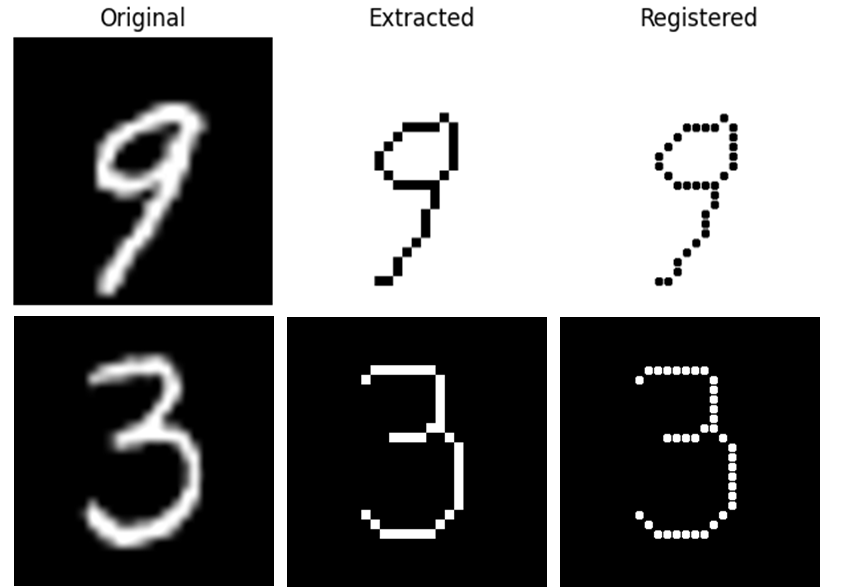
\includegraphics[width=0.66\textwidth]{images/grid_registration.png}
    \caption{ShapeGridWorld image registration on images from the MNIST dataset.}
    \label{fig:sgw-registration}
\end{figure}
% \vspace{12pt}

We developed a wrapper around the PIL Python library \citep{pil} to conveniently perform these operations and generate ShapeGridWorld environments.
The relevant code is hosted on \url{https://github.com/pulkitgoyal56/ImageGrid}.
\tabref{tab:imagelib-params} lists the relevant parameters of this image registration library, along with the default values.
\begin{table}[H]
    \centering
    \caption{Image registration parameters.}
    \begin{tabularx}{\textwidth}{C{3.9cm} L C{2cm}}
        \hline
        Property & Description & Default\\
        \hline
        \texttt{mode} & PIL Image mode in which the image is read. & ``1'' (Binary)\\
        \texttt{invert} & A flag to control the inversion of the read image. The expected image should be white on black. & False \\
        \texttt{threshold\_ratio} & Threshold on the convolution sum, for binary grids. & \(0\)\\
        \hline
    \end{tabularx}
    \label{tab:imagelib-params}
\end{table}

\section{Tangram}
\label{sec:tangram-details}
% flip
% rotate
% x_size
% r_size
% x_step
% object_persistency
% max_dist
% control
% control_boundaries
% staging_boundaries

The Tangram environment is constructed with a list of polygon objects created using the provided \texttt{Polygon} class, which defines a polygon's size, shape, and color.
The additional parameters of the Tangram environment are tabulated in table \tabref{tab:tangram-params}.
\begin{table}[H]
    \centering
    \caption{Tangram parameters.}
    \begin{tabularx}{\textwidth}{C{3.9cm} L C{2cm}}
        \hline
        Property & Description & Best/(Default)\\
        \hline
        \texttt{x\_size, y\_size} & Span of the discrete grid; number of steps in the x and y directions. If set to \(1\), grid is continuous in \([0, 1]\). & \(1\)\\
        \texttt{x\_step, y\_step} & Maximum number of steps a polygon can be translated in the x and y directions in one action. & \(5\)\\
        \texttt{r\_size} & Span of the discrete grid; number of rotation steps in \(180^\circ\). If set to \(1\), rotation is continuous in \([0, 180^\circ]\). & \(1\)\\
        \texttt{r\_step} & Maximum number of steps a polygon can be rotated in one action. & \(4\)\\
        \texttt{rotate} & A flag to enable/disable rotation. & True\\
        \texttt{flip} & A flag to enable/disable flipping. & False\\
        \texttt{persistency} & Number of time steps a polygon (pixel block) is moved. If set to \(1\), all polygons are moved at once. & \(1\)\\
        \texttt{control\_boundaries} & If specified, polygons inside these limits \emph{initially} are marked. & (None)\\
        \texttt{control\_criteria} & The point inside the polygon that determines if the polygon is inside or outside the control boundaries. A Python lambda function or an attribute of \texttt{Polygon}, such as ``centroid'' for the centroid, ``center'' for the mean of the vertices, or ``complete'' for the entire polygon. & (``center'')\\
        \texttt{control} & A flag to define the scope of control, i.e. whether all the polygons or only those marked initially by the control boundaries can be moved. & (``all'')\\
        \texttt{staging\_boundaries} & If specified, only polygons inside these limits are rendered to get a state's corresponding image observation. See \figref{fig:staging-boundaries} & None\\
        \texttt{staging\_criteria} & Like \texttt{control\_criteria} but for staging boundaries. & (``complete'')\\
        \texttt{max\_reset\_dist} & Maximum distance a polygon can be moved from its original position on reset. Only the polygons marked initially are reset. There are no constraints if set to \(-1\). & (\(-1\))\\
        \hline
    \end{tabularx}
    \label{tab:tangram-params}
\end{table}

The state space of this environment is composed of the \(x\) and \(y\) coordinates of the vertices of the \(n_e = 7\) polygons, with the addition of two dimensions for the state space of the agent -- one that specifies which polygon is currently in focus and another that specifies how many times it has already moved, i.e. \(\cS \in \nN^{\,2 + \sum_{i \in n_e} 2\ N_v(p_i)}\), where \(N_v(p_i)\) is the number of vertices of polygon \(p_i\).
If all polygons are moved at once, the state space of this environment is composed of only the \(x\) and \(y\) coordinates of the block pixels, i.e. \(\cS \in \nN^{\sum_{i \in n_e} 2\ N_v(p_i)}\).
The observation space is a rendering of the grid whose resolution is controlled with different parameters.

The action space comprises the action value for each of the degrees of freedom (x, y, rotation, and flip) for an object; \(\cA \in [-1, 1]^4\).
For each dimension of the action space, the controller samples from a continuous distribution in \([-1, 1]\).
In the x-, y-, and rotation dimensions, this is uniformly mapped to integers in \([-l, l]\), where \(l \in \{\texttt{step\_x}, \texttt{step\_y}, \texttt{step\_r}\}\) is the step size of the dimension, if it is discrete.
If the dimension is continuous (because its \texttt{size} is set to \(1\)), the action is scaled by its respective step size instead.
The \texttt{step} parameter can then be understood as the minimum number of actions required to move a polygon across the entire grid.
For example, if \texttt{x\_size} is \(1\) and \texttt{x\_step} is \(3\), the resulting support of the action distribution for any action sampled for x-dimension will be \([-1/3, 1/3]\).
For the flip dimension, the mapping is (\([-1, 0] \mapsto \texttt{False}, (0, 1] \mapsto \texttt{True}\)).

The developed code to create Tangram-like environments with any number of arbitrary convex polygons is available on \url{https://github.com/pulkitgoyal56/Tangram}.

% staging_crop.png
% staging_crop_color.png
% staging_nocrop.png
% staging_nocrop_color.png
\vspace{6pt}
\begin{figure}[h]
    \centering
    % \subfloat{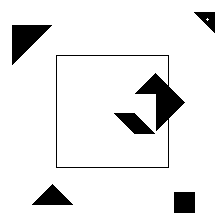
\includegraphics[width=0.2\textwidth]{images/staging_nocrop.png}}
    % \subfloat{
\includegraphics[width=0.2\textwidth]{images/staging_crop.png}}
    % \subfloat{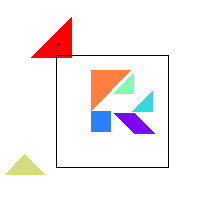
\includegraphics[width=0.2\textwidth]{images/staging_nocrop_color.png}}
    % \subfloat{
\includegraphics[width=0.2\textwidth]{images/staging_crop_color.png}}
    \subfloat{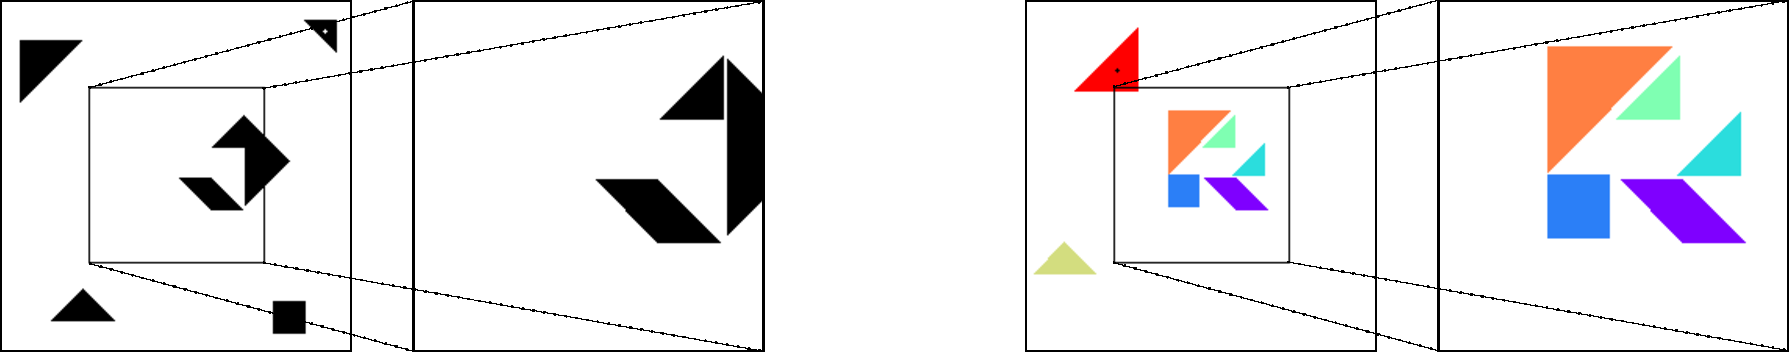
\includegraphics[width=\textwidth]{images/staging_boundaries.pdf}}
    \caption[Staging boundaries in the Tangram environment.]{Staging boundaries in the Tangram environment. Simulations using staging boundaries can be viewed at \url{https://drive.google.com/drive/folders/1PLopyNdzpWiz6CK4EvR8oEAScACpUsW0} or \url{https://t.ly/zb2cZ}.}
    \label{fig:staging-boundaries}
\end{figure}

\chapter{Controller Hyperparameters}
\label{sec:icem-details}
% task_horizon
% horizon
% num_simulated_trajectories
% cost_along_trajectory
% action_sampler_params.opt_iterations
% action_sampler_params.init_std
% action_sampler_params.elites_size
% discount_along_trajectory
The iCEM controller introduced in \secref{sec:icem} has several hyperparameters that need to be tuned for optimal performance.
\tabref{tab:icem-params} lists the hyperparameters we tweaked in our experiments, along with the best values we found.

\begin{table}[H]
    \centering
    \caption{iCEM controller parameters.}
    \begin{tabularx}{\textwidth}{C{4.7cm} L C{2cm}}
        \hline
        Property & Description & Best\\
        \hline
        \texttt{horizon} & Number of steps in the future to plan, \(\eta\) & \(16\).\\
        \texttt{n\_trajectories} & Number of trajectories to sample, \(\nu\). & \(128\)\\
        \texttt{cost\_along\_trajectory} & Cost/reward aggregation function to evaluate the trajectory, \(\mathit{\Upsilon}\). See \secref{sec:reward-aggregation} for explanations. & \texttt{best} or \texttt{sum}\\
        \texttt{n\_inner\_iterations} & Number of iterations for the inner optimization loop, \(\iota\). & \(3\)\\
        \texttt{init\_std} & Standard deviation at which the sampling distribution is initialized, \(\bmsigma_0\). & \(0.6\)\\
        \texttt{elites\_size} & Size of the elite set, \(\kappa\). See \eqref{eq:icem-filter}. & \(20\)\\
        \texttt{discount\_factor} & Discount factor for returns expected in the future, \(\gamma\). See \eqref{eq:reward-aggregation-sum-discount}. & \(1.0\)\\ 
        \hline
    \end{tabularx}
    \label{tab:icem-params}
\end{table}

The other important hyperparameters that we did not tweak in our experiments are listed in \tabref{tab:icem-params-fixed}.

% factor_decrease_num: 1
% alpha: 0.1
% relative_init: true
% keep_previous_elites: true
% shift_elites_over_time: true
% fraction_elites_reused: 0.3
% use_mean_actions: true
% noise_beta: 3.5

\begin{table}[H]
    \centering
    \caption{iCEM controller fixed parameters.}
    \begin{tabularx}{\textwidth}{C{4.7cm} L C{2cm}}
        \hline
        Property & Description & Default\\
        \hline
        \texttt{factor\_decrease\_num} & Factor by which population size is decreased, \(\delta\). & \(1.0\)\\
        \texttt{alpha} & Momentum term for updating parameters of the sampling distribution, \(\alpha\). & \(0.1\)\\
        % \texttt{relative\_init} & \\
        \texttt{keep\_previous\_elites} & A flag to enable passing elites to the next timestamp (outer iteration). & True\\
        \texttt{shift\_elites\_over\_time} & A flag to enable passing elites over inner iterations. & True\\
        \texttt{fraction\_elites\_reused} & Fraction of passed elites from the previous iteration (inner/outer) added to the sampled trajectory set, \(\zeta\). & \(0.3\)\\
        \texttt{use\_mean\_actions} & If the mean of the sampling distribution is appended to the elite set at the end of inner iterations. & True\\
        \texttt{noise\_beta} & Colored noise exponent of the distribution, \(\beta\) & \(1.0\).\\
        \hline
    \end{tabularx}
    \label{tab:icem-params-fixed}
\end{table}

Please refer to the original paper \citep{icem} for more details on the parameters of iCEM.

\chapter{Reward Hyperparameters}
\label{sec:reward-details}

This chapter details the hyperparameters of the reward functions used in our experiments.

\section{Semantics Reward}
\label{sec:semantics-reward-details}

\subsection{Semantics Entropy Reward}
\label{sec:semantics-entropy-reward-details}
% label_prefix
% label_suffix
% categories
% semantics_baseline
% semantics_image_baseline
% semantics_alpha_target
% semantics_beta_image
% semantics_model_temperature
% semantics_model_version
% semantics_normalize
% semantics_reward_scale

\tabref{tab:entropy-reward-params} lists the parameters of the regularized semantics entropy reward from \eqref{eq:entropy-reward-reg}, along with the best values we found for our experiments.
\begin{table}[H]
    \centering
    \caption{Semantics entropy reward parameters.}
    \begin{tabularx}{\textwidth}{C{3.9cm} L C{2cm}}
        \hline
        Property & Description & Best\\
        \hline
        \texttt{categories} & List of creative possibilities, \(\bmc\). & \(|c| \approx 20\)\\
        \texttt{label\_prefix} & Prefix to be added to the categories to create text labels.\\
        \texttt{label\_suffix} & Suffix to be added to the categories to create text labels.\\
        \texttt{baseline} & Baseline text input, \(\bfl_b\). ``A white canvas''\\
        \texttt{image\_baseline} & Baseline image input, \(\bfi_b\).\\
        \texttt{alpha\_text} & Regularization parameter for text inputs, \(\alpha_{l}\). & \(0.5\)\footnotemark[1]\\
        \texttt{beta\_image} & Regularization parameter for input image observation, \(\beta_{i}\). & \(0\)\footnotemark[1]\\
        \texttt{model\_version} & Name of the CLIP variant used. & (\texttt{ViT-L/14})\\
        \texttt{model\_temperature} & Temperature for the softmax function in the semantics entropy reward, \(\tau\). & \([1, 2]\)\\
        \texttt{normalize} & If the reward should be normalized by maximum entropy, \(\log(|\bmc|)\). & True\\
        \texttt{reward\_scale} & Factor with which the reward is scaled. Together with the \texttt{reward\_scale} for the regularity reward, this determines the reward ratio, \(\lambda\) from \eqref{eq:semantics-reward}. & \(1.0\)\\
        \hline
    \end{tabularx}
    \label{tab:entropy-reward-params}
\end{table}

The list of creative possibilities we typically used in Tangram is -- ``house'', ``bird'',``tree'',``horse'', ``rabbit'', ``goat'', ``shirt'', ``chair'', ``swan'', ``goose'', ``camel'', ``teapot'', ``hammer'', ``boot'', ``key'', ``gun'', ``apple'', ``car'', ``guitar'', ``flower'', and ``heart''.
Since some categories were identified to be preferred by CLIP, such as ``house'' and ``bird'', they were removed in some experiments.

In ShapeGridWorld, we typically used either a set of all single-digit numbers or numbers with letters together.
We also experimented with the above list of categories in ShapeGridWorld.
The effects of this choice are also compared in \secref{sec:sgw-categories}.

\footnotetext[1]{Please see \secref{sec:alpha-beta-semantics} for more details.}

\newpage
\subsection{Regularity Reward}
\label{sec:regularity-reward-details}
% compression_precision
% compression_granularity
% compression_bidirectional
% compression_normalize
% compression_reward_scale

In the introduction to the regularity reward in \secref{sec:regularity-reward}, we mentioned the additional hyperparameters \(\omega\) -- \emph{resolution} and \emph{bidirectionality}.
This section provides more details about these hyperparameters.

The hyperparameter for resolution consists of two parts -- precision and granularity.
The following equation extends \eqref{eq:rair-relational} with these hyperparameters to define the \(\lfloor \cdot \rceil\) operator.
\begin{equation}
    \lfloor s^{(j)} - s^{(k)} \rceil = \begin{cases}\begin{aligned}
        \left\lfloor \left| s^{(j)} - s^{(k)} \right| \frac{\text{precision}}{\text{granularity}} \right\rfloor \times \text{granularity},\quad&\text{if bidirectionality} = \text{False}\\
        \left\lfloor \left( s^{(j)} - s^{(k)} \right) \frac{\text{precision}}{\text{granularity}} \right\rfloor \times \text{granularity},\quad&\text{if bidirectionality} = \text{True}\\
    \end{aligned}\end{cases}
    \label{eq:rair-relational-extended}
\end{equation}
\tabref{tab:regularity-reward-params} lists the parameters of the regularity reward, along with the (default or) best values we found for our experiments.
\begin{table}[H]
    \centering
    \caption{Regularity reward parameters.}
    \begin{tabularx}{\textwidth}{C{3.9cm} L C{2.1cm}}
        \hline
        Property & Description & Best\\
        \hline
        \texttt{precision} & Precision of the compression algorithm. & SGW - \(1\) Tangram - \(28\)\\
        \texttt{granularity} & Granularity of the compression algorithm. & \(1\)\\
        \texttt{bidirectional} & If the compression should be bidirectional. & False\\
        \texttt{normalize} & If the reward should be normalized by the maximum possible entropy, \(\log\left(\binom{N}{2}\right)\). & True\\
        \texttt{reward\_scale} & Factor with which the reward is scaled. Together with the \texttt{reward\_scale} for the semantics entropy reward, this determines the reward ratio, \(\lambda\) from \eqref{eq:semantics-reward}. & \(1.0\)\\
        \hline
    \end{tabularx}
    \label{tab:regularity-reward-params}
\end{table}

Please refer to the original paper \citep{rair} for more details on the theory and implementation of \emph{RaIR}.

\section{Closeness Reward}
\label{sec:closeness-reward-details}
% closeness_reward_type
% closeness_reward_scale
% closeness_reward_threshold

\tabref{tab:closeness-reward-params} lists the typical parameters of the closeness reward introduced in \secref{sec:closeness-rollouts}.
\begin{table}[H]
    \centering
    \caption{Closeness reward parameters.}
    \begin{tabularx}{\textwidth}{C{3.9cm} L C{2.1cm}}
        \hline
        Property & Description & Default\\
        \hline
        \texttt{reward\_type} & Type of closeness reward -- \emph{sparse-incremental} or \emph{dense}. & ``sparse''\\
        \texttt{reward\_scale} & Factor with which the reward is scaled. & \(1.0\)\\
        \texttt{reward\_threshold} & Threshold, \(\varepsilon\), for sparse rewards \eqref{eq:closeness-reward-sparse}. & \(0.051\)\\
        \hline
    \end{tabularx}
    \label{tab:closeness-reward-params}
\end{table}

% - controller_params.compression                           True
% - controller_params.render_kwargs.invert                  True
% - controller_params.render_kwargs.color                   False
% - controller_params.semantics_baseline                    "A white canvas"
% - controller_params.action_sampler_params.opt_iterations  3
% - controller_params.action_sampler_params.init_std        0.6
% - controller_params.action_sampler_params.elites_size     20
% - controller_params.num_simulated_trajectories            256
% - controller_params.horizon                               8
% - env_params.x_size                                       28
% - env_params.x_step                                       7
% - controller_params.compression_precision                 28
% - env_params.staging_boundaries                           `[[0.25, 0.25], [0.75, 0.75]]`
% - env_params.object_persistency                           0
% - controller_params.semantics_model_temperature           1
% - controller_params.semantics_alpha_target                0.5
% - controller_params.semantics_beta_image                  0
% - controller_params.semantics_reward_scale                1
% - controller_params.cost_along_trajectory                 "best"

\chapter{Comparing CLIP Models}
\label{sec:clip-comparison}

The vision transformer (ViT) models have better accuracy than Resnet models.
Resnet models have a gradual slope in rollouts compared to ViT models and flatter distributions on random images.

\begin{figure}[H]
    \centering
    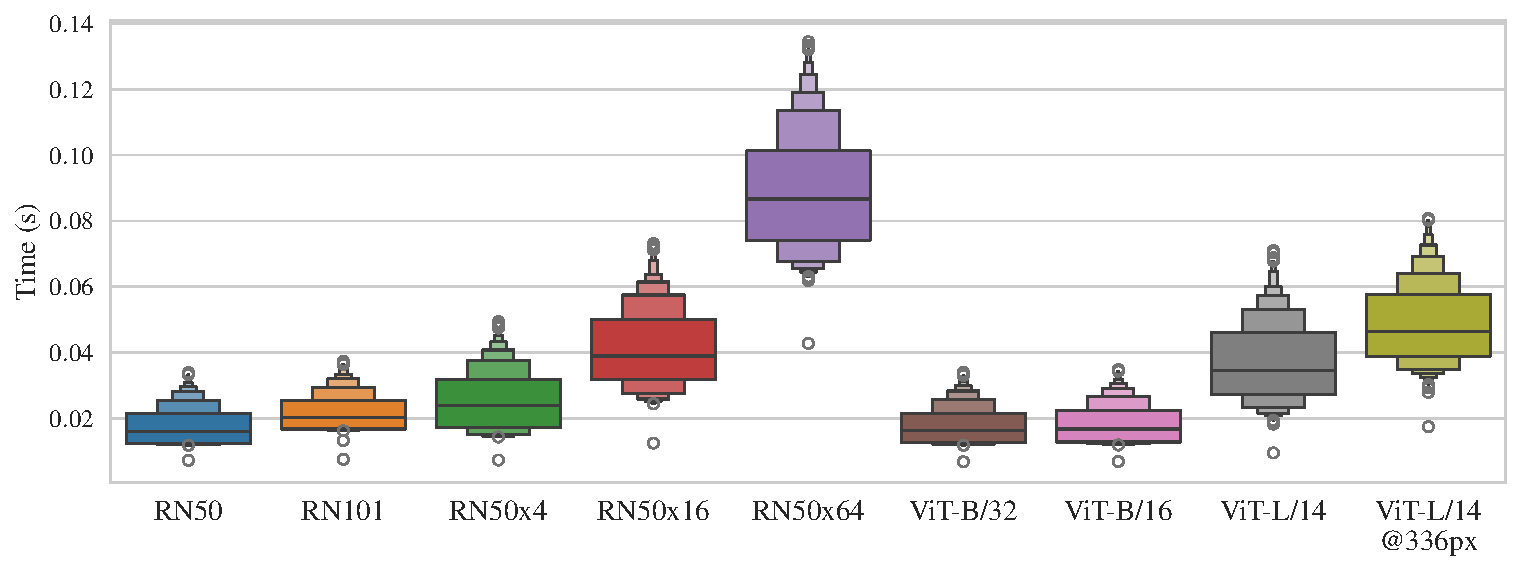
\includegraphics[width=\textwidth]{images/clip_inference_times.pdf}
    \vspace{-12pt}
    \caption{Comparing times of different original CLIP models for embedding a single image.}
    \label{fig:clip-time-comparison}
\end{figure}

\figref{fig:clip-traj-comparison-color} shows the trajectories of different CLIP models on colored Tangram environments (without RaIR).
The cumulative rewards and trajectories of the models are similar and do not give a clear picture of the models' performances, but the larger models seem to have better creations. 

% \begin{figure}[H]
%     \centering
%     % model_comparison.pdf
%     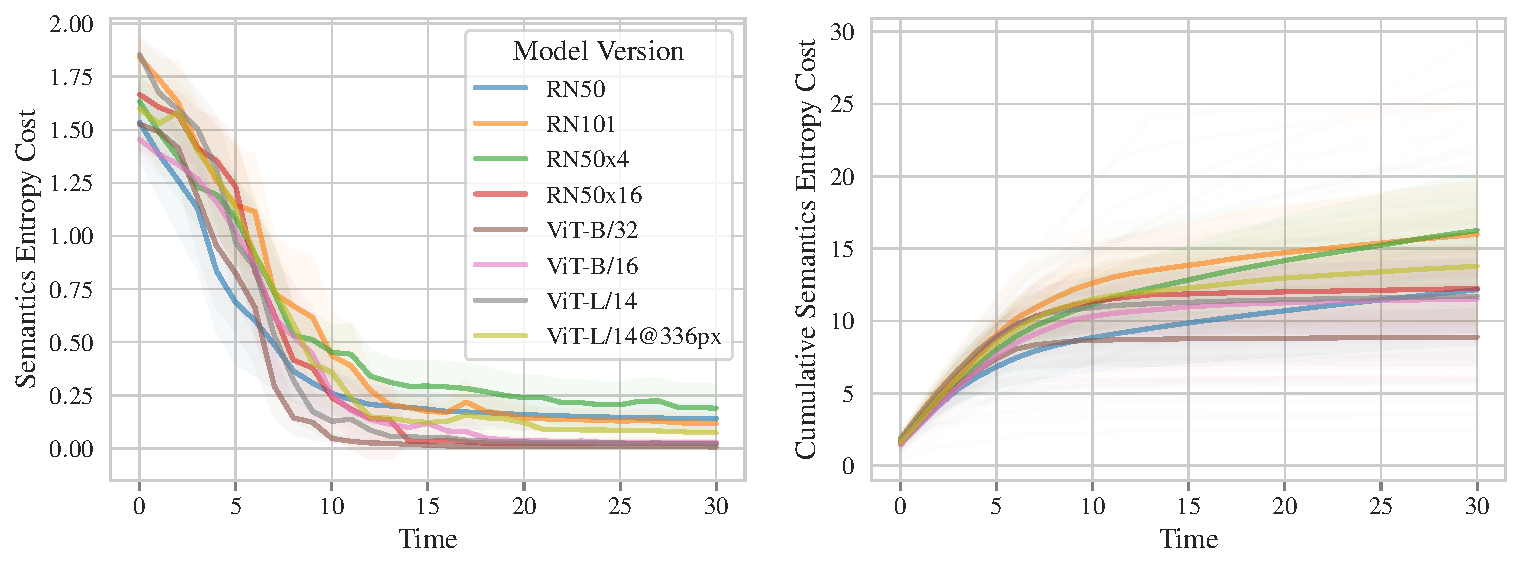
\includegraphics[width=\textwidth]{images/model_comparison.pdf}
%     % model_comparison_boxplot.pdf
%     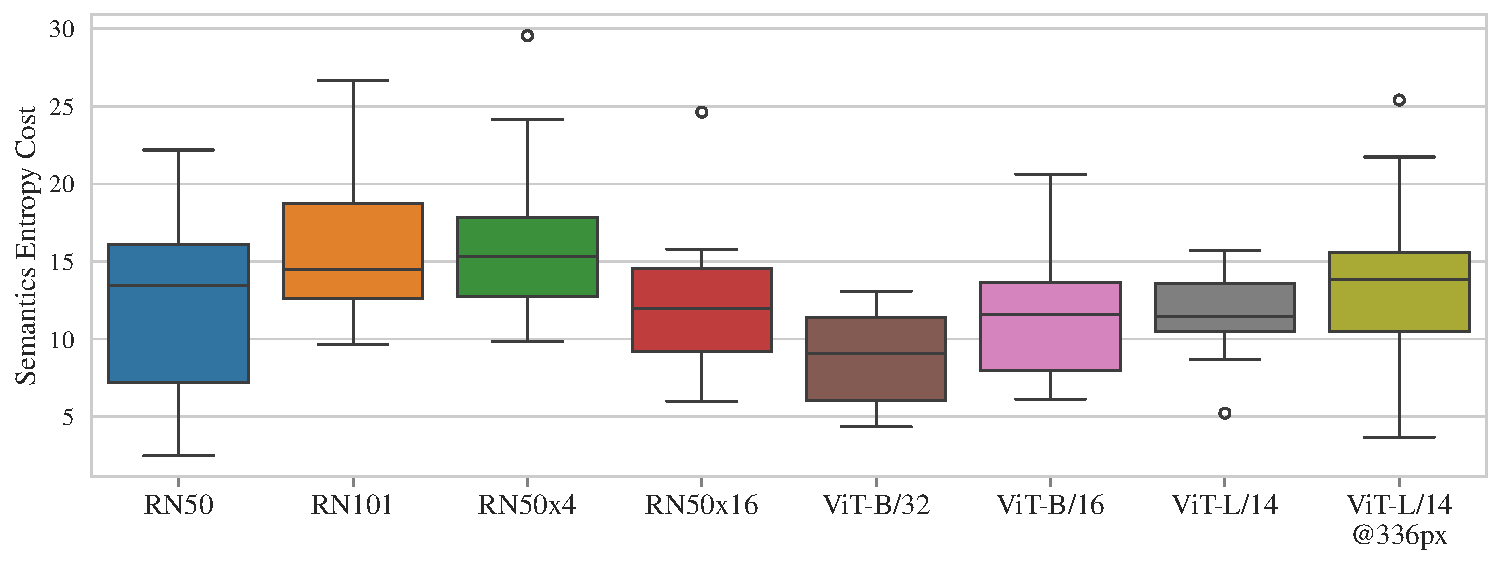
\includegraphics[width=\textwidth]{images/model_comparison_boxplot.pdf}
%     % model_samples.pdf
%     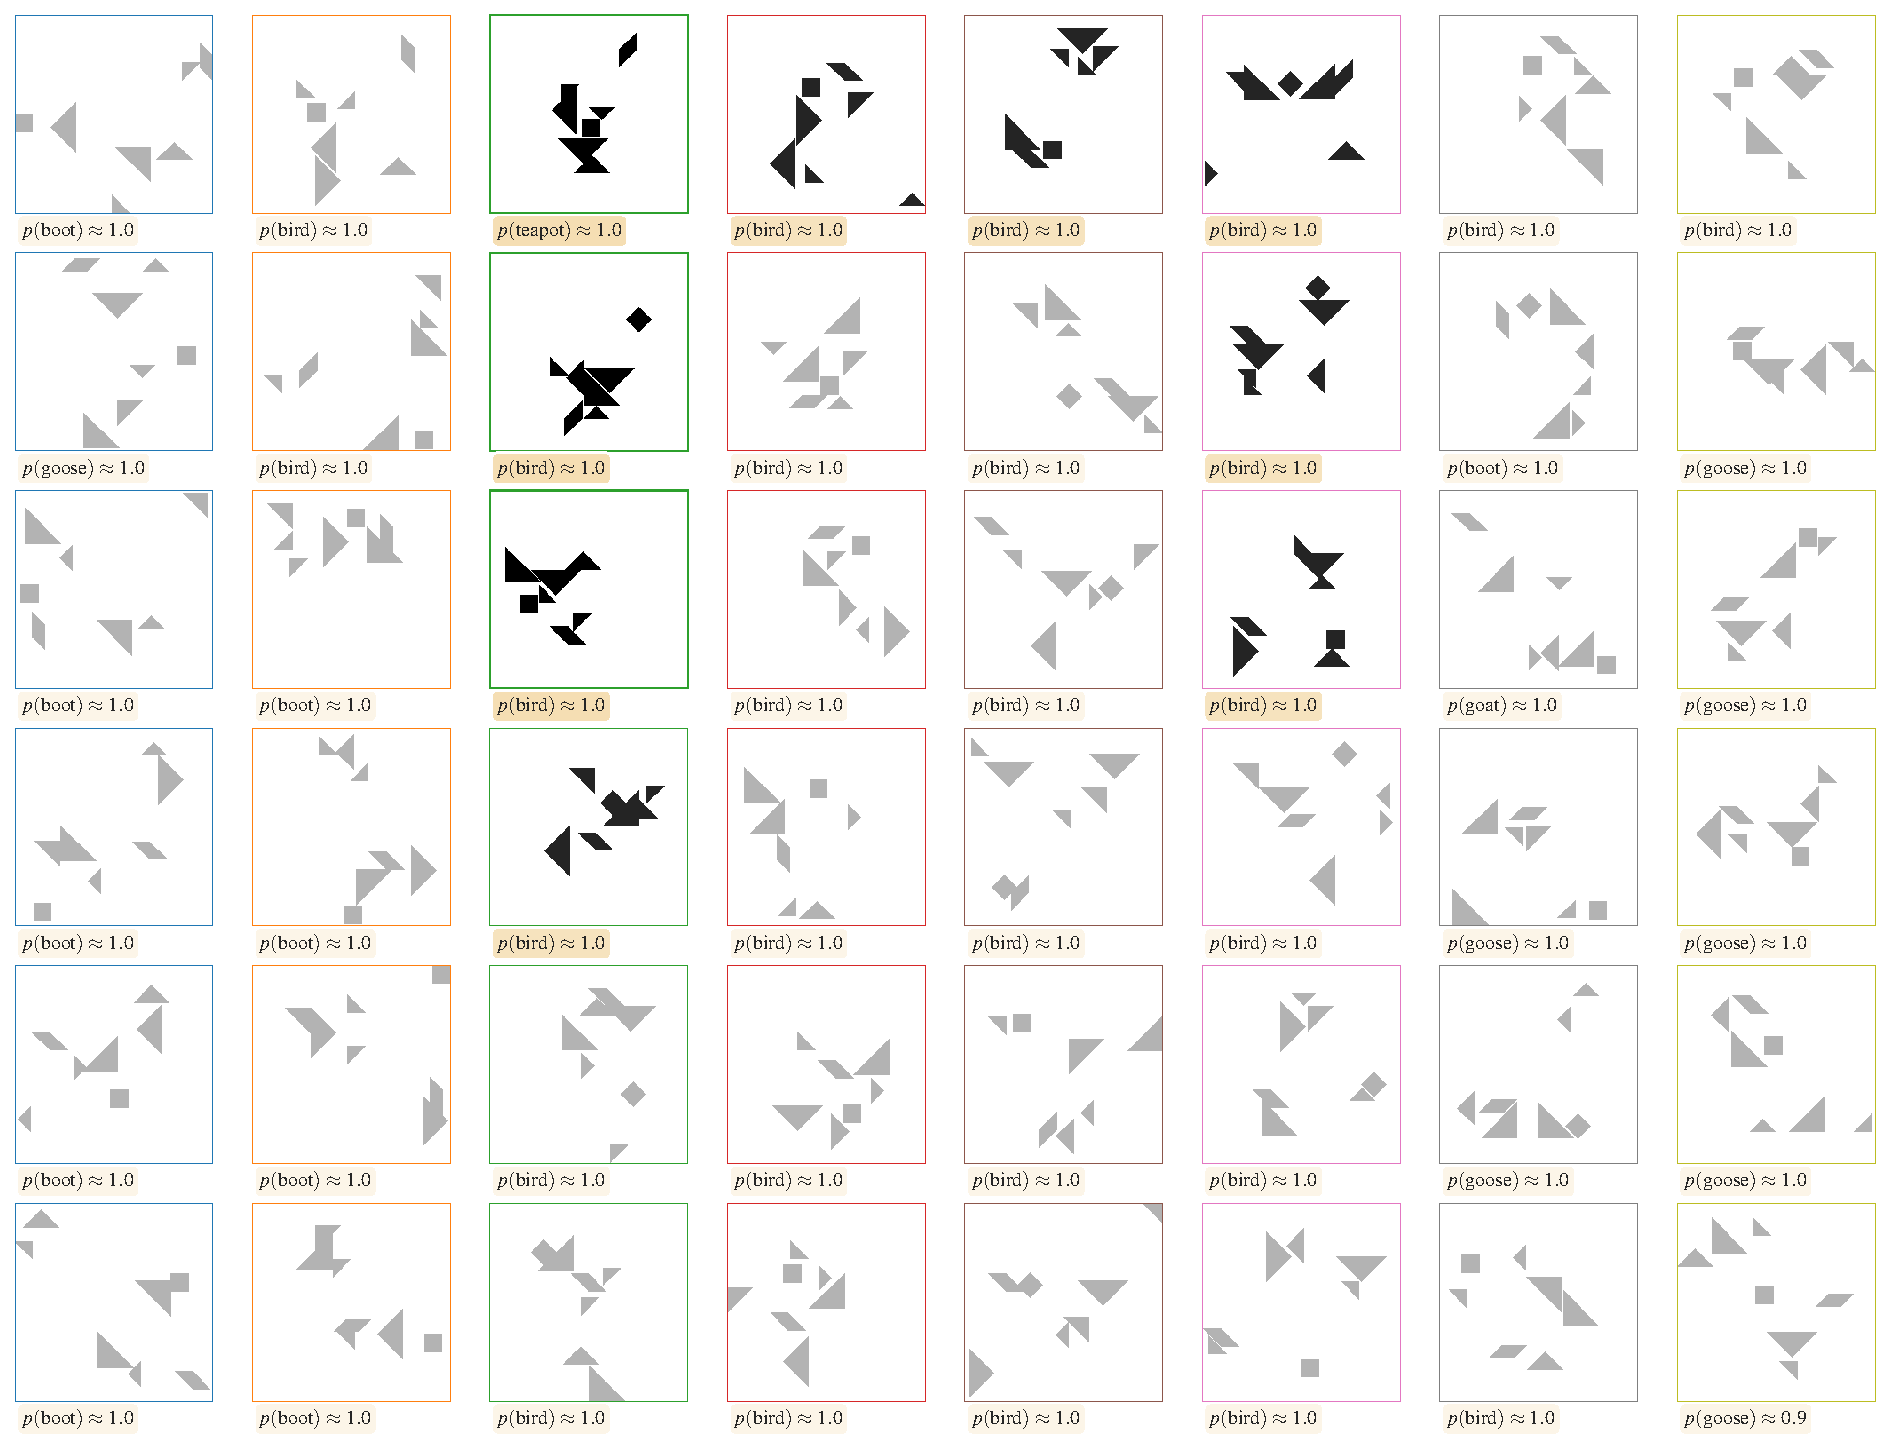
\includegraphics[width=0.9\textwidth]{images/model_samples.pdf}
%     \caption[Comparing reward trajectories of different original CLIP models on b/w Tangram environment.]{Comparing reward trajectories of different original CLIP models on b/w Tangram environment. 10 seeds were used for each model.}
%     \label{fig:clip-traj-comparison}
% \end{figure}

\begin{figure}[H]
    \centering    
    % model_comparison_color.pdf
    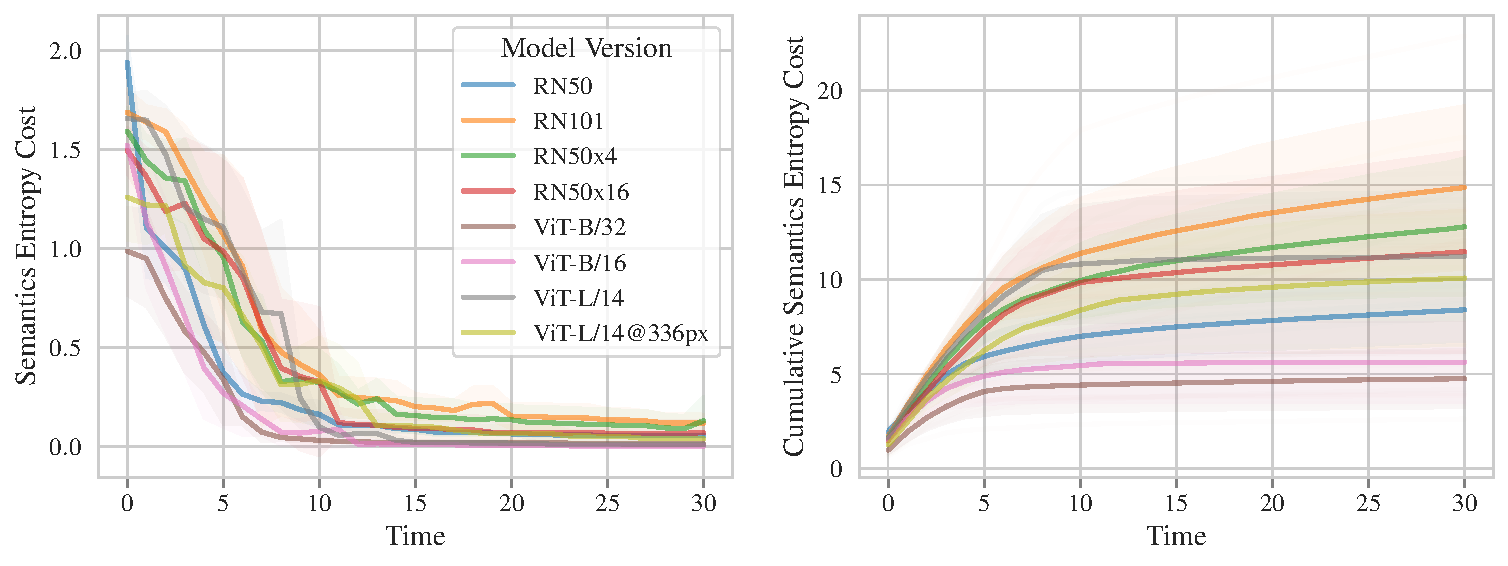
\includegraphics[width=\textwidth]{images/model_comparison_color.pdf}
    % model_comparison_boxplot_color.pdf
    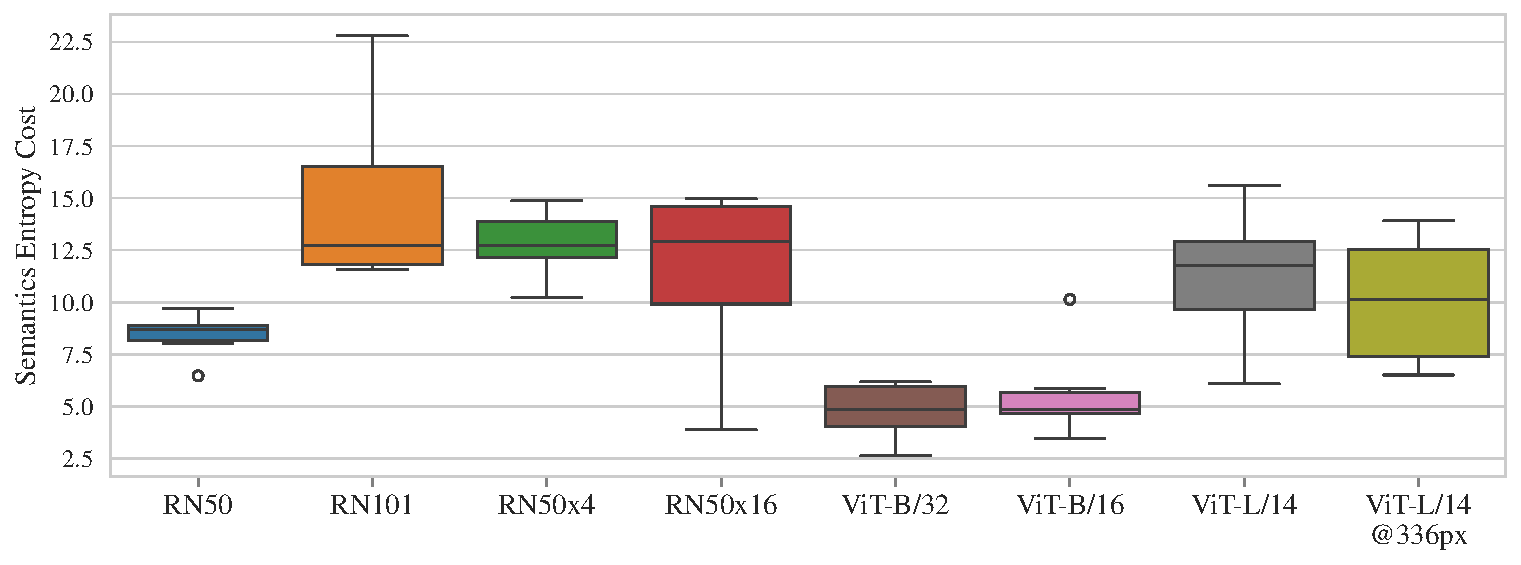
\includegraphics[width=\textwidth]{images/model_comparison_boxplot_color.pdf}
    % model_samples_color.pdf
    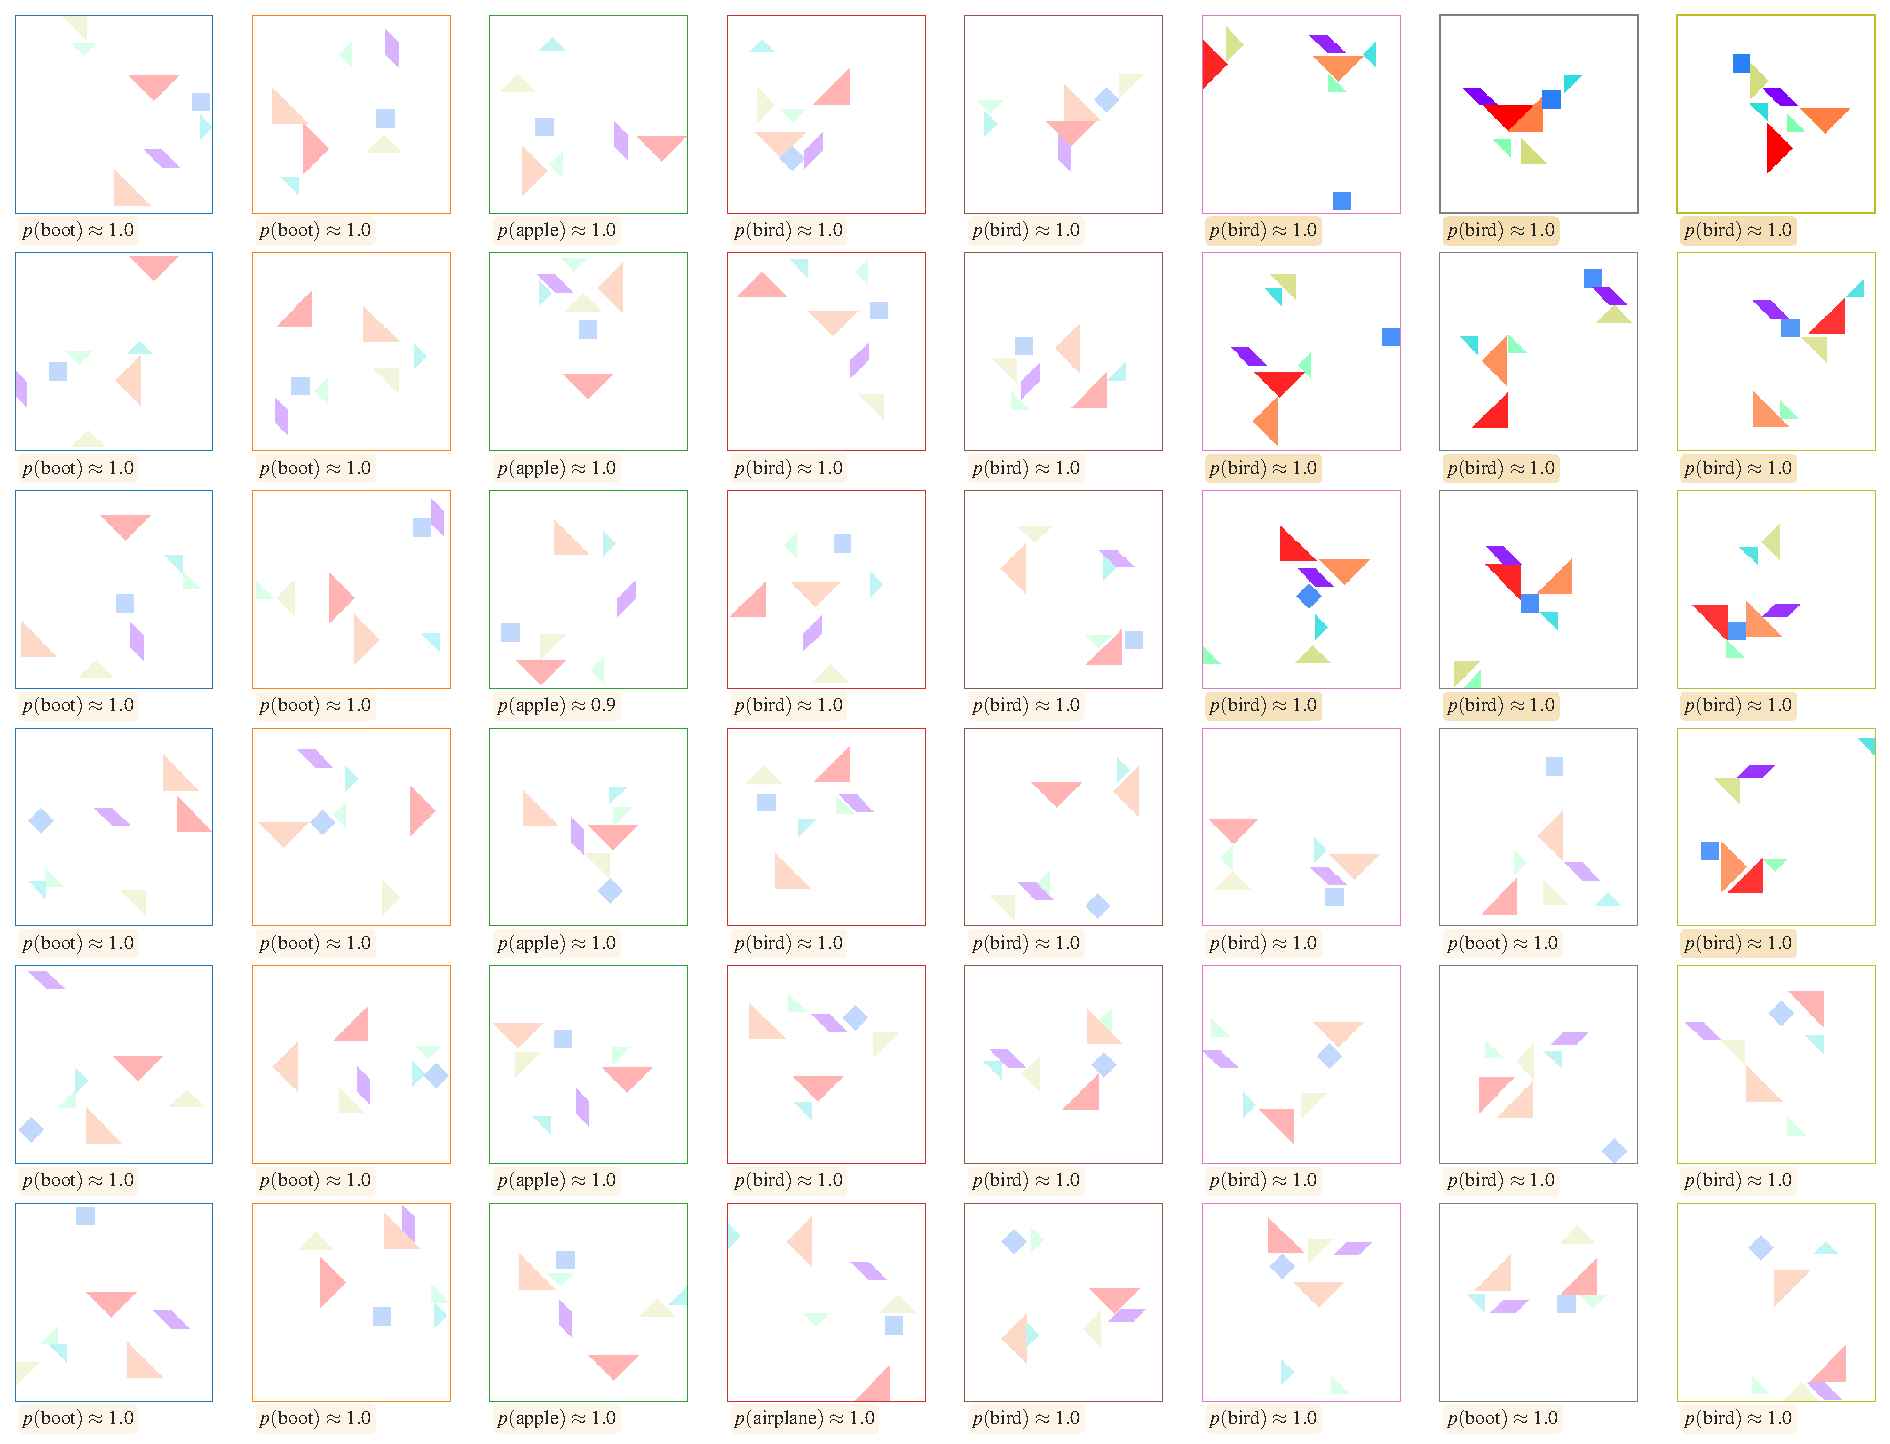
\includegraphics[width=0.9\textwidth]{images/model_samples_color.pdf}
    \caption[Comparing reward trajectories of different original CLIP models on colored Tangram environment.]{Comparing reward trajectories of different original CLIP models on colored Tangram environment. 10 seeds were used for each model.}
    \label{fig:clip-traj-comparison-color}
\end{figure}


\chapter{Flatnet}
\label{sec:flatnet}
To test the feasibility and efficacy of fine-tuning CLIP with an entropy regularization technique \eqref{eq:entropy-regularization} to reduce its inference noise, we conducted experiments on a smaller \emph{toy} setup with convolutional neural networks trained as a single-digit number classifier on ShapeGridWorld registered images from the MNIST dataset \citep{mnist}.
We additionally augment the MNIST training dataset with samples of images with random arrangements of pixels, target-labeled with a uniform distribution of confidence over the ten single digits.

We treated the entropy regularization strength and the addition of random samples as hyperparameters and trained a series of models with different combinations of the two.
% \figref{fig:flatnet-comparison} shows the resulting trajectories of the models.
The models were trained with the Adam optimizer \citep{adam} with a learning rate of \(0.001\) and a batch size of \(128\). The size of the MNIST training dataset is \(60000\).
\tabref{tab:flatnet-models} summarizes the models we compare.
More details of these models can be found at \url{https://pulkitgoyal56.github.io/flatnet}.

% \vspace{12pt}
\begin{table}[H]
    \centering
    \caption{Summary of the Flatnet models.}
    \begin{tabularx}{0.7\textwidth}{c c c c}
    \hline
        Serial & Name & Random Training Data Size & \(\lambda\) \\ \hline
        Flatnet 0 (lite) & flatnetlite & 0 & 0.0 \\ \hline
        Flatnet 1 (lite) & flatnetlite & 0 & 0.2 \\ \hline
        Flatnet 2 & flatnet & 0 & 0.2 \\ \hline
        Flatnet 3 & flatnet & 0 & 0.4 \\ \hline
        Flatnet 4 & flatnet & 0 & 0.6 \\ \hline
        Flatnet 5 & flatnet & 0 & 0.8 \\ \hline
        Flatnet 6 & flatnet & 0 & 1.0 \\ \hline
        Flatnet 7 & flatnet & 10000 & 0.0 \\ \hline
        Flatnet 8 & flatnet & 10000 & 0.3 \\ \hline
        Flatnet 9 & flatnet & 10000 & 0.7 \\ \hline
        Flatnet 10 & flatnet & 10000 & 0.8 \\ \hline
        Flatnet 11 & flatnet & 10000 & 1.0 \\ \hline
        Flatnet 12 & flatnet & 0 & 1.0 \\ \hline
        Flatnet 13 & flatnet & 60000 & 0.0 \\ \hline
        Flatnet 15 & flatnet & 0 & 0.0 \\ \hline
    \end{tabularx}
    \label{tab:flatnet-models}
\end{table}

\figref{fig:flatnet-comparison} compares the reward trajectories of a regular Flatnet model and an entropy regularized Flatnet model on random rollouts (similar to \figref{fig:random-rollout}) on a grid-registered image of the number zero.
The comparisons of all the models are neatly visualized at \url{https://www.sharecanvas.io/p/flatnet-comparison}.

\begin{figure}[H]
    \centering
    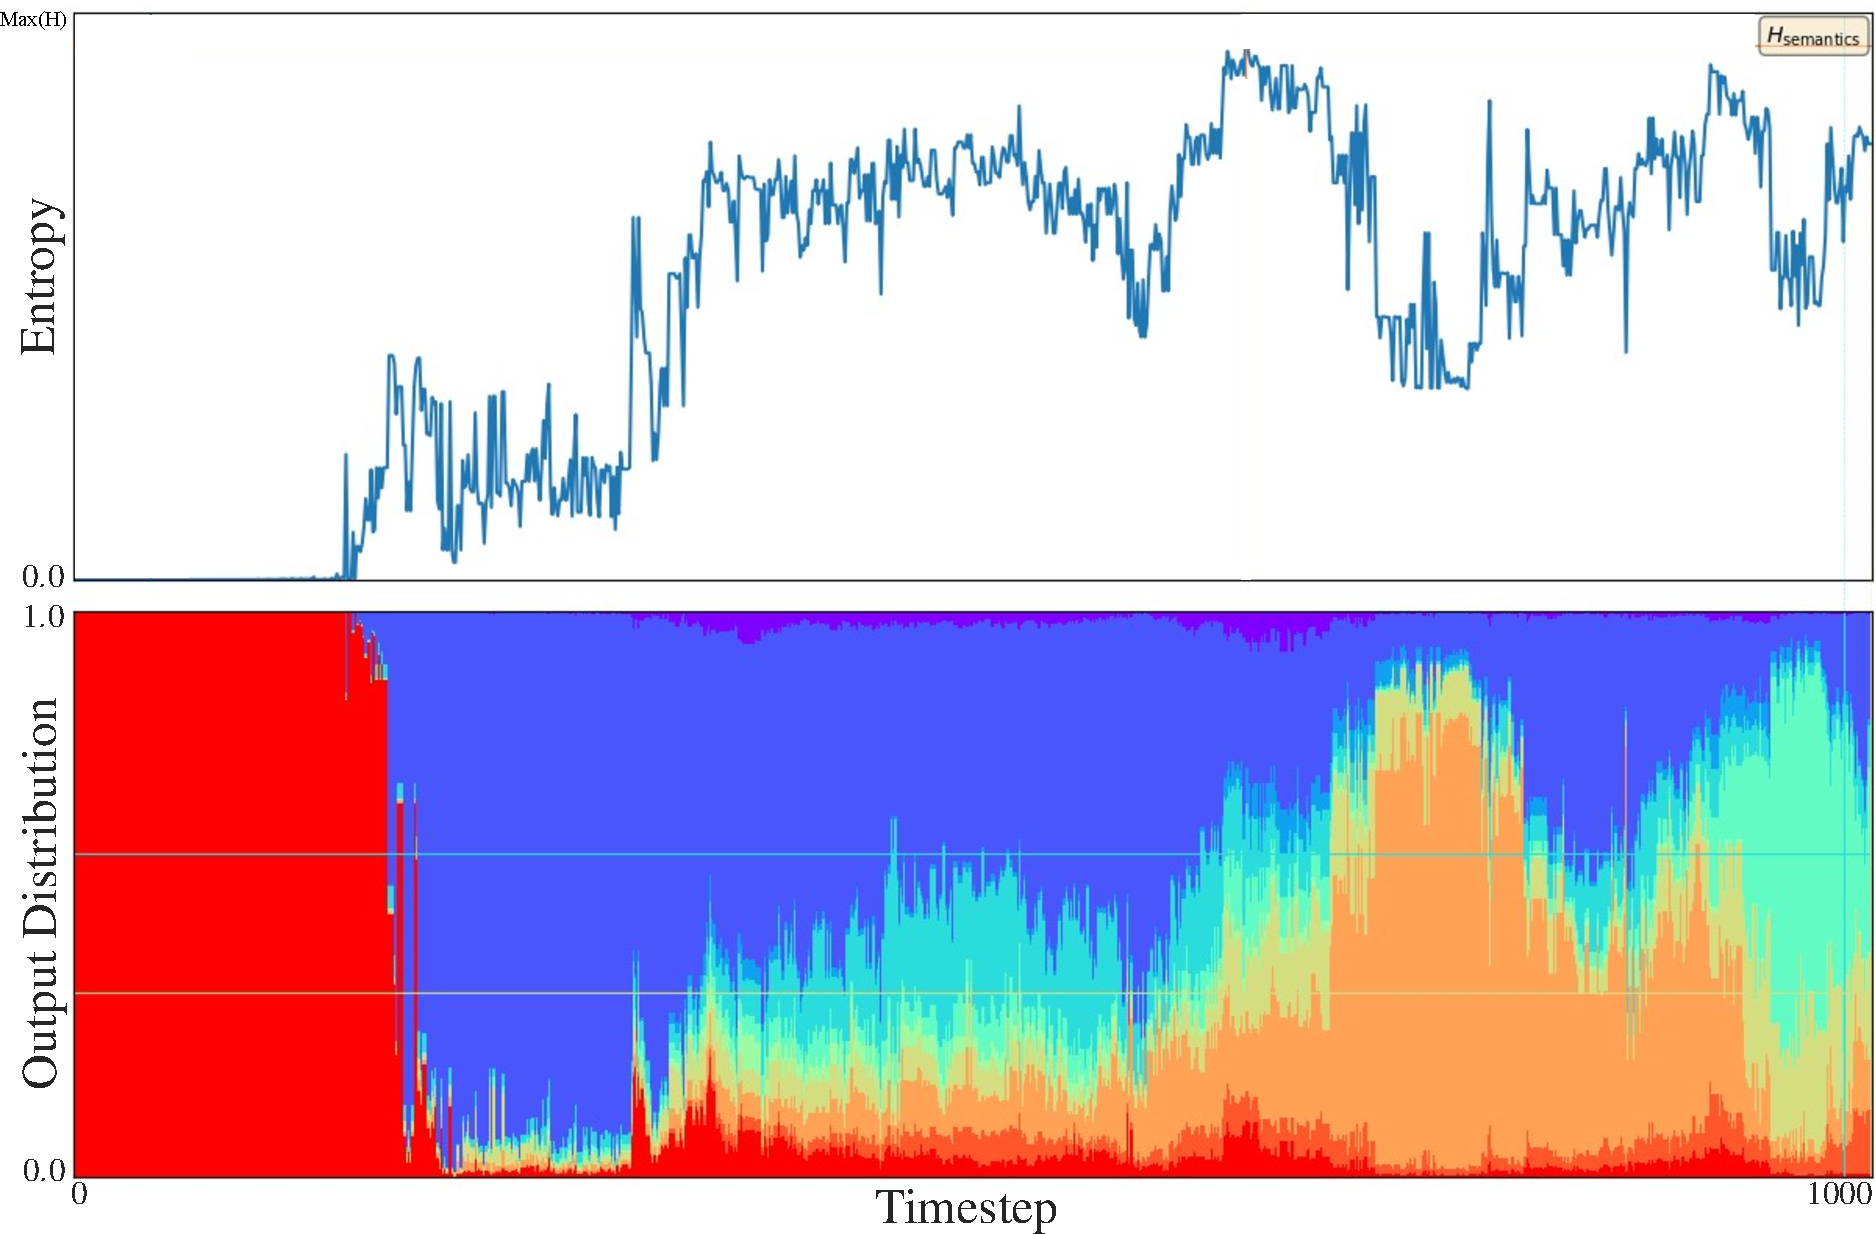
\includegraphics[width=0.8\textwidth]{images/Flatnet 15.pdf}
    \caption[A regular Flatnet MNIST classifier on random rollouts.]{A regular Flatnet MNIST classifier on random rollouts. Flatnet 15.}
    \vspace{12pt}
    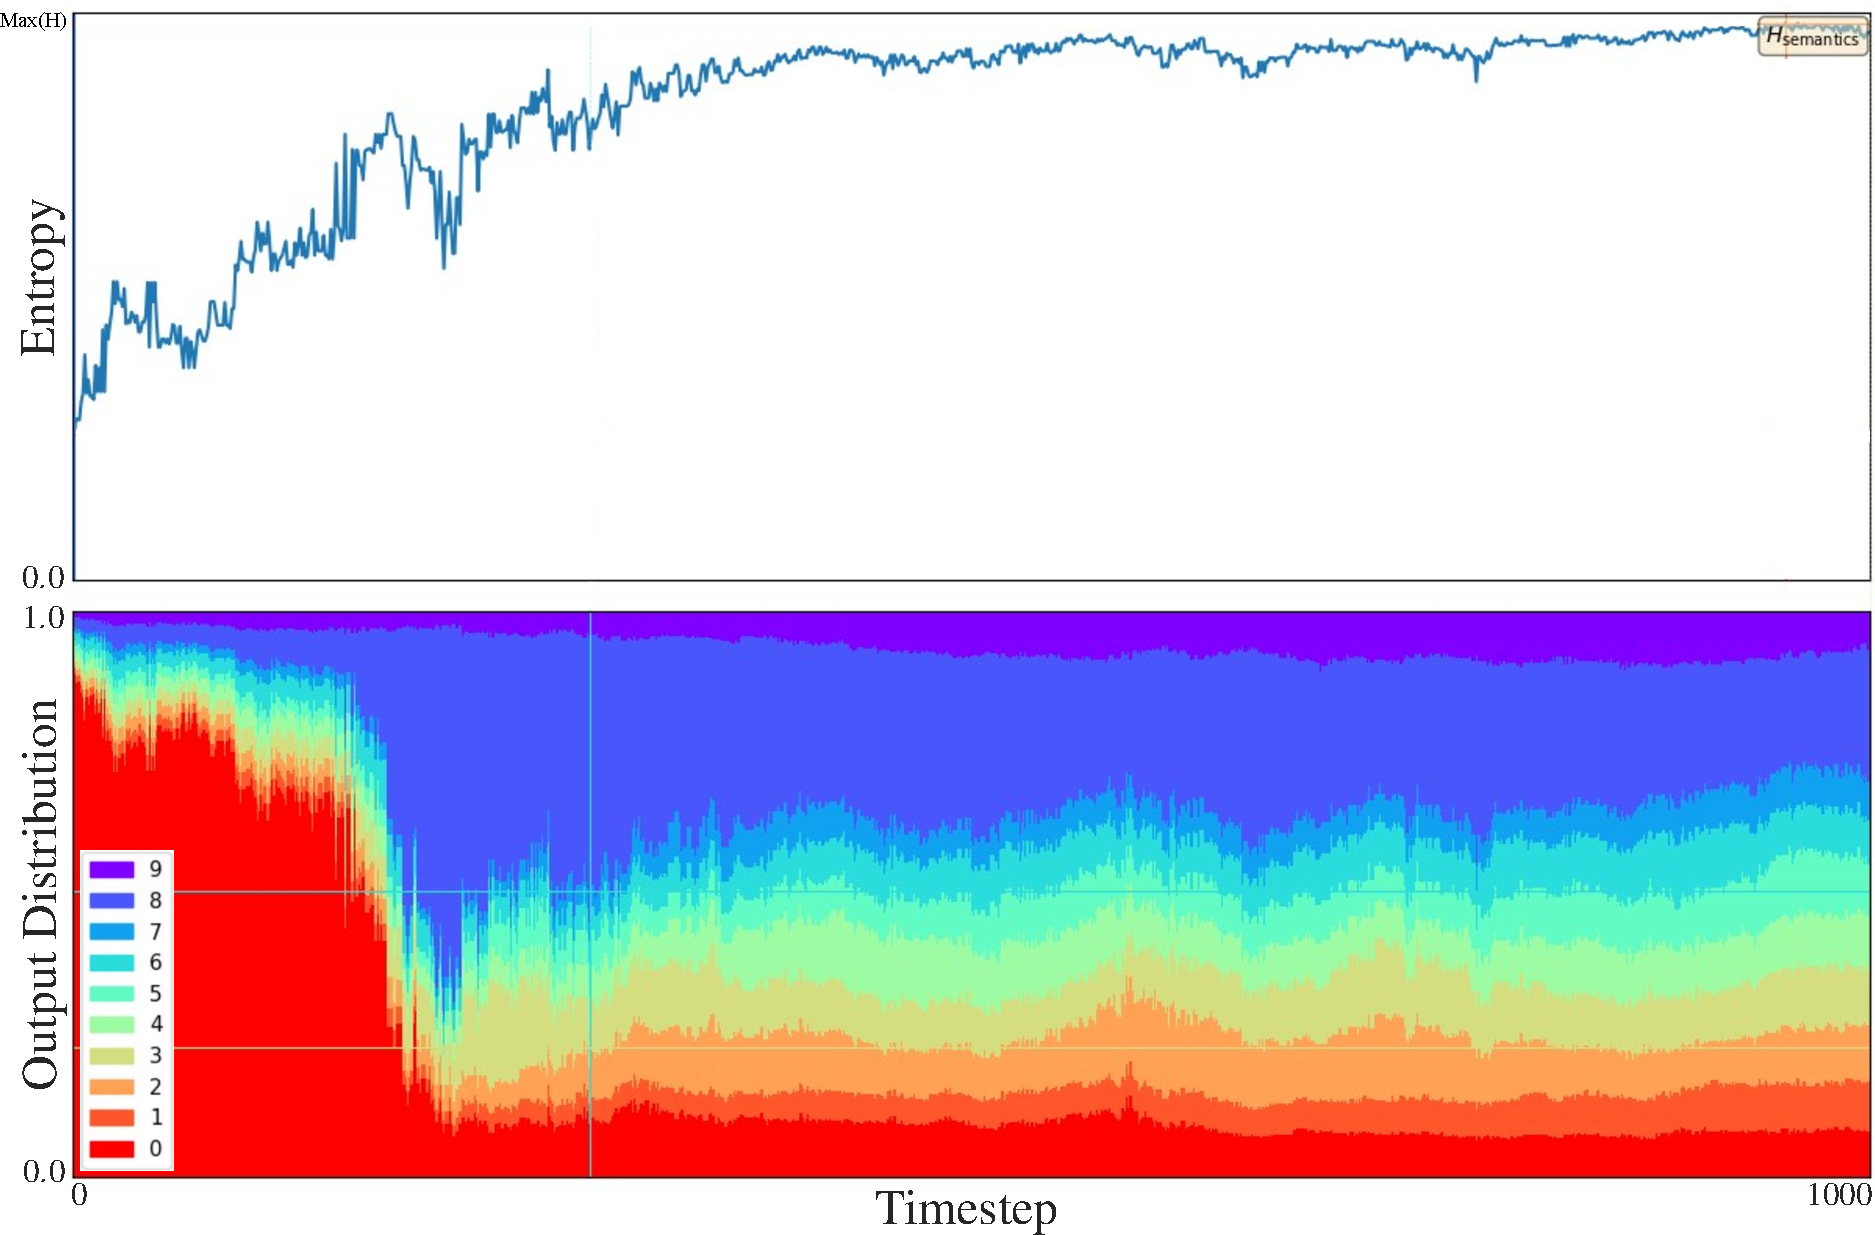
\includegraphics[width=0.8\textwidth]{images/Flatnet 3.pdf}
    \caption[An entropy regularized Flatnet MNIST classifier on random rollouts.]{An entropy regularized Flatnet MNIST classifier on random rollouts. Flatnet 3.}
    \label{fig:flatnet-comparison}
\end{figure}

Both, the entropy regularization and the addition of random samples, helped improve the reward trajectories of the models.
The regularized models have smoother entropy transitions, a stable distribution over time, and a flatter distribution (high entropy) for false positive (random) samples.


% \chapter{Descriptive List of Main Hyperparameters}
% \label{sec:hyperparameters}
% Here, we provide a list of the hyperparameters we mainly considered in our experiments.


\chapter{Improving Simulation Times}
\label{sec:efficiency}
Rendering the environment and using CLIP for planning was a very resource-intensive operation.
At every planning step, a total of \(\text{n\_trajectories} (\nu) \times \text{horizon} (\eta) \times \text{n\_icem\_inner\_iterations} (\iota)\) evaluations needed to be computed.
This was further multiplied by the number of steps in the simulation.
This total ranged anywhere from \(~200,000\) to \(~2,000,000\) in our many experiments which corresponded to about \(2\) to \(20\) hours of simulation time if run in a single batch of inference on multiple GPUs.

Thus, reducing simulation time was critical for us to be able to do any hyperparameter analysis.
We implemented several optimization techniques to improve this, which mainly involved efficient \emph{vectorization} of all computations, lazy evaluation, caching, parallelization, and cutting down on redundant operations.
In particular, two of these, for rendering and inference, are briefly introduced in the following sections.

\section{Reducing Rendering Time}
\label{sec:improving-render}
The rendering time was a major bottleneck for the simulations.
To improve this, we experimented with three popular open-source graphics Python libraries; \emph{Matplotlib} \citep{matplotlib}, \emph{Scikit-Image} \citep{skimage}, and \emph{OpenCV} \citep{opencv}, for both colored and grayscale renderings.
We used their functions in different formulations to further optimize their use.
The results of the best formulation for each of these libraries are summarized in \tabref{tab:render-time-color} and \tabref{tab:render-time-bw}.\\

\begin{table}[H]
    \centering
    \caption{Colored rendering-time comparison.}
    \begin{tabular}[t]{@{} c c c @{}}
        \hline
        \textbf{Library} & \textbf{Main Function/Class} & \textbf{Time (\(\mu s\))*}\\
        \hline
        Matplotlib & \texttt{PatchCollection} & 14400 ± 153\\
        Scikit-Image & \texttt{draw.polygon} & 978 ± 10.8\\
        OpenCV & \texttt{fillPoly} & 66.3 ± 0.85\\
        \hline
    \end{tabular}
    \label{tab:render-time-color}
\end{table}
\begin{table}[H]
    \centering
    \caption{Grayscale rendering-time comparison.}
    \begin{tabular}[t]{@{} c c c @{}}
        \hline
        \textbf{Library} & \textbf{Main Function/Class} & \textbf{Time (\(\mu s\))*}\\
        \hline
        Matplotlib & \texttt{PatchCollection} & 14200 ± 156\\
        Scikit-Image & \texttt{draw.polygon} & 978 ± 10.8\\
        OpenCV & \texttt{fillConvexPoly} & 52.2 ± 1.04\\
        \hline
    \end{tabular}
    \label{tab:render-time-bw}
\end{table}
* - Mean \(\pm\) standard deviation of \(7\) runs; \(1,000 - 10,000\) loops each.

These results refer to the Tangram environment, but the trend was the same with ShapeGridWorld.
The complete analysis is available on \url{https://github.com/pulkitgoyal56/master-thesis-notebooks/blob/main/archive/testbed_rendering.ignore.ipynb}.

\section{Reducing Inference Time}
\label{sec:improving-infer}
To minimize the inference times with CLIP, all inferences were done in one large batch.
This required significant memory, for which we parallelized them on multiple GPUs using Pytorch \texttt{DataParallel} \citep{pytorch}.

To reduce the inference time, we tweaked the image preprocessing functions of CLIP to be adaptive to the input to ensure that no redundant operations were performed.

Additionally, we picked the rendering configurations for the environments such that the resulting renders required minimal preprocessing in the form of resizing, cropping, type conversions, or copying, which was computationally expensive.
For example, all renderings concurred with the required input for the used CLIP model (eg. \(224 \times 224\) for the \texttt{ViT-L/14} variant) used for inference to avoid any resizing.
This also helped to improve the simulation times significantly.\\

\begin{figure}[H]
    \centering
    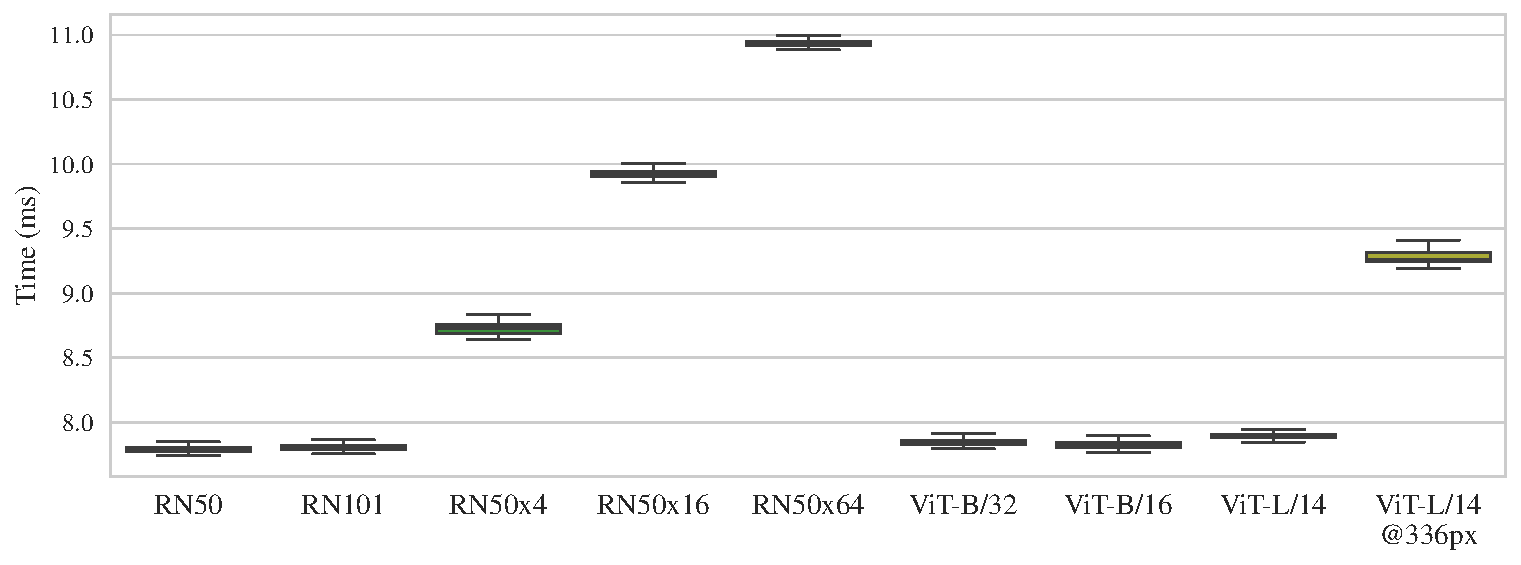
\includegraphics[width=\textwidth]{images/full_transform.pdf}
    \vspace{-12pt}
    \caption{Preprocessing times before optimizations.}
    \vspace{12pt}
    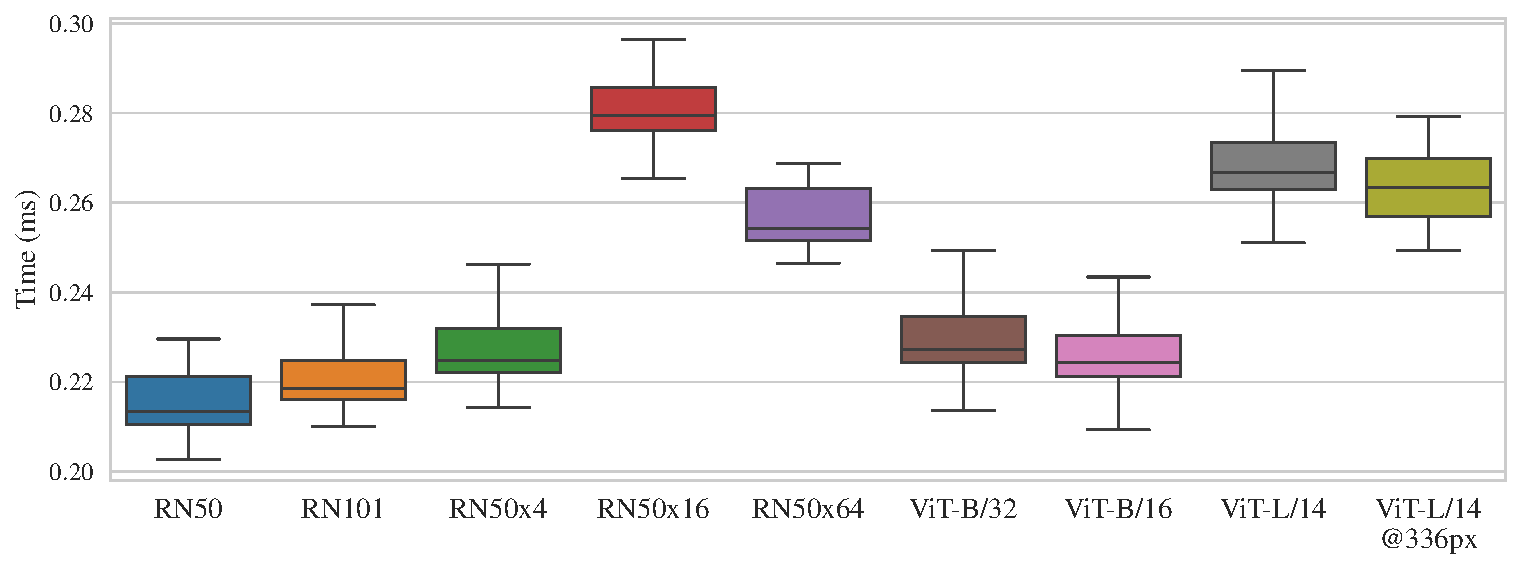
\includegraphics[width=\textwidth]{images/fast_transform.pdf}
    \vspace{-12pt}
    \caption{Preprocessing times after optimizations.}
    \label{fig:preprocessing-time-improvement}
\end{figure}

These modifications are available on \url{https://github.com/pulkitgoyal56/CLIP/tree/preprocess-tweaks}.



\chapter{More Simulations on ShapeGridWorld}
\label{sec:sgw-semantics-additional}

\section{Effect of Semantic Categories Set}
\label{sec:sgw-categories}
The effect of the choice of categories on the semantics entropy reward in ShapeGridWorld was also significant.
\figref{fig:categories-sgw} and \figref{fig:categories-sgw-norair} show the effect of different sets of categories on the reward landscape and some samples of their creations, with and without RaIR respectively.

We observe that categories involving numbers (``numbers and letters'' and ``numbers'') start with a flatter distribution compared to object categories (few\footnotemark[1] or many\footnotemark[2]).
However, we do not notice a substantial difference in the diversity of final creations due to this even starting ground.

\footnotetext[1]{The categories referred to in ``many categories'' are ``house'', ``bird'',``tree'',``horse'', ``rabbit'', ``goat'', ``shirt'', ``chair'', ``swan'', ``camel'', ``teapot'', ``hammer'', ``boot'', ``key'', ``gun'', ``apple'', ``car'', ``guitar'', ``flower'', and ``heart''.}
\footnotetext[2]{The categories referred to in ``few categories'' is the subset ``bird'', ``goat'', ``shirt'', ``swan'', ``goose'', ``teapot'', ``gun'', ``apple'', ``car'', ``airplane'', ``guitar'', and ``flower''.}

% categories_boxplot_sgw_rair.pdf
% categories_comparison_sgw_rair.pdf
% categories_samples_sgw_rair.pdf

% categories_boxplot_sgw_norair.pdf
% categories_comparison_sgw_norair.pdf
% categories_samples_sgw_norair.pdf

\section{Effect of Grayscale Pixels}
\label{sec:sgw-grayscale}
% mode_comparison_sgw.pdf
% mode_samples_sgw.pdf

% and only affected when the pixels had grayscale values
% % rair_comparison_sgw_color.pdf
% \begin{figure}[h]
%     \centering
%     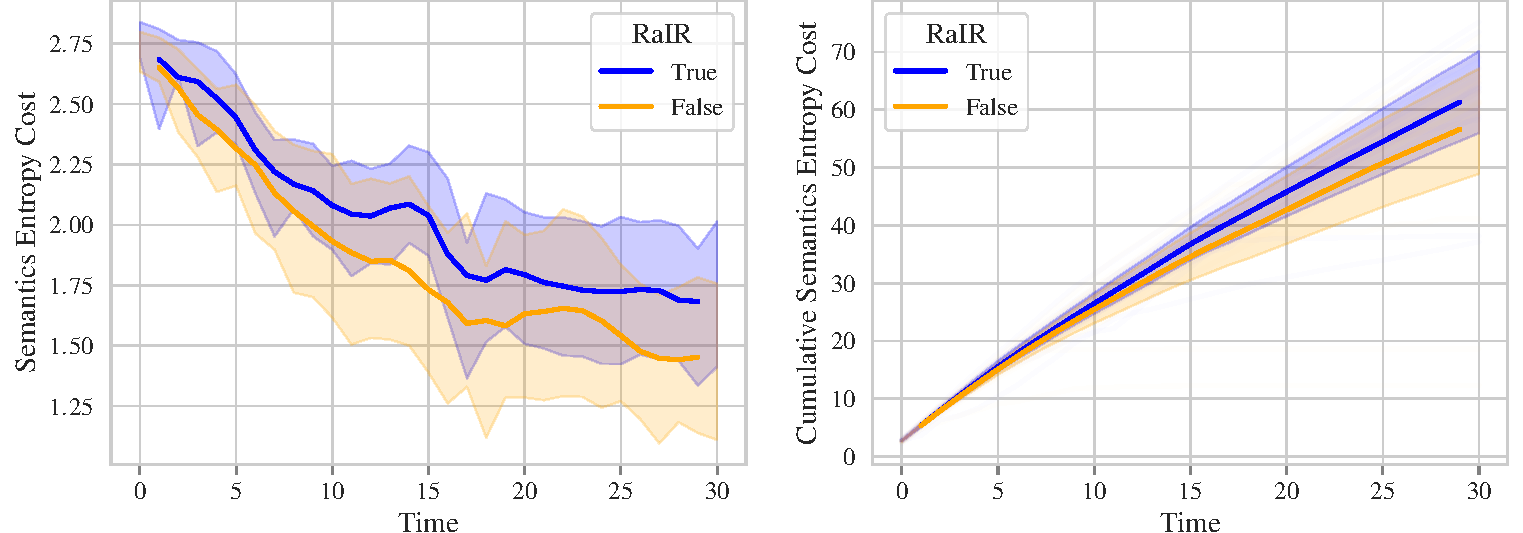
\includegraphics[width=\textwidth]{images/rair_comparison_sgw_color_cropped.pdf}
%     \caption{Effect of RaIR on ShapeGridWorld with grayscale pixels.}
%     \label{fig:rair-color-sgw}
%     \vspace{12pt}
%     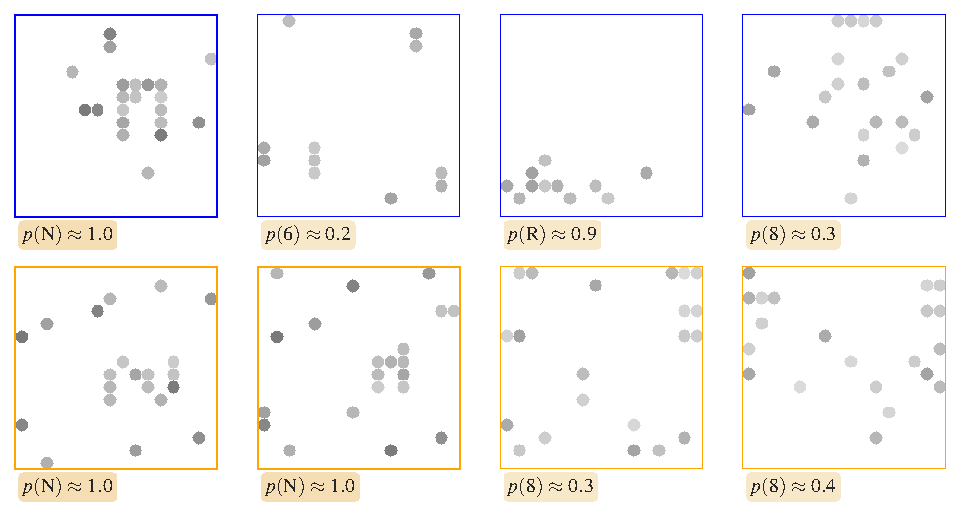
\includegraphics[width=0.5\textwidth]{images/rair_samples_sgw_color.pdf}
%     \caption{Samples of creations with and without RaIR in ShapeGridWorld with grayscale pixels.}
%     \label{fig:rair-samples-color-sgw}
% \end{figure}

Observing the effect of the grayscale values on the effect of RaIR in ShapeGridWorld, we also ran simulations with different categories of colors in the pixels.

It seems that the presence of grayscale pixels has a regularizing effect on the reward landscape and consequently there is less noise in CLIP.
This is evident from the reduced confidence in the imperfect final creations in \figref{fig:mode-sgw}.

\section{Effect of Number of Pixels}
\label{sec:sgw-pixels}
% Threshold Ratio
% n_objects_comparison_sgw.pdf
% n_objects_samples_sgw.pdf

As we noted earlier, the presence of a high number of controllable pixels in the ShapeGridWorld exacerbates the problem of noise in CLIP and is also a more difficult control problem, hence we also experimented with different numbers of pixels in the environment.

Having too few pixels also results in a rather noisy landscape with a lot of false positives, as seen in \figref{fig:n-objects-sgw}.
This seems to suggest that moderate numbers of pixels are optimal for the environment.

The effects of the number of objects, grayscale pixels, and RaIR are summarised in \figref{fig:nobj-mode-sgw}.

\begin{figure}[H]
    \centering
    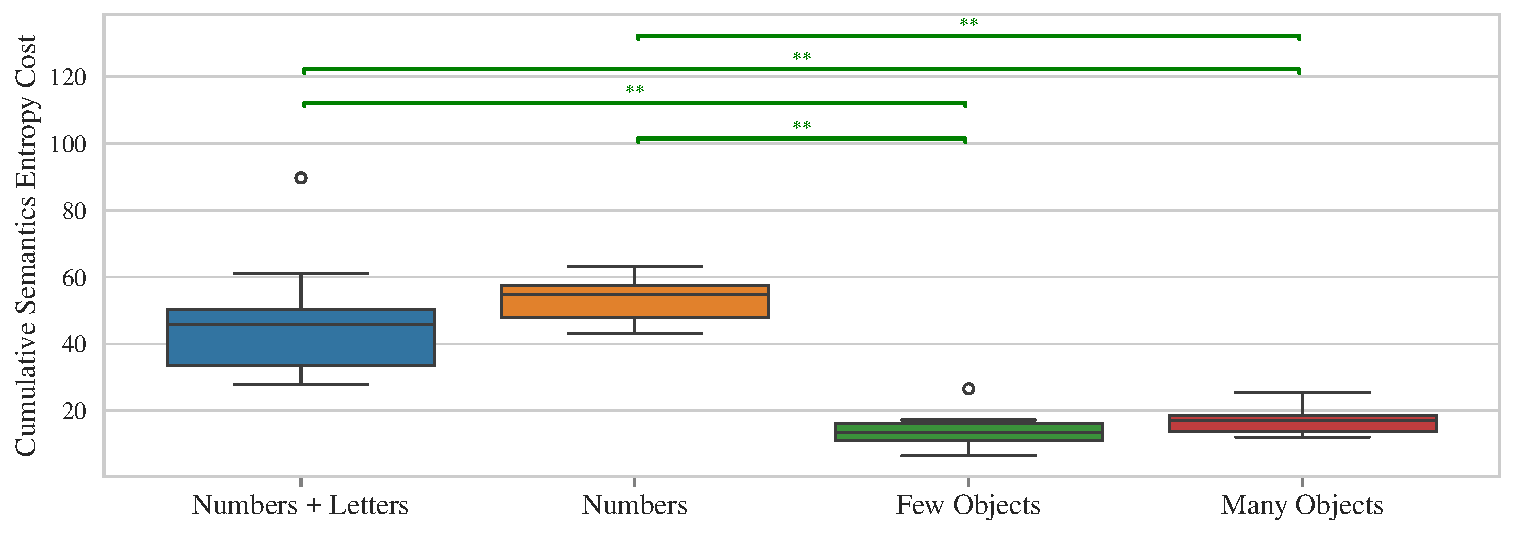
\includegraphics[width=\textwidth]{images/categories_boxplot_sgw_rair_cropped.pdf}\vspace{6pt}
    % \label{fig:categories-boxplot-sgw}
    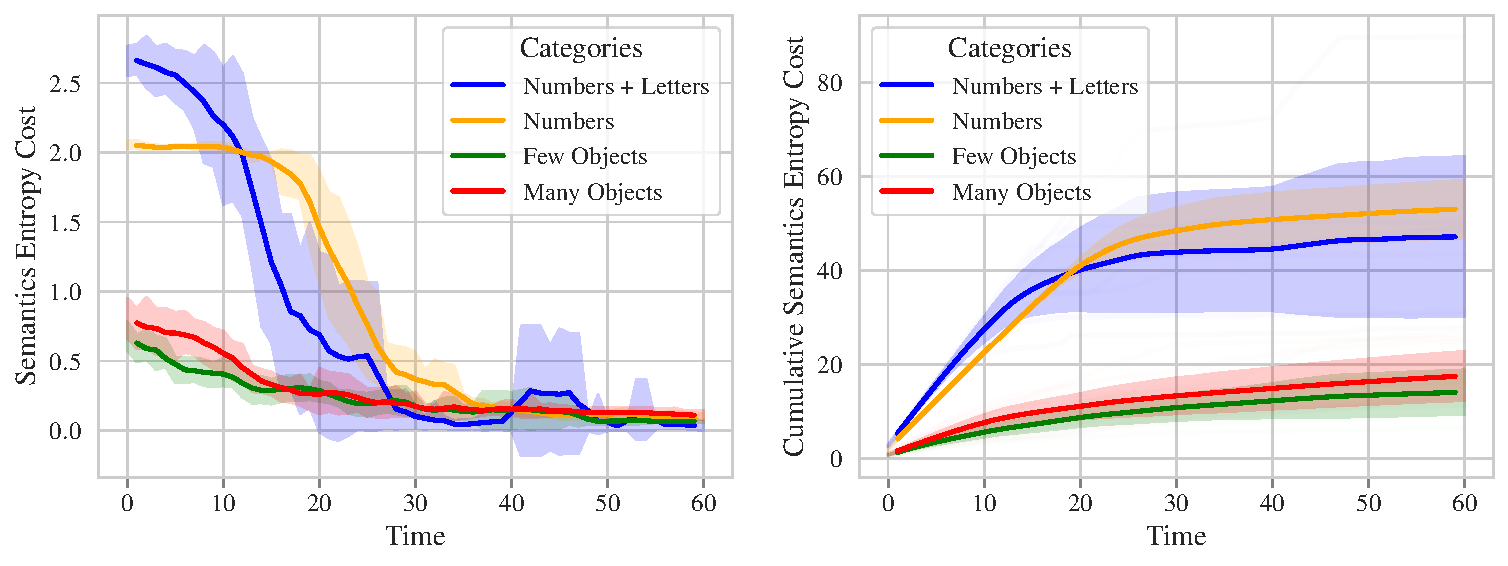
\includegraphics[width=\textwidth]{images/categories_comparison_sgw_rair.pdf}\vspace{6pt}
    % \caption{Effect of categories on semantics entropy reward in ShapeGridWorld. 10 seeds were used.}
    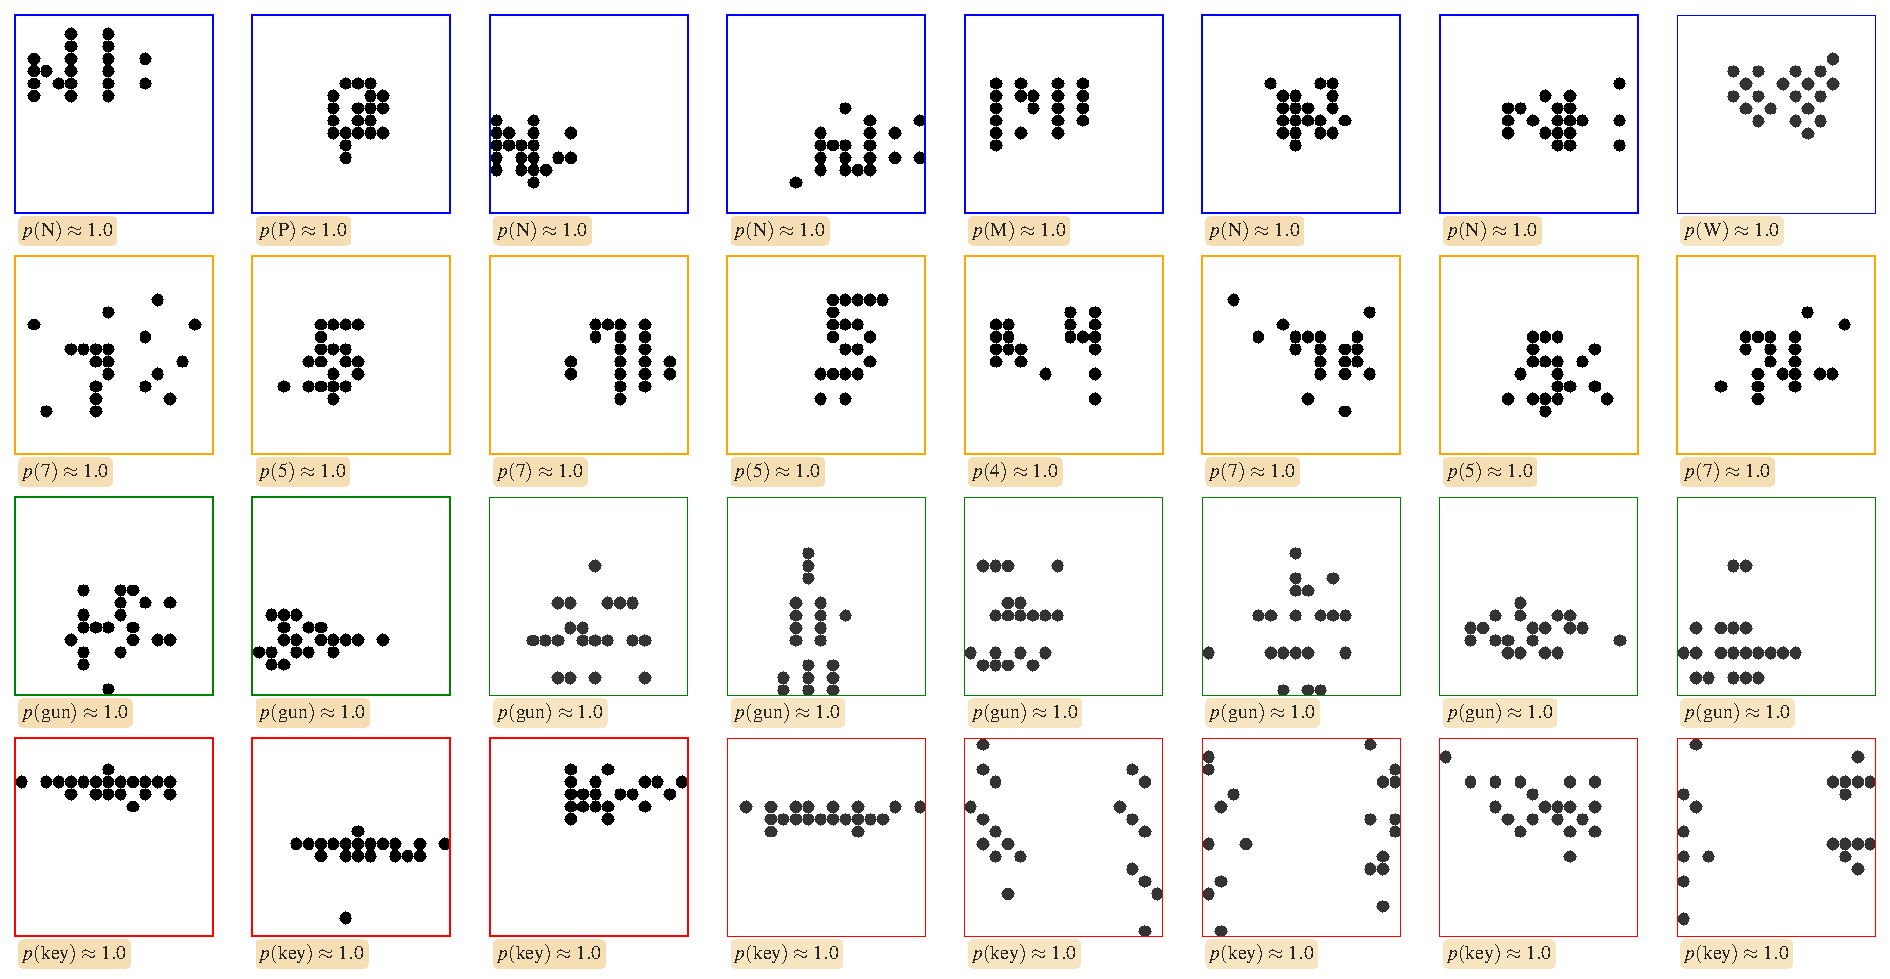
\includegraphics[width=\textwidth]{images/categories_samples_sgw_rair.pdf}\vspace{3pt}
    % \caption{Samples of creations with different categories in ShapeGridWorld.}
    % \label{fig:categories-samples-sgw}
    % \vspace{12pt}
    \captionsetup{justification=centering}
    \caption[Effect of categories on semantics entropy reward in ShapeGridWorld.]{Effect of categories on semantics entropy reward in ShapeGridWorld with RaIR.\\(10 seeds were used.)}
    \label{fig:categories-sgw}
\end{figure}

\begin{figure}[H]
    \centering
    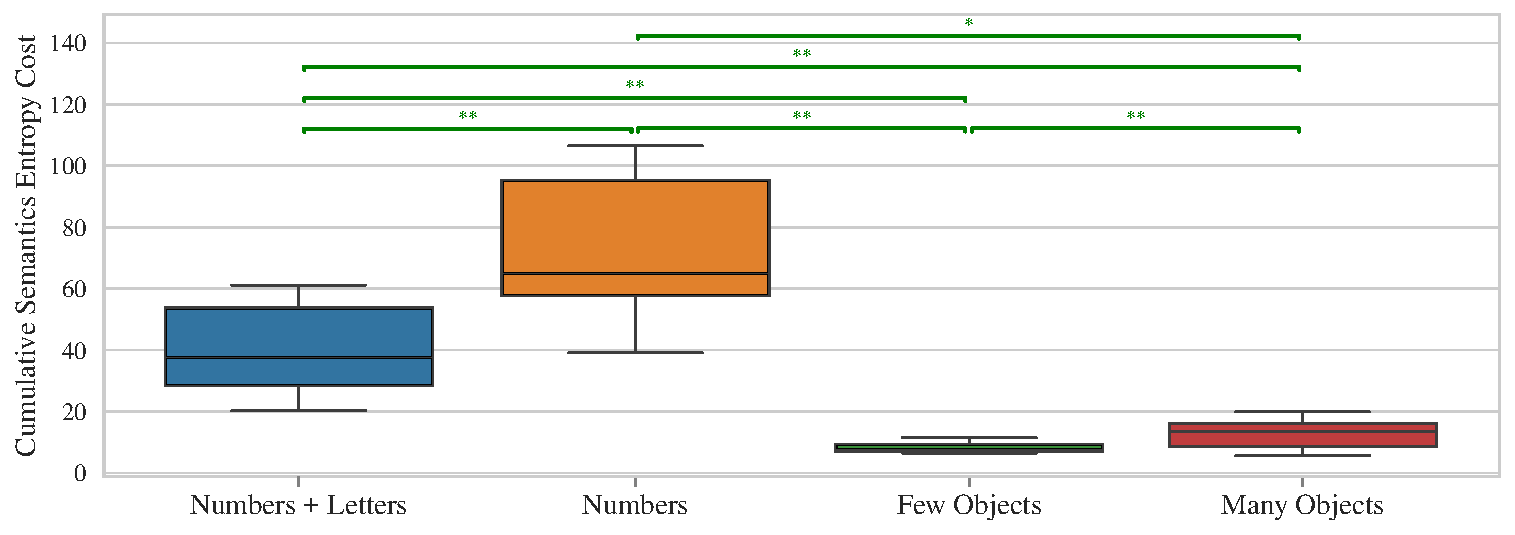
\includegraphics[width=\textwidth]{images/categories_boxplot_sgw_norair_cropped.pdf}\vspace{6pt}
    % \label{fig:categories-boxplot-sgw-norair}
    % \vspace{24pt}
    \includegraphics[width=\textwidth]{images/categories_comparison_sgw_norair_cropped.pdf}\vspace{6pt}
    % \caption{Effect of categories on semantics entropy reward in ShapeGridWorld without RaIR. 10 seeds were used.}
    \includegraphics[width=\textwidth]{images/categories_samples_sgw_norair_cropped.pdf}\vspace{3pt}
    % \caption{Samples of creations with different categories in ShapeGridWorld without RaIR.}
    % \label{fig:categories-samples-sgw-norair}
    % \vspace{12pt}
    \captionsetup{justification=centering}
    \caption[Effect of categories on semantics entropy reward in ShapeGridWorld without RaIR.]{Effect of categories on semantics entropy reward in ShapeGridWorld without RaIR.\\(10 seeds were used.)}
    \label{fig:categories-sgw-norair}
\end{figure}

\begin{figure}[H]
    \centering
    \includegraphics[width=\textwidth]{images/mode_comparison_sgw.pdf}\vspace{6pt}
    \includegraphics[width=0.55\textwidth]{images/mode_samples_sgw.pdf}\vspace{3pt}
    % \caption{Samples of creations with and without grayscale pixels in ShapeGridWorld.}
    % \label{fig:mode-samples-sgw}
    % \vspace{12pt}
    \caption{Effect of the presence of grayscale pixels on semantics entropy reward in ShapeGridWorld.}
    \label{fig:mode-sgw}
\end{figure}

\begin{figure}[H]
    \centering
    \includegraphics[width=\textwidth]{images/n_objects_comparison_sgw.pdf}\vspace{6pt}
    \includegraphics[width=0.55\textwidth]{images/n_objects_samples_sgw.pdf}\vspace{3pt}
    % \caption{Samples of creations with different numbers of objects in ShapeGridWorld.}
    % \label{fig:n-objects-samples-sgw}
    % \vspace{12pt}
    \caption{Effect of the number of objects on semantics entropy reward in ShapeGridWorld.}
    \label{fig:n-objects-sgw}
\end{figure}

\section{Effect of Object Persistency}
\label{sec:sgw-persistency}
% Object Persistency
% object_persistency_comparison_sgw.pdf
% object_persistency_samples_sgw.pdf

We also experimented with the ``object persistency'' of objects in the environment, which defines how many action steps an object is moved before the controller switches its focus on the next object in the predetermined order.
This also included the case of moving all the objects together.
This is related to the step size of the environment which defines how many steps in x/y-directions an object can be moved in one action.

Since the action space with moving all the objects at the same time can be very large (proportional to the number of objects), the controller needs more computational budget to realize the optimal policy, in the form of a higher planning horizon, more sampled trajectories, or more iterations to converge.
We noticed that we obtained the best results when the objects were moved one at a time, only for one timestep, i.e. an object persistency of \(1\), with a step size around a quarter of the grid size.
This is evident from the faster convergence in \figref{fig:object-persistency-sgw}.

\begin{figure}[H]
    \centering
    \includegraphics[width=\textwidth]{images/object_persistency_comparison_sgw.pdf}\vspace{6pt}
    \includegraphics[width=0.55\textwidth]{images/object_persistency_samples_sgw.pdf}\vspace{3pt}
    % \caption{Samples of creations with different object persistency in ShapeGridWorld.}
    % \label{fig:object-persistency-samples-sgw}
    % \vspace{12pt}
    \caption{Effect of object persistency on semantics entropy reward in ShapeGridWorld.}
    \label{fig:object-persistency-sgw}
\end{figure}


\chapter{Additional Graphs}
\label{sec:additional-graphs}

% Class preference in CLIP
\begin{figure}[h]
    \centering
    \includegraphics[width=\textwidth]{images/creations_distribution.pdf}
    \vspace{-12pt}
    \caption[Histogram of creations in our simulations on Tangram showing CLIP's class preference.]{Histogram of creations in our simulations on Tangram showing CLIP's class preference. The choice of classes varied in these simulations; when ``house'' or ``bird'' were present, they were chosen almost all the time. The other creations were obtained only when they were removed. Classes not mentioned in the graph include ``boat'', ``teapot'', ``gun'', ``car'', ``airplane'', ``guitar'', and ``flower''}
    \label{fig:class-preference-tangram}
    \vspace{12pt}
    \includegraphics[width=\textwidth]{images/creations_distribution_sgw.pdf}
    \vspace{-12pt}
    \captionsetup{justification=centering}
    \caption[Histogram of creations in our simulations on SGW showing CLIP's class preference.]{Histogram of creations in our simulations on SGW showing CLIP's class preference.\\The \(36\) classes are all letters and numbers.}
    \label{fig:class-preference-sgw}
\end{figure}

% % alpha_beta-semantics_std_rair.pdf
% \begin{figure}[h]
%     \centering
%     \includegraphics[width=0.96\textwidth]{images/alpha_beta-semantics_std_rair.pdf}
%     \caption{Standard deviation of regularization strength performance on the semantics reward.}
%     \label{fig:alpha_beta-semantics_std_rair}
% \end{figure}

% nobj_mode_rair_sgw_boxplot.pdf
\begin{figure}[h]
    \centering
    \includegraphics[width=\textwidth]{images/nobj_mode_rair_sgw_boxplot.pdf}
    \caption{Effect of the number of objects, grayscale, and RaIR on semantics entropy reward in SGW.}
    \label{fig:nobj-mode-sgw}
\end{figure}

% all inversions of an image
\begin{figure}[h]
    \centering
    \includegraphics[width=0.95\textwidth]{images/tangram_fish_10.pdf}
    \caption[CLIP on different inversions of the same Tangram creation.]{CLIP on different inversions of the same Tangram creation (\(\tau = 0.1\)).}
    \label{fig:clip-tangram-inversions}
\end{figure}


\chapter{Curated Gallery}
\label{sec:gallery}

% curation_bird.pdf
\begin{figure}[H]
    \centering
    \includegraphics[width=\textwidth]{images/curation_bird.pdf}
    \caption{Birds on Tangram.}
    \label{fig:curation_bird}
\end{figure}

% curation_teapot.pdf
% curation_teapot_.pdf
% curation_teapot_all.pdf
\begin{figure}[H]
    \centering
    % \includegraphics[width=\textwidth]{images/curation_teapot.pdf}
    % \includegraphics[width=\textwidth]{images/curation_teapot_.pdf}
    \includegraphics[width=0.5\textwidth]{images/curation_teapot_all.pdf}
    \caption{Teapots on Tangram.}
    \label{fig:curation_teapot}
\end{figure}

% curation_chair.pdf
% curation_chair_cropped.pdf
\begin{figure}[H]
    \centering
    \includegraphics[width=\textwidth]{images/curation_chair_cropped.pdf}
    \caption{Chairs on Tangram.}
    \label{fig:curation_chair}
\end{figure}

% curation_letters.pdf
\begin{figure}[H]
    \centering
    \includegraphics[width=0.824\textwidth]{images/curation_letters.pdf}
    \caption{Letters on Tangram.}
    \label{fig:curation_letters}
\end{figure}

% curation_shirt_all.pdf
\begin{figure}[H]
    \centering
    \includegraphics[width=0.66\textwidth]{images/curation_shirt_all.pdf}
    \caption{Shirts on Tangram.}
    \label{fig:curation_shirt_all}
\end{figure}

% curation_heart.pdf
% curation_heart_all.pdf
\begin{figure}[H]
    \centering
    \includegraphics[width=0.66\textwidth]{images/curation_heart.pdf}
    % \includegraphics[width=0.66\textwidth]{images/curation_heart_all.pdf}
    \caption{Hearts on Tangram.}
    \label{fig:curation_heart}
\end{figure}

% % sgw_reruns.pdf
% \begin{figure}[H]
%     \centering
%     \includegraphics[width=\textwidth]{images/sgw_reruns.pdf}
%     \caption{Letters on ShapeGridWorld.}
%     \label{fig:sgw-trajectories}
% \end{figure}

% curation_animals.pdf
% curation_faces_a.pdf
% curation_faces_all.pdf
\begin{figure}[H]
    \centering
    % \includegraphics[width=\textwidth]{images/curation_animals.pdf}
    % \includegraphics[width=\textwidth]{images/curation_faces_a.pdf}
    \includegraphics[width=0.66\textwidth]{images/curation_faces_all.pdf}
    \captionsetup{margin=72pt}
    \caption[Animals on Tangram.]{Animals on Tangram. It might be difficult to see these creations as animals at first glance.
    Interestingly, this is because they seem to be faces of animals and not outlines as we might expect. We found these faces to have consistent subtle differences that set them apart.}
    \label{fig:curation_animals}
\end{figure}

% curation_house.pdf
\begin{figure}[H]
    \centering
    \includegraphics[width=\textwidth]{images/curation_house.pdf}
    \caption{Houses on Tangram.}
    \label{fig:curation_house}
\end{figure}

% curation_gun_all.pdf
% curation_sgw_objects.pdf
% curation_sgw_objects_cropped.pdf
\begin{figure}[H]
    \centering
    \includegraphics[width=0.5\textwidth]{images/curation_gun_all.pdf}
    \includegraphics[width=0.824\textwidth]{images/curation_sgw_objects_cropped.pdf}
    \caption{Guns on Tangram and ShapeGridWorld.}
    \label{fig:curation_gun_all}
\end{figure}

% % curation_objects.pdf
% \begin{figure}[H]
%     \centering
%     \includegraphics[width=\textwidth]{images/curation_objects.pdf}
%     \caption{Objects on Tangram.}
%     \label{fig:curation_objects}
% \end{figure}

% curation_sgw_letters.pdf
\begin{figure}[H]
    \centering
    \includegraphics[width=\textwidth]{images/curation_sgw_letters.pdf}
    \caption{Letters on ShapeGridWorld.}
    \label{fig:curation_sgw_letters}
\end{figure}

% % curation_sgw_N.pdf
% \begin{figure}[H]
%     \centering
%     \includegraphics[width=\textwidth]{images/curation_sgw_N.pdf}
%     \caption{The letter ``N'' on ShapeGridWorld.}
%     \label{fig:curation_sgw_N}
% \end{figure}

% curation_sgw_numbers.pdf
\begin{figure}[H]
    \centering
    \includegraphics[width=\textwidth]{images/curation_sgw_numbers.pdf}
    \caption{Numbers on ShapeGridWorld.}
    \label{fig:curation_sgw_numbers}
\end{figure}

% % curation_sgw_objects.pdf
% \begin{figure}[H]
%     \centering
%     \includegraphics[width=\textwidth]{images/curation_sgw_objects.pdf}
%     \caption{Objects on ShapeGridWorld.}
%     \label{fig:curation_sgw_objects}
% \end{figure}

% \newpage
% % curation_tree.pdf
% % curation_tree_.pdf
% \begin{figure}[h]
%     \centering
%     \includegraphics[width=\textwidth]{images/curation_tree.pdf}
%     % \includegraphics[width=\textwidth]{images/curation_tree_.pdf}
%     % \caption{Trees on Tangram.}
%     \label{fig:curation_tree}
% \end{figure}

% curation_fish.pdf
% curation_fish_.pdf
% curation_fish_2.pdf
\begin{figure}[H]
    \centering
    \includegraphics[width=\textwidth]{images/curation_fish.pdf}
    % \includegraphics[width=\textwidth]{images/curation_fish_.pdf}
    % \includegraphics[width=\textwidth]{images/curation_fish_2.pdf}
    \caption{Fishes on Tangram.}
    \label{fig:curation_fish}
\end{figure}

\addtocontents{toc}{\protect\setcounter{tocdepth}{2}}

\end{appendices}

\end{document}
